%%%%%%%%%%%%%%%%%%%%%%%%%%%%%%%%%%%%%%%%%
% Tufte-Style Book (Minimal Template)
% LaTeX Template
% Version 1.0 (5/1/13)
%
% This template has been downloaded from:
% http://www.LaTeXTemplates.com
%
% License:
% CC BY-NC-SA 3.0 (http://creativecommons.org/licenses/by-nc-sa/3.0/)
%
% IMPORTANT NOTE:
% In addition to running BibTeX to compile the reference list from the .bib
% file, you will need to run MakeIndex to compile the index at the end of the
% document.
%
%%%%%%%%%%%%%%%%%%%%%%%%%%%%%%%%%%%%%%%%%

%----------------------------------------------------------------------------------------
%	PACKAGES AND OTHER DOCUMENT CONFIGURATIONS
%----------------------------------------------------------------------------------------

\documentclass{tufte-book} % Use the tufte-book class which in turn uses the tufte-common class
%Tufte docs: http://ftp.math.purdue.edu/mirrors/ctan.org/macros/latex/contrib/tufte-latex/sample-book.pdf
\usepackage{geometry}

  \geometry{
    % showframe,
   % paperwidth=8.5in,
    %paperheight=11in,
   % left=0.55in,
   % right=0.45in,
    %top=.5in,
    %bottom=.5in,
    %marginparsep=0.25in,
    %marginparwidth=1in,
   % includemp,
    %includehead,
    % The text width and height are calculated automatically.
  }

\hypersetup{colorlinks,linkcolor=violet} % Comment this line if you don't wish to have colored links
\expandafter\def\expandafter\UrlBreaks\expandafter{\UrlBreaks  \do\-} %  Allow URLs to wrap on dash

\setlength\marginparpush{12pt} %https://tex.stackexchange.com/questions/89098/vertical-spacing-between-sidenotes-and-between-sidenotes-and-captions-in-tuft

\usepackage{pdfpages} % Allow PDF insert for non-TeX elements

\usepackage{microtype} % Improves character and word spacing

\usepackage{lipsum} % Inserts dummy text

\usepackage{booktabs} % Better horizontal rules in tables

\usepackage{graphicx} % Needed to insert images into the document
\graphicspath{{graphics/}} % Sets the default location of pictures
\setkeys{Gin}{width=\linewidth,totalheight=\textheight,keepaspectratio} % Improves figure scaling

\usepackage{upquote}
\usepackage{fancyvrb} % Allows customization of verbatim environments
%Fancyvrb docs: http://mirrors.ibiblio.org/CTAN/macros/latex/contrib/fancyvrb/doc/fancyvrb-doc.pdf
\fvset{fontsize=\small} % The font size of all verbatim text can be changed here

\renewcommand{\FancyVerbFormatLine}{\color{violet}}

\newcommand{\hangp}[1]{\makebox[0pt][r]{(}#1\makebox[0pt][l]{)}} % New command to create parentheses around text in tables which take up no horizontal space - this improves column spacing
\newcommand{\hangstar}{\makebox[0pt][l]{*}} % New command to create asterisks in tables which take up no horizontal space - this improves column spacing

\usepackage{xspace} % Used for printing a trailing space better than using a tilde (~) using the \xspace command

\newcommand{\monthyear}{\ifcase\month\or January\or February\or March\or April\or May\or June\or July\or August\or September\or October\or November\or December\fi\space\number\year} % A command to print the current month and year

\newcommand{\openepigraph}[2]{ % This block sets up a command for printing an epigraph with 2 arguments - the quote and the author
\begin{fullwidth}
\sffamily\large
\begin{doublespace}
\noindent\allcaps{#1}\\ % The quote
\noindent\allcaps{#2} % The author
\end{doublespace}
\end{fullwidth}
}

\newcommand{\blankpage}{\newpage\hbox{}\thispagestyle{empty}\newpage} % Command to insert a blank page

\usepackage{imakeidx} % Used to generate the index
\makeindex % Generate the index which is printed at the end of the document

%So we can use option FloatBarrier, which is similar to [H] but is an
%alternative solition when the algorithm can't solce [H] as too many
%settings are going on. [H] seems to get stuck in infinite loop
%https://tex.stackexchange.com/questions/2275/keeping-tables-figures-close-to-where-they-are-mentioned
\usepackage{placeins}
\newcommand{\codeexample}[2]{
	\begin{figure*}[h]
		\VerbatimInput[
			framesep=3mm,
			frame=lines, % line above and below code section
			numbers=left, %Line number
			label= #1, %name of code section
			baselinestretch=0.75, %Use line space more similat to line space in code editors
		]{#2} %Write the relative file path and the name of the file to be included
	\end{figure*}
	\FloatBarrier
}

%%%%%%%%%%%%%%%%%%%%%%%%%%%%%
% Customizing section/subsection titles
% https://tex.stackexchange.com/questions/96090/formatting-subsections-and-chapters-in-tufte-book

% section format
\titleformat{\section}%
{\normalfont\Large\bfseries}% format applied to label+text
{}% label
{}% horizontal separation between label and title body
{}% before the title body
[]% after the title body

% subsection format
\titleformat{\subsection}%
{\normalfont\itshape\large}% format applied to label+text
{}% label
{}% horizontal separation between label and title body
{}% before the title body
[]% after the title body

%%%%%%%%%%%%%%%%%%%%%%%%%%%
% Making figures full-widths
% https://tex.stackexchange.com/questions/262952/tufte-book-captions-under-figure
 
 \makeatletter
 \renewenvironment{figure}[1][htbp]{%
 	\@tufte@orig@float{figure}[#1]%
 }{%
 	\@tufte@orig@endfloat
 }

%----------------------------------------------------------------------------------------
%	BOOK META-INFORMATION
%----------------------------------------------------------------------------------------

\title{Development \\ \noindent Research \\ \noindent in Practice: \\ \bigskip
\noindent The DIME Analytics \\ \noindent Data Handbook} % Title of the book

\author{Kristoffer Bj{\"a}rkefur \\ \noindent Lu{\'i}za Cardoso de Andrade \\ \noindent Benjamin Daniels \\ \noindent Maria Jones \\} % Author

\publisher{DIME Analytics} % Publisher

%----------------------------------------------------------------------------------------

%--------------------------------------
%	Add URL to commit on copyright page
%--------------------------------------

\usepackage{xstring}
\usepackage{catchfile}

%Set this user input
\newcommand{\gitfolder}{.git} %relative path to .git folder from .tex doc
\newcommand{\reponame}{worldbank/dime-data-handbook} % Name of account and repo be set in URL

%Based on this https://tex.stackexchange.com/questions/455396/how-to-include-the-current-git-commit-id-and-branch-in-my-document
\CatchFileDef{\headfull}{\gitfolder/HEAD}{} 				%Get path to head file for checked out branch
\StrGobbleRight{\headfull}{1}[\head]						%Remove end of line character
\StrBehind[2]{\head}{/}[\branch]							%Parse out the path only
\CatchFileDef{\commit}{\gitfolder/refs/heads/\branch}{}	%Get the content of the branch head
\StrGobbleRight{\commit}{1}[\commithash]					%Remove end of line characted

%Build the URL to this commit based on the information we now have
\newcommand{\commiturl}{\url{https://github.com/\reponame/commit/\commithash}}

%----------------------------------------------------------------------------------------

% Reset the sidenote number each chapter
\let\oldchapter\chapter
\def\chapter{%
  \setcounter{footnote}{0}%
  \oldchapter
}

%----------------------------------------------------------------------------------------


\begin{document}


\includepdf[noautoscale=true, pages=1]{pdf/15633-Analytics_coverFINAL_print.pdf}

\frontmatter

%----------------------------------------------------------------------------------------
%	EPIGRAPH
%----------------------------------------------------------------------------------------

%----------------------------------------------------------------------------------------

\maketitle % Print the title page

%----------------------------------------------------------------------------------------
%	COPYRIGHT PAGE
%----------------------------------------------------------------------------------------

\newpage
\begin{fullwidth}
~\vfill
\thispagestyle{empty}
\setlength{\parindent}{0pt}
\setlength{\parskip}{\baselineskip}
Copyright \copyright\ \the\year\ \\ \thanklessauthor

\bigskip\par\smallcaps{Published by \thanklesspublisher}

\par\smallcaps{\url{https://worldbank.github.com/dime-data-handbook}}

\par Compiled from commit: \newline
\vspace{-0.5cm}
\commiturl

\par Released under a Creative Commons Attribution 4.0 International (CC BY 4.0) license.\newline
\vspace{-0.5cm}
\url{https://creativecommons.org/licenses/by/4.0}

\par\textit{First printing, \monthyear}

\end{fullwidth}

%----------------------------------------------------------------------------------------
%	Edition notes
%----------------------------------------------------------------------------------------

\cleardoublepage
\chapter*{Acknowledgments and notes} % The asterisk leaves out this chapter from the table of contents

\input{auxiliary/notes.tex}

%----------------------------------------------------------------------------------------
%	Abbreviations
%----------------------------------------------------------------------------------------

\cleardoublepage
\chapter*{Abbreviations} % The asterisk leaves out this chapter from the table of contents

\input{auxiliary/abbreviations.tex}

%----------------------------------------------------------------------------------------

\tableofcontents % Print the table of contents

%----------------------------------------------------------------------------------------

% \listoffigures % Print a list of figures

%----------------------------------------------------------------------------------------

% \listoftables % Print a list of tables

%----------------------------------------------------------------------------------------
%	DEDICATION PAGE
%----------------------------------------------------------------------------------------

\cleardoublepage
\thispagestyle{empty}
~\vfill
\begin{doublespace}
\noindent\fontsize{18}{22}\selectfont\itshape
\nohyphenation
Dedicated to all the research assistants who have
wrangled data without being taught how,
hustled to get projects done on time,
wondered if they really should get their PhD after all,
and in doing so made this knowledge necessary and possible.
\end{doublespace}
\vfill
\vfill


%----------------------------------------------------------------------------------------
%	INTRODUCTION
%----------------------------------------------------------------------------------------

\cleardoublepage
\chapter{Introduction: Development Research in Practice}

\begin{fullwidth}
Welcome to \textit{Development Research in Practice: The DIME Analytics Data Handbook}.
This book is intended to teach all users of development data
how to handle data effectively, efficiently, and ethically.
An empirical revolution has changed the face of development research rapidly over the last decade.
Increasingly, researchers are working not just with complex data,
but with \textit{original} data:
datasets collected by the research team themselves
or acquired through a unique agreement with a project partner.
Research teams must carefully document how original data is created, handled, and analyzed.
These tasks now contribute as much weight to the quality of the evidence
as the research design and the statistical approaches do.
At the same time, the scope and scale of empirical research projects is expanding:
more people are working on the same data over longer timeframes.
For that reason, the central premise of this book is that data work is a ``social process''.
This means that the many different people on a team need to have the same ideas
about what is to be done, and when and where and by whom,
so that they can collaborate effectively on a large, long-term research project.

Despite the growing importance of managing data work,
little practical guidance is available for practitioners.
There are few guides to the conventions, standards, and best practices
that are fast becoming a necessity for empirical research.
\textit{Development Research in Practice} aims to fill that gap.
It covers the full data workflow for a complex research project using original data.
We share the lessons, tools, and processes
developed within the World Bank's Development Impact Evaluation (DIME) department,
and compile them into a single narrative of best practices for data work.
This book is not sector-specific;
it will not teach you econometrics,
or how to design an impact evaluation.
There are many excellent existing resources on those topics.
Instead, it will teach you how to think about all aspects of your research from a data perspective,
how to structure research projects to ensure data quality,
and how to institute transparent and reproducible workflows.
We realize that adopting these workflows may have significant upfront learning costs, 
but we are convinced that these investments pay off quickly, 
as you will both save time and improve the quality of your research going forward.


\end{fullwidth}

%------------------------------------------------

\section{How to read this book}
This book aims to be a highly practical resource so the reader can
immediately begin to collaborate more effectively
on large, long-term research projects
that use the methods and tools discussed.
This introduction outlines the basic philosophies
that motivate this book and our approach to research data.
We want all readers to understand at the outset our mindset
that research data work is primarily about
communicating effectively within a team
and that standardization and simplification of data tasks
is a major enabler of effective collaboration.
The main chapters of this book will walk you through the data workflow at each stage
of an empirical research project, from design to publication.
The figure in this introduction visualizes the data workflow.
Chapters 1 and 2 contextualize the workflow,
and set the stage for the hands-on data tasks
which are described in detail in Chapters 3 to 7.

\textbf{Chapter 1} outlines a set of practices and ideals to ensure that
research consumers can be confident in the conclusions reached,
and that the reliability of research work can be verified.
It begins with ethical principles to guide empirical research,
focusing on research reproducibility, transparency, and credibility.
It then introduces tools to document
the aims and methods of a research project,
ensuring that meta-information about your research is available
and that you approach data work with an eye towards the future.

\textbf{Chapter 2} teaches you to structure your data work for collaborative research,
while ensuring the privacy and security of research participants.
It discusses the importance of planning datawork and associated tools in advance,
long before any data is acquired.
It also describes ethical concerns common to development data,
common pitfalls in legal and practical management of data,
and how to respect the rights of research participants at all stages of data work.

\textbf{Chapter 3} turns to the measurement framework,
and how to translate research design to a data work plan.
It details DIME's data map template, a set of tools to communicate the project's data requirements
both across the team and across time.
It also discusses how to implement random sampling and random assignment
in a reproducible and credible manner.

\textbf{Chapter 4} covers data acquisition. It starts with
the legal and institutional frameworks for data ownership and licensing,
to ensure that you are aware of the rights and responsibilities
of using data collected by the research team or by others.
It provides a deep dive on collecting high-quality primary electronic survey data,
including developing and deploying survey instruments.
Finally, it discusses secure data handling during transfer, sharing, and storage,
which is essential in protecting the privacy of respondents in any data.

\textbf{Chapter 5} describes data processing tasks.
It details how to construct ``tidy'' data at the appropriate units of analysis,
how to ensure uniquely identified datasets, and
how to routinely incorporate data quality checks into the workflow.
It also provides guidance on de-identification and cleaning of personally-identified data,
focusing on how to understand and structure data
so that it is ready for indicator construction and analytical work.

\textbf{Chapter 6} discusses data analysis tasks.
It begins with data construction, or the creation of new variables
from the raw data acquired or collected in the field.
It introduces core principles for writing analytical code
and creating, exporting, and storing research outputs
such as figures and tables reproducibly using dynamic documents.

\textbf{Chapter 7} outlines the publication of research outputs,
including manuscripts, code, and data.
This chapter discusses
how to effectively collaborate on technical writing
using dynamic documents.
It also covers how and why to publish datasets
in an accessible, citable, and safe fashion.
Finally, it provides guidelines for preparing
functional and informative reproducibility packages
that contain all the code, data, and meta-information needed
for others to evaluate and reproduce your work.

Each chapter starts with a box which provides a summary of the most important points,
takeaways for different types of readers, 
and a list of key tools and resources for implementing the recommended practices.
After reading each chapter, you should understand
what tasks will be performed at every stage of the workflow,
and how to implement them according to best practices.
You should also understand how the various stages of the workflow tie together,
and what inputs and outputs are required and produced from each.
The references and links contained in each chapter
will lead you to detailed descriptions of individual
ideas, tools, and processes to refer to when you need to implement the tasks yourself.

\subsection*{The DIME Wiki: A complementary resource}
Throughout the book, you will find many references to the DIME Wiki.\sidenote{\url{https://dimewiki.worldbank.org}}
The DIME Wiki is a free online collection of impact evaluation resources and best practices. 
This handbook and the DIME Wiki are meant to go hand-in-hand: 
the handbook provides the narrative structure and workflow, 
and the Wiki dives into specific implementation details,
offers detailed code examples, and 
provides a more exhaustive set of references for each topic. 
Importantly, the DIME Wiki is a living resources that is 
continuously updated and improved,
by the authors of this book and external contributors.
We welcome all readers to register as Wiki users and contribute directly.\sidenote{\url{https://dimewiki.worldbank.org/New_Users}} 

%------------------------------------------------

\begin{fullwidth}
	\begin{figure}
		\centering
		\includegraphics[width=1.5\linewidth]{diagrams/Introduction}
		\caption{Overview of development research data work tasks}
		\label{fig:intro}
	\end{figure}
\end{fullwidth}

%------------------------------------------------

\section{Standardizing data work}

In the past, data work was often treated as a ``black box'' in research.
A published manuscript might exhaustively detail
research designs, estimation strategies, and theoretical frameworks,
but typically reserved very little space for detailed descriptions
of how data was actually collected and handled.
It is almost impossible to assess the quality of the data in such a paper,
and whether the results could be reproduced.
In the past decade, this has started to change,\sidenote{\citet{swanson2020research}}
in part due to increasing requirements by publishers and funders to release code and data.

Data handling and documentation is a key skill for researchers and research staff.
Standard processes and documentation practices
are important throughout the research process to accurately convey
and implement the intended research design,\sidenote{\citet{vilhuber_lars_2020_3911311}}
and to minimizes security risks: 
better protocols and processes lower the probability of data leakages, 
security breaches, and loss of personal information.
When data work is done in an ad-hoc manner,
it is very difficult for others to understand what is being done --
a reader has to simply trust that the researchers did these things right.
Most importantly, if any part of the data pipeline breaks down,
research results become unreliable\sidenote{ \citet{mccullough2008economics}}
and cannot be faithfully interpreted
as being an accurate picture of the intended research design.\sidenote{
  \url{https://blogs.worldbank.org/impactevaluations/more-replication-economics}}
Because we almost never have ``laboratory'' settings\sidenote{
  See \citet{baldwin2015elections} for an example.}
in this type of research,
such a failure has a very high cost:
we will have wasted the investments that were made into knowledge generation,
and the research opportunity itself,
where we intended to conduct the study.\sidenote{\citet{camerer2016evaluating}}

Accurate and reproducible data management and analysis
is essential to the success and credibility of modern research.
Standardizing and documenting data handling processes is essential
to be able to evaluate and understand
the data work alongside any final research outputs.
An important component of this is \textbf{process standardization}.\sidenote{
	\textbf{Process standardization:} Agreement within a research team
	about how all tasks of a specific type will be approached.}\index{process standardization}
Process standardization means that there is
little ambiguity about how something ought to be done,
and therefore the tools to do it can be set in advance.
Standard processes help other people understand your work,
and they also make your work easier to document.
Process standardization and documentation should allow readers of your code to:
(1) quickly understand what a particular process or output is supposed to be doing;
(2) evaluate whether or not it does that thing correctly; and
(3) modify it either to test alternative hypotheses or to adapt into their own work.
This book will discuss specific standards recommended by DIME Analytics,
but we are more interested in convincing the reader
to discuss the adoption of \textit{a} standard within research teams
than to necessarily use \textit{the} particular standards that we recommend.


\section{Standardizing coding practices}

Modern quantitative research relies heavily
on standardized statistical software tools,
written with various coding languages, to standardize analytical work.
Outputs like regression tables and data visualizations
are created using code in statistical software for two primary reasons.
The first is that using a standard command or package ensures that the work is done right,
and the second is that it ensures the same procedure can be confirmed or checked
at a later date or using different data.
Keeping a clear, human-readable record of these code and data structures is critical.
While it is often \textit{possible} to perform nearly all the relevant tasks
through an interactive user interface or even through software such as Excel,
this practice is strongly advised against.
In the context of statistical analysis,
the practice of writing all work using standard code is widely accepted.
To support this practice, DIME now maintains portfolio-wide standards
about how analytical code should be maintained and made accessible
before, during, and after release or publication.

Over the last few years, DIME has extended the same principles to preparing data for analysis,
which often comprises just as much (or more) of the manipulation done to the data
over the life cycle of a research project.
A major aim of this book is to encourage research teams
to think of the tools and processes they use
for designing, collecting, and handling data
just as they do for analytical tasks.
Correspondingly, a major contribution of DIME Analytics
has been tools and standard practices
for implementing these tasks using statistical software.

While we assume that you are going to do nearly all data work using code,
many development researchers come from economics and statistics backgrounds
and often understand code to be a means to an end rather than an output itself.
We believe that this must change somewhat:
in particular, we think that development practitioners
must think about their code and programming workflows
just as methodologically as they think about their research workflows,
and think of code and data as research outputs, just as manuscripts and briefs are.

This approach arises because we see the code as the ``recipe'' for the analysis.
The code tells others exactly what was done,
how they can do it again in the future,
and provides a roadmap and knowledge base for further original work.\sidenote{\citet{hamermesh2007replication}}
Performing every task through written code
creates a record of every task you performed.\sidenote{\citet{ozier2019replication}}
It also prevents direct interaction
with the data files that could lead to non-reproducible processes.\sidenote{\citet{chang2015economics}}
Finally, DIME Analytics has invested a lot of time in developing code as a learning tool:
the examples we have written and the commands we provide
are designed to provide a framework for common practice
across the entire DIME team, so that everyone is able to
read, review, and provide feedback on the work of others
starting from the same basic ideas about how various tasks are done.

Most specific code tools have a learning and adaptation process,
meaning you will become most comfortable with each tool
only by using it in real-world work.
To support your process of learning reproducible tools and workflows,
we reference free and open-source tools wherever possible,
and point to more detailed instructions when relevant.
\textbf{Stata},\sidenote{\citet{statacorp2019stata}}
as a proprietary software, is the notable exception here
due to its persistent popularity in development economics and econometrics.
This book also includes, in an appendix,
the \textbf{DIME Analytics Coding Guide}
which includes instructions for how to write good code,
instructions on how to use the code examples in this book,
as well as our Stata Style Guide.
DIME projects are strongly encouraged to
explicitly adopt and follow coding style guides in their work.
Style guides harmonize code within and across teams
making it easier to understand and reuse code,
which ultimately helps teams to
build on each other's best practices.
Some of the programming languages used at DIME
already have well-established and commonly used style guides,
such as the Tidyverse style guide for R
and PEP-8 for Python.\sidenote{See DIME Analytics Coding Standards:
	\url{https://github.com/worldbank/dime-standards}}.
Stata has relatively few resources of this type available,
which is why we have created and included one here that
we hope will be an asset to all Stata users.

\section{The team behind this book}
DIME is the Development Impact Evaluation department of the World Bank.\sidenote{
	\url{https://www.worldbank.org/en/research/dime}}
Its mission is to generate high-quality and operationally relevant data and research
to transform development policy, help reduce extreme poverty, and secure shared prosperity.\sidenote{\citet{legovini2015impact}}
DIME develops customized data and evidence ecosystems to produce actionable information
and recommend specific policy pathways to maximize impact.
The department conduct research in 60 countries with 200 agencies, leveraging a
US\$180 million research budget to shape the design and implementation of
US\$18 billion in development finance.
DIME also provides advisory services to 30 multilateral and bilateral development agencies.\sidenote{\citet{legovini2019}}
DIME research is organized into four primary topic pillars:
Economic Transformation and Growth;
Gender, Economic Opportunity, and Fragility;
Governance and Institution Building;
and Infrastructure and Climate Change.
Over the years, DIME has employed dozens of research economists,
and hundreds of full-time research assistants, field coordinators, and other staff.
The team has conducted over 325 impact evaluations.
\textit{Development Research in Practice} exists to take advantage of that concentration and scale of research,
to synthesize many resources for data collection and research,
and to make DIME tools available to the larger community of development researchers.

As part of its broader mission, DIME invests in public goods
to improve the quality and reproducibility of development research around the world.
One key early innovation at DIME was the creation of DIME Analytics,
the team responsible for writing and maintaining this book.\sidenote{
	\url{https://www.worldbank.org/en/research/dime/data-and-analytics}}
DIME Analytics is a centralized unit that develops and ensures adoption
of high quality research practices across the department's portfolio.
This is done through an intensive, collaborative innovation cycle:
DIME Analytics onboards and supports research assistants and field coordinators,
provides standard tools and workflows to all teams,
delivers hands-on support when new tasks or challenges arise,
and then develops and integrates lessons from those engagements to bring to the full team.
Resources developed and tested in DIME are converted into public goods
for the global research community, through open-access trainings and open-source tools.
The DIME Analytics Resource Directory appendix provides an introduction to public materials.

DIME Analytics has invested many hours over the past years
learning from data work across DIME's portfolio,
identifying inefficiencies and barriers to success,
developing tools and trainings, and standardizing best-practice workflows adopted in DIME projects.
It has also invested significant energy in the language and materials
used to teach these workflows to new team members,
and, in many cases, in software tools that support these workflows explicitly.
DIME team members often work on diverse portfolios of projects
with a wide range of teammates, and we have found
that standardizing core processes across all projects
results in higher-quality work with fewer opportunities to make mistakes.
In that way, the Analytics team is DIME's method of institutionalizing
tools and practices, developed and refined over time,
that give the department a common base of knowledge and practice.
In 2018, for example, DIME adopted universal reproducibility checks
conducted by the Analytics team;
the lessons from this practice helped move the DIME team
from where 50\% of submitted papers in 2018
required significant revision to pass
to where 64\% of papers passed in 2019 without revision required.


\section{Looking ahead}
While adopting the workflows and mindsets described in this book requires an up-front cost,
it will save you (and your collaborators) a lot of time and hassle very quickly.
In part this is because you will learn how to implement essential practices directly;
in part because you will find tools for the more advanced practices;
and most importantly because you will acquire the mindset of doing research with a high-quality data focus.

For some readers, the amount of new tools and practices recommended in this book may seem daunting.
We know from experience at DIME that full-scale adoption is possible;
in the last few years, the full DIME portfolio has transitioned to 
transparent and reproducible workflows, with a fair share of hiccups along the way.
The authors of this book supported that at-scale transition,
and we hope that by sharing our lessons learned and resources, 
the learning curve for readers will be less steep. 
In the summary boxes at the beginning of each chapter, 
we provide a list of the key tools and resources to help readers prioritize.
We will also offer ``second-best'' practices in many cases, 
suggesting easy-to-implement suggestions to increase transparency and reproducibility,
in cases where full-scale adoption of the recommended workflows is not immediately feasible.
In fact, we encourage teams to adopt one new practice at a time 
rather than rebuild their whole workflow from scratch right away.
We hope that by the end of the book,
all readers will have learned how to handle data more efficiently, effectively and ethically
at all stages of the research process.

\mainmatter


%----------------------------------------------------------------------------------------
%	CHAPTER 1
%----------------------------------------------------------------------------------------


\chapter{Chapter 1: Conducting reproducible, transparent, and credible research}
\label{ch:1}

\input{chapters/1-reproducibility.tex}

%-------------------------------------------------------------------------------
%	CHAPTER 2
%-------------------------------------------------------------------------------

\chapter{Chapter 2: Setting the stage for effective and efficient collaboration}
\label{ch:2}

\input{chapters/2-collaboration.tex}

%-------------------------------------------------------------------------------
%	CHAPTER 3
%-------------------------------------------------------------------------------


\chapter{Chapter 3: Establishing a measurement framework}
\label{ch:3}

\input{chapters/3-measurement.tex}


%-------------------------------------------------------------------------------
%	CHAPTER 4
%-------------------------------------------------------------------------------


\chapter{Chapter 4: Acquiring development data}
\label{ch:4}

%------------------------------------------------

\begin{fullwidth}
Many research questions require the team to acquire original data,
because no source of publicly available data addresses the
inputs or outcomes of interest for the relevant population.
Data acquisition can take many forms, including:
primary data generated through surveys;
private sector partnerships granting access to new data sources, such as administrative and sensor data;
digitization of paper records, including administrative data; web scraping;
primary data capture by unmanned aerial vehicles or other types of remote sensing;
or novel integration of various types of datasets, such as combining survey and sensor data.
Much of the recent push toward credibility in the social sciences has focused on analytical practices.
However, credible development research depends, first and foremost, on the quality of the acquired data.
Clear and careful documentation of the data acquisition process is essential for research reproducibility.

This chapter covers reproducible data acquisition,
special considerations for generating high-quality survey data,
and protocols for safely and securely handling confidential data.
The first section discusses reproducible data acquisition:
how to establish and document your right to use the data.
This applies to all original data,
whether collected for the first time through surveys or sensors or acquired through a unique partnership.
The second section goes into detail on data acquisition through surveys,
as this process is typically more involved than acquisition of secondary data,
and has more in-built opportunities for quality control.
It provides detailed guidance on the electronic survey workflow,
from designing electronic survey instruments to monitoring data quality once fieldwork is ongoing.
The final section discusses safe data handling,
providing guidance on how to receive, transfer, store, and share confidential data.
Secure file management is a basic requirement to comply with the legal and
ethical agreements that allow  access to personal information for research purposes.


\end{fullwidth}

\section{Acquiring data ethically and reproducibly}

Clearly establishing and documenting data access is critical for reproducible research.
This section provides guidelines for
establishing data ownership, receiving data from development partners,
and documenting the research team's right to use the data.
It is the researchers' responsibility to respect the rights
of people who own the data and the people who are described by it;
but also to make sure that information is as available and accessible as possible.
These twin responsibilities can and do come into tension,
so it is important to be fully informed about what other researchers are doing
and to fully inform other researchers of what you are doing.
Writing down and agreeing to specific details is a good way of doing that.


\subsection{Determining data ownership}
Before acquiring any data, it is critical to establish data ownership.
Data ownership\sidenote{More details and best practices related to data ownership
	can be found on the DIME Wiki: \url{https://dimewiki.worldbank.org/Data\_Ownership}}\index{data ownership}
can sometimes be challenging to establish,
as various jurisdictions have differing laws regarding data and information,
and the research team may have their own information regulations.\sidenote{
	More details and best practices related to data ownership
	can be found on the DIME Wiki:
	\url{https://dimewiki.worldbank.org/Data_Ownership}}
In some, data is implicitly owned by the people who it is about.
In others, it is owned by the people who collected it.
In still more, it is highly unclear and there are varying norms.
The best approach is always to consult with a local partner,
and enter into specific legal agreements establishing ownership,
access, and publication rights.
This is particularly critical where confidential data is involved
-- that is, when people are disclosing information to you
that you could not obtain simply by observation or through public records.

If the research team is requesting access to existing data,
they must enter into data licensing agreements\index{data licensing}
to access the data and publish research outputs based on it.
These agreements should make clear from the outset whether and how the
research team can make the original data public, or publish any portion or derivative of the data.\sidenote{
	\textbf{Derivatives} of data can be indicators, aggregates,
	visualizations, etc. created from the original data.}
If the data is publicly accessible,
this may be as simple to agreeing to terms of use on the website where the data can be downloaded.
If it is original data that is not yet publicly accessible,
the process is typically more complex and requires a documented legal agreement or memorandum of understanding.

If the research team is generating data directly, such as survey data,
it is important to clarify up front who owns the data,
and who will have access to it.
These details need to be shared with respondents when they are offered the opportunity
to consent to participate in the study.
If the research team is not collecting the data directly --
for example, if a government, private company, or research partner is doing the data collection --
make sure that you have an explicit agreement
about who owns the resulting data.

The contract for data collection should include specific terms
as to the rights and responsibilities of each stakeholder.
It must clearly stipulate which party owns the data produced,
and that the research team maintains full intellectual property rights.
The contract should also explicitly indicate that the contracted firm
is responsible for protecting respondent privacy,
that the data collection will not be delegated to any third parties,
and that the data will not be used by the firm or subcontractors for any purpose not expressly stated in the contract,
before, during or after the assignment.
The contract should also stipulate that the vendor is required to comply with
ethical standards for social science research,
and adhere to the specific terms of agreement with the relevant
Institutional Review Board (IRB)\sidenote{
	More details and best practices for how to
	submit a project for an IRB approval
	can be found on the DIME Wiki:
	\url{https://dimewiki.worldbank.org/IRB\_Approval}}
or applicable local authority.
Finally, it should include policies on reuse, storage, and retention or destruction of data.

Research teams that acquire original data must also consider data ownership downstream,
through the terms they will use to release that data to other researchers or to the general public.
The team should consider whether they can publish the data in full after removing personal identifiers.
For example, the team must consider whether it would be acceptable for
their data to be copied and stored on servers anywhere in the world,
whether they would prefer to manage permissions on a case-by-case basis,
and whether they expect that data users would cite or credit them.
Similarly, the team can require users in turn to release
their derivative datasets or publications under similar licenses,
or offer use without restriction.
There are simple license templates for offering many of these permissions,
but, at the planning stage, the team should make sure
that all licensing agreements, data collection contracts,
and informed consent processes
used to acquire the data specifically detail those future uses.


\subsection{Obtaining data licenses}

Data licensing\sidenote{More details on data licensing agreements can be found on the DIME Wiki:
	\url{https://dimewiki.worldbank.org/Data_License_Agreement}}
is the formal act of the dataset owner
giving some data rights to a specific user,
while retaining ownership of the dataset.
If you are not the owner of the dataset you want to analyze,
you must enter into a licensing agreement to access it for research purposes.
Similarly, when you own a dataset,
you must consider whether you will make the dataset accessible to other researchers,
and what terms-of-use you require.

If the research team requires access to existing data for novel research,
terms of use should be agreed on with the data owner,
typically through a data licensing agreement.
These terms should specify what data elements will be received,
what purposes the data will be used for, and who will have access to the data.
Keep in mind that the data owner is likely not highly familiar
with the research process, and therefore may be surprised
at some of the things you want to do if you are not clear up front.
You will typically want intellectual property rights to all research outputs developed used the data,
a license for all uses of derivative works, including public distribution
(unless ethical considerations contraindicate this).
This is important to allow the research team to store, catalog, and publish, in whole or in part,
either the original licensed dataset or datasets derived from the original.
Make sure that the license you obtain from the data owner allows these uses,
and that you consult with the owner
if you foresee exceptions with specific portions of the data.

The World Bank has a template Data License Agreement which DIME follows.
The template specifies the specific objectives of the data sharing,
and whether the data can be used only for the established purpose
or for other objectives after it is obtained.
It classifies the data into one of four access categories,
depending on who can access the data by default
and whether case-by-case authorization for access is needed.
The data provider may impose similar restrictions
to sharing derivative data and any or all of the associated metadata.
The template also specifies the required citation for the data.
While you do not need to use the World Bank's template
or its access categories if you do not work on a World Bank project,
we still think it is important that you use this information in two ways.
First, make sure to base your Data License Agreement on some template.
Hand-written agreements can leave many legal ambiguities or gaps
where the permissions given to the research team are unclear or incomplete.
Second, we strongly recommend you to categorize data using some variation of this system.
Then you should have different standard procedures for each category,
so that the intended processes for handling the data are clear.


\subsection{Documenting data received from partners}

Research teams granted access to existing data may receive that data in a number of different ways.
You may receive access to an existing server,
physical access to extract certain information,
or a one-time data transfer.
In all cases, you must take action to ensure
that data is transferred through
secure channels so that confidentiality is not compromised.
See the section \textit{Handling data securely} later in this chapter for how to do that.
Keep in mind that compliance with ethical research standards may
in some cases require a stricter level of security than initially proposed by the partner agency.
It is also critical at this stage to request any and all available documentation for the data;
this could take the form of a data dictionary or codebook,
a manual for administrative data collection system, detailed reports or operating procedures,
or another format.
If no written documentation is available,
interview the person(s) responsible for managing the data
to learn as much as possible about the data;
the interview notes should be archived with data documentation.

At this stage, it is very important to assess
documentation and cataloging of the data and associated metadata.
It is not always clear what pieces of information will jointly constitute a research dataset,
and many of the datasets you receive will not be organized for research.
You should always retain the original data exactly as received
alongside a copy of the corresponding ownership agreement or license.
You should make a simple \texttt{README} document noting the date of receipt,\index{README}
the source and recipient of the data,
and a brief description of each file received.
All too often data will be provided as vaguely-named spreadsheets,
or digital files with non-specific titles,
and documentation will be critical for future access and reproducibility.

Eventually, you will want to make sure that you are creating a set of documents
that can be properly submitted to a data catalog and given a reference and citation.
The metadata -- documentation about the data -- is critical for future use of the data.
Metadata should include documentation of how the data was created,
what they measure, and how they are to be used.
In the case of survey data, this includes the survey instrument and associated manuals;
the sampling protocols and field adherence to those protocols, and any sampling weights;
what variable(s) uniquely identify the dataset(s), and how different datasets can be linked;
and a description of field procedures and quality controls.
DIME uses as a standard the Data Documentation Initiative (DDI), which is supported by the
World Bank's Microdata Catalog.\sidenote{\url{https://microdata.worldbank.org}}

As soon as the desired pieces of information are stored together,
think about which ones are the components of what you would call a dataset.
Often, when you are receiving data from a partner,
even highly-structured materials such as registers or records
are not, as received, equivalent to a research dataset,
and require initial cleaning, restructuring, or recombination
to reach the stage we would consider a raw research dataset.
This is as much an art than a science:
you want to keep information together that is best contextualized together,
but you also want to information granular as much as possible,
particularly when there are varying units of observation.
There usually won't be a single correct way to answer this question,
and the research team will need to decide how to organize the materials received.
Soon, you will begin to build research datasets from this set of information,
and these will become your original clean data,
which will be the material published, released, and cited
as the starting point of your data.
(If funders or publishers request that ``raw'' data be published or cataloged,
for example, this is the dataset that you should provide,
unless they specifically require data in the original format you received it.)
These first datasets created from the received materials
are the objects you need to catalog, release, and license.
Now is a good time to begin assessing disclosure risk
and/or seek publication licenses in collaboration with data providers,
while you are in close contact with them.



%------------------------------------------------


\section{Collecting high-quality data using electronic surveys}
In this section, we detail specific considerations
for acquiring high-quality data through electronic surveys of study subjects.
If your project will not use any survey data, you may want to skip this section.
There are many excellent resources on questionnaire design and field supervision,
but few that cover the particular challenges and opportunities presented by electronic surveys.
There are also many survey software options available to researchers,
and the market is rapidly evolving.
Therefore, we focus on specific workflow considerations for digitally-collected data,
and on basic concepts rather than software-specific tools.

Electronic data collection technologies
have greatly accelerated our ability to bring in high-quality data
using purpose-built survey instruments,
and therefore improved the precision of research.
At the same time, electronic surveys create new pitfalls to avoid.
Programming electronic surveys efficiently requires a very different mindset
than writing paper-based surveys;
careful preparation can improve survey efficiency and data quality.
This section will outline the major steps and technical considerations
you will need to follow whenever you field a custom survey instrument,
no matter the scale.

\subsection{Designing survey instruments}
A well-designed questionnaire results from careful planning,
consideration of analysis and indicators,
close review of existing questionnaires,
survey pilots, and research team and stakeholder review.
There are many excellent resources on questionnaire design,
such as from the World Bank's Living Standards Measurement Survey.\sidenote{\citet{glewwe2000designing}}
The focus of this section is the design of electronic field surveys,
often referred to as Computer Assisted Personal Interviews (CAPI).\sidenote{
	More details and links to CAPI resources can be found on the DIME Wiki:
  \url{https://dimewiki.worldbank.org/Computer-Assisted\_Personal\_Interviews\_(CAPI)}}
Although most surveys are now collected electronically, by tablet, mobile phone or web browser,
\textbf{questionnaire design}\sidenote{
  More details and links to questionnaire design resources
	can be found on the DIME Wiki:
  \url{https://dimewiki.worldbank.org/Questionnaire\_Design}}
  \index{questionnaire design}
(content development) and \textbf{questionnaire programming}\sidenote{
	More details and links to questionnaire programming resources
	can be found on the DIME Wiki:
  \url{https://dimewiki.worldbank.org/Questionnaire\_Programming}}
(functionality development) should be seen as two strictly separate tasks.
Therefore, the research team should agree on all questionnaire content
and design a version of the survey on paper
before beginning to program the electronic version.
This facilitates a focus on content during the design process
and ensures teams have a readable, printable version of their questionnaire.
Most importantly, it means the research, not the technology,
drives the questionnaire design.

We recommend this approach for three reasons.
First, an easy-to-read paper questionnaire
is very useful for training data collection staff,
which we will discuss further in the enumerator training section below.
Second, finalizing the paper version of the questionnaire before beginning any programming
avoids version control concerns that arise from concurrent work
on paper and electronic survey instruments.
Third, a readable paper questionnaire is a necessary component of data documentation,
since it is difficult to work backwards from the survey program to the intended concepts.

The workflow for designing a questionnaire will feel much like writing an essay:
begin from broad concepts and slowly flesh out the specifics.\sidenote{More details
	and links to questionnaire design resources can be found on the DIME Wiki:
  \url{https://dimewiki.worldbank.org/Questionnaire_Design}}\index{questionnaire design}
It is essential to start with a clear understanding of the
\textbf{theory of change}\sidenote{
  More details and links to more resources about theories of change
	can be found at the DIME Wiki:
  \url{https://dimewiki.worldbank.org/Theory\_of\_Change}}\index{theory of change}
and \textbf{research design}\sidenote{
  More details on causal research designs can be found on the DIME Wiki:
  \url{https://dimewiki.worldbank.org/Experimental_Methods}
	and \url{https://dimewiki.worldbank.org/Quasi-Experimental_Methods}}\index{research design}
  for your project.
The first step of questionnaire design is to list key outcomes of interest,
as well as the main covariates to control for and any variables needed for the specific research design.
The ideal starting point for this is a \textbf{pre-analysis plan}.\sidenote{
	More details on how to prepare a pre-analysis plans
	and links to additional resources
	can be found on the DIME Wiki:
  \url{https://dimewiki.worldbank.org/Pre-Analysis\_Plan}}\index{pre-analysis plan}

Use the list of key outcomes to create an outline of questionnaire \textit{modules}.
Do not number the modules; instead use a short prefix
as numbers quickly get outdated when modules are reordered.
For each module, determine if the module is applicable to the full sample,
or only to specific respondents,
and whether or how often the module should be repeated.
A few examples:
a module on maternal health only applies
to households with a woman who has children,
a household income module should be answered
by the person responsible for household finances,
and a module on agricultural production
might be repeated for each crop the household cultivated.
Each module should then be expanded
into specific indicators to observe in the field.\sidenote{
  Links to resources with extensive survey libraries with
	modules that can be used as starting points can be found on the DIME Wiki:
  \url{https://dimewiki.worldbank.org/Literature\_Review\_for\_Questionnaire}}
Questionnaires for impact evaluation
must also include ways to document the reasons for \textbf{attrition} and
treatment \textbf{contamination}.\index{attrition}\index{contamination}
These are essential data components for completing CONSORT records,
a standardized system for reporting enrollment, intervention allocation, follow-up,
and data analysis through the phases of a randomized trial.\sidenote{\citet{begg1996improving}}

\subsection{Piloting survey instruments}
A \textbf{survey pilot} is critical to finalize survey design.\sidenote{More details on
	how to plan, prepare for, and implement a comprehensive survey pilot,
	and links to complementary resources can be found on the DIME Wiki:
	\url{https://dimewiki.worldbank.org/Survey\_Pilot}}\index{survey pilot}
The pilot must be done out-of-sample,
but in a context as similar as possible to the study sample.\sidenote{
	More details on selecting appropriate respondents for a survey pilot
	can be found on the DIME Wiki:
	\url{https://dimewiki.worldbank.org/Survey\_Pilot\_Participants}}
The survey pilot includes three steps:
a \textbf{pre-pilot}, a \textbf{content-focused pilot}, and a \textbf{data-focused pilot}.\sidenote{
	A checklist for how to prepare for a survey pilot can be found on the DIME Wiki:
	\url{https://dimewiki.worldbank.org/Checklist:_Preparing_for_a_Survey_Pilot.}}

The first step is a \textbf{pre-pilot}.
The pre-pilot is a qualitative exercise, done early in the questionnaire design process.
The objective is to answer broad questions about how to measure key outcome variables,
and gather qualitative information relevant to any of the planned survey modules.
A pre-pilot is particularly important when designing new survey instruments.

The second step is a \textbf{content-focused pilot}.
The objectives at this stage are to improve the structure and length of the questionnaire,
refine the phrasing and translation of specific questions,
check for potential sensitivities and for enumerator/respondent interactions,
and confirm coded response options are exhaustive.\sidenote{
  A checklist for content-focused pilots can be found on the DIME Wiki:
	\url{https://dimewiki.worldbank.org/Checklist:\_Content-focused\_Pilot}}
In addition, it is an opportunity to test and refine all survey protocols,
such as how units will be sampled or pre-selected units identified.\sidenote{
	A checklist for survey protocols that should be tested during a survey pilot
	can be found on the DIME Wiki:
	\url{https://dimewiki.worldbank.org/Checklist:\_Piloting\_Survey\_Protocols}}
The content-focused pilot is best done on pen and paper, before the questionnaire is programmed,
because changes at this point may be deep and structural,
which are hard to adjust in code.
It is important at this point to test both the validity and the reliability
of the survey questions;
for this reason it is important to conduct the content-focused pilot
with a sufficiently large sample (the exact requirement will depend on the research sample;
a very rough rule of thumb is a minimum of 30 interviews.

The final stage is a \textbf{data-focused pilot}.
After the content is finalized, proceed with programming a draft version
of the electronic survey instrument.
The objective of this pilot is to refine the questionnaire programming;
this is discussed in detail in the following section.


\subsection{Programming electronic survey instruments}
Once the team is satisfied with the content and structure of the survey,
it is time to move on to implementing it electronically.
Electronic data collection has great potential
to simplify survey implementation and improve data quality.
But it is critical to ensure that electronic survey instruments
flow correctly and produce data that can be used in statistical software,
before data collection starts.
Electronic questionnaires are typically developed
in a spreadsheet (usually using Excel or Google Sheets)
or a software-specific form builder,
all of which are accessible even to novice users.
We will not address software-specific form design in this book;
rather, we focus on coding and design conventions that are important to follow
for electronic surveys regardless of software choice.\sidenote{
  At the time of publishing this book,
	SurveyCTO was the most commonly used survey software at DIME.
	Best practices for SurveyCTO code
	(that almost always applies to other survey software as well)
	can be found on the DIME Wiki:
  \url{https://dimewiki.worldbank.org/SurveyCTO\_Coding\_Practices}}
Survey software tools provide a wide range of features
designed to make implementing even highly complex surveys
easy, scalable, and secure.
However, these are not fully automatic:
you need to actively design and manage the survey.
Here, we discuss specific practices that you need to follow
to take advantage of electronic survey features
and ensure that the exported data
is compatible with your statistical software.

From a data perspective, questions with \textbf{coded response options}\sidenote{
  \textbf{Coded response options:} Responses to questions which require respondents
  to select from a list of choices, corresponding to underlying numerical response codes.}\index{coded response options}
are always preferable to \textbf{open-ended questions}.\sidenote{
  \textbf{Open-ended questions:} Responses to questions which do not
  impose any structure on the response, typically recorded as free-flowing text.}\index{open-ended questions}
The content-based pilot is an excellent time to ask open-ended questions
and refine fixed responses for the final version of the questionnaire --
do not count on coding up lots of free text after a full survey.
Coding responses helps to ensure that the data
will be useful for quantitative analysis.
Two examples help illustrate the point.
First, instead of asking ``How do you feel about the proposed policy change?'',
use techniques like \textbf{Likert scales}.\sidenote{
  \textbf{Likert scale:} an ordered selection of choices indicating the respondent's level of agreement or disagreement with a proposed statement.}
Second, if collecting data on things like medication use or food supplies, you could collect:
the brand name of the product; the generic name of the product; a coded identifier for the item;
or the broad category to which each product belongs
(``antibiotics'' or ``staple foods'', for example).\sidenote{
  See \citet{wafula2017examining} for an example.}
All four may be useful for different reasons,
but the latter two are likely to be the most useful for rapid data analysis.
The coded identifiers require providing a translation dictionary to field staff,
but enables automated rapid recoding for analysis with no loss of information.
The broad category requires agreement on the groups of interest,
but allows for much more comprehensible top-line statistics and data quality checks.
Rigorous field testing is required to ensure that answer categories are comprehensive;
however, it is best practice to include an \textit{other, specify} option.
Keep track of those responses in the first few weeks of field work.
Adding an answer category for a response frequently showing up as \textit{other} can save time,
as it avoids extensive post-coding.

It is essential to name the fields in your questionnaire
in a way that will also work in your data analysis software.
Most survey programs will not enforce this by default,
since limits vary across statistical software,
and survey software will encourage you
to use long sentences as question labels
and detailed descriptions as choice options.
This is what you want for the enumerator-respondent interaction,
but you should already have analysis-compatible labels programmed in the background
so the resulting data can be rapidly imported in analytical software.
There is some debate over how exactly individual questions should be identified:
formats like \texttt{hq\_1} are hard to remember and unpleasant to reorder,
but formats like \texttt{hq\_asked\_about\_loans} quickly become cumbersome.
We recommend using descriptive names with clear prefixes so that variables
within a module stay together when sorted alphabetically.\sidenote{
  More details on naming conventions can be found on the DIME Wiki:
  \url{https://dimewiki.worldbank.org/Naming_Conventions\#Variable_Names}}\index{variable naming}
Variable names should never include spaces or mixed cases
(we prefer all-lowercase naming).
Take special care with the length: very long names will be cut off in some softwares,
which could result in a loss of uniqueness and lots of manual work to restore compatibility.
We further discourage explicit question numbering,
at least at first, as it discourages re-ordering questions,
which is a common recommended change after the pilot.
In the case of follow-up surveys, numbering can quickly become convoluted,
too often resulting in uninformative variables names like
\texttt{ag\_15a}, \texttt{ag\_15\_new}, \texttt{ag\_15\_fup2}, and so on.

\subsection{Using electronic survey features to enhance data quality}
Electronic surveys are more than simply
a paper questionnaire displayed on a mobile device or web browser.
All common survey software allows you to automate survey logic
and include hard or soft constraints on survey responses.
These features make enumerators' work easier,
and they create the opportunity to identify and resolve
data issues in real time,
simplifying data cleaning and improving response quality.
Well-programmed questionnaires should include
most or all of the following features:

\begin{itemize}
  \item{\textbf{Localization}}: the survey instrument should display full-text questions and responses in all potential survey languages, and it should also have English and code-compatible versions of all text and labels.
	\item{\textbf{Survey logic}}: built-in tests should be included for all logic connections between questions, so that only relevant questions appear, rather than relying on enumerators to follow complex survey logic. This covers simple skip codes, as well as more complex interdependencies (e.g., a child health module is only asked to households that report the presence of a child under 5).
	\item{\textbf{Range checks}}: add range checks for all numeric variables to catch data entry mistakes (e.g. \texttt{age} must be less than 120).
	\item{\textbf{Confirmation of key variables}}: require double entry of essential information (such as a contact phone number in a survey with planned phone follow-ups), with automatic validation that the two entries match and rejection and re-entry otherwise.
	\item{\textbf{Multimedia}}: electronic questionnaires facilitate collection of images, video, and geolocation data directly during the survey, using the camera and GPS built into the tablet or phone.
	\item{\textbf{Preloaded data}}: data from previous rounds or related surveys can be used to prepopulate certain sections of the questionnaire, and validated during the survey.
	\item{\textbf{Filtered response options}}: filters reduce the number of response options dynamically (e.g. filtering a ``cities'' choice list based on the state selected).
	\item{\textbf{Location checks}}: enumerators submit their actual location using in-built GPS, to confirm they are in the right place for the interview.
	\item{\textbf{Consistency checks}}: check that answers to related questions align, and trigger a warning if not so that enumerators can probe further (e.g., if a household reports producing 800 kg of maize, but selling 900 kg of maize from their own production).
	\item{\textbf{Calculations}}: make the electronic survey instrument do all math, rather than relying on the enumerator or asking them to carry a calculator.
\end{itemize}

All established survey software include debugging and test options
to correct syntax errors and make sure that
the survey instruments will successfully compile.
This is not sufficient, however, to ensure that the resulting dataset
will load without errors in your data analysis software of choice.
DIME Analytics developed the \texttt{ietestform} command,\sidenote{
	Read more about how to install and use \texttt{ietestform}
	and the reasoning for all the tests it performs on the DIME Wiki:
  \url{https://dimewiki.worldbank.org/ietestform}}\index{ietestform}
part of the Stata package \texttt{iefieldkit}\index{iefieldkit},\sidenote{
  \citet{bjarkefur2020iefieldkit}}
to implement a form-checking routine for \textbf{SurveyCTO},
a proprietary implementation of the open source \textbf{Open Data Kit (ODK)} software.
Intended for use during questionnaire programming and before field work,
\texttt{ietestform} tests for best practices
in coding, naming and labeling, and choice lists.
Although \texttt{ietestform} is software-specific,
many of the tests it runs are general and important to consider regardless of software choice.
To give a few examples, \texttt{ietestform} tests that no variable names exceed
32 characters, the limit in Stata (variable names that exceed that limit will
be truncated, and as a result may no longer be unique).
It checks whether ranges are included for numeric variables.
\texttt{ietestform} also removes all leading and trailing blanks from response lists,
which could be handled inconsistently across software.

The final stage of survey piloting, the data-focused pilot, should be done at this stage (after the questionnaire is programmed).
The objective of this \textbf{data-focused pilot}\sidenote{
  A checklist with best practices important to remember during a data-focused pilot
	can be found on the DIME Wiki:
  \url{https://dimewiki.worldbank.org/Checklist:_Data-focused_Pilot}}
is to validate the programming and export a sample dataset.
Significant desk-testing of the instrument is required to debug the programming
as fully as possible before going to the field.
It is important to plan for multiple days of piloting,
so that any debugging or other revisions to the electronic survey instrument
can be made at the end of each day and tested the following, until no further field errors arise.
The data-focused pilot should be done in advance of enumerator training.

\subsection{Training enumerators}
Once a survey instrument is designed, piloted on paper to refine content,
programmed, piloted electronically to refine the data,
and fully translated to any local languages,
it is time to prepare to train the field staff who will be
responsible for conducting interviews.
The following guidelines for enumerator training apply regardless of
whether data will ultimately be collected in person or remotely,
with the only significant differences being in terms of survey protocols and
the nature of the field practice (which could be in-person or by phone).

The first step is to develop a detailed \textbf{enumerator manual}.\sidenote{
  For more details on how to design an enumerator manual
  and a template for enumerator manuals
  see the DIME Wiki:
  \url{https://dimewiki.worldbank.org/Enumerator\_Training\#Enumerator\_manual}}
	\index{enumerator manual}
The manual should explain each question in the survey instrument,
address any issues that arose during piloting
and cover frequently asked questions.
The manual must also describe survey protocols and conventions,
such as how to select or confirm the identity of respondents,
and standardized means for recording responses such as ``Don't know''.\sidenote{
  For more details and examples of common survey protocols
  see the DIME Wiki:
  \url{https://dimewiki.worldbank.org/Survey\_Protocols}}
\index{survey protocols}
The enumerator manual serves as the basis for the \textbf{enumerator training}.
	\index{enumerator training}
We recommend the training to be divided into two sessions:
first a training-of-trainers, and then the enumerator training.
The training-of-trainers should include the field supervisors
and any other relevant management staff from the organization responsible for data collection,
and should be led by the research team.
The objective is to ensure the survey leaders are
deeply familiar with the survey instrument and protocols,
so that they can support and supervise enumerators going forward.
The training-of-trainers typically lasts a few days,
though exact length will depend on the complexity of the
survey instrument and experience level of the staff.

Enumerator training includes all field staff,
and should be jointly led by the research team
and the survey managers.\sidenote{
  More deatails and best practices related to enumerator trainings
  can be found on the DIME Wiki:
  \url{https://dimewiki.worldbank.org/Enumerator\_Training}}
This training typically lasts one to two weeks,
though exact length will depend on complexity and experience;
training for particularly challenging surveys may take a full month.
Enumerator training has three components: review of the paper questionnaire,
review of the electronic survey instrument, and field practice.
The training schedule should allow for significant discussion and feedback
after each component.
Training with a paper survey instrument is critical,
even for surveys that will be deployed electronically.
Starting with paper ensures a focus on survey content and structure
before diving into the technical components of the survey software.
It is much easier for enumerators to understand
the overall flow of a survey instrument and
the range of possible participant responses
on a paper survey than on a tablet,
and it is easier to translate that understanding to
digital functionality later.\sidenote{
  DIME Analytics developed standard guidelines
  for introducing field staff to the survey software DIME
  uses most commonly, SurveyCTO:
  \url{https://osf.io/n7ctd/}}
The classroom training should be very interactive, using methods such as role plays
and mock interviews to test understanding of survey protocols and modules.
The field practice should be carefully supervised,
so as to provide individualized feedback to each enumerator.

When introducing the digital form of the survey,
enumerators should submit data from practice interviews to the server,
and the research team should run the standard data quality checks,
to familiarize the enumerators with those standards for data quality
and how quality issues will be communicated and resolved.
It is essential to train more enumerators than will be required
for the survey,
and to include objective assessments throughout the training.\sidenote{
  More details on enumerator assessment metrics
  can be found on the DIME Wiki:
  \url{https://dimewiki.worldbank.org/Enumerator\_Training\#Assessing\_Enumerators}}
These assessments can take the form of pop quizzes (which we recommend doing daily,
using the same software as the survey), points for participation,
and score on the field practice.
At the end of the training, use the aggregate score to transparently select the final team of enumerators.


\subsection{Checking data quality in real time}
Once all field staff are trained, it is time to start collecting data.
If you have followed all the guidance above, the stage should be set for quality data.
To ensure high quality data in practice,
the research team should develop a \textbf{data quality assurance plan}.\sidenote{
  More details on how to develop a data quality assurance plan
  can be found on the DIME Wiki:
  \url{https://dimewiki.worldbank.org/Data\_Quality\_Assurance\_Plan}}
A key advantage of electronic data collection methods,
as compared to traditional paper surveys and one-time data dumps,
is the ability to access and analyze the data as data collection is ongoing.
Data issues can then be identified and resolved in real-time.
Designing systematic data checks and running them routinely throughout data collection
simplifies field monitoring and improves data quality.
There are two important types of checks for data quality monitoring:
high frequency quality checks and field validation.\sidenote{
  More details on monitoring data quality
  can be found on the DIME Wiki:
  \url{https://dimewiki.worldbank.org/Monitoring\_Data\_Quality}}

\textbf{High frequency data quality checks} should be scripted
in advance of the start of data collection,
so that data checks can start as soon as data starts to come in.
A research assistant should run the high-frequency checks (HFCs) on a daily basis
for the duration of the survey.\sidenote{
  More details on HFCs and what types of checks should be included
  can be found on the DIME Wiki:
  \url{https://dimewiki.worldbank.org/High\_Frequency\_Checks}}
HFCs should include monitor consistency and range of responses to each question,
survey programming validation, tests for enumerator-specific effects,
and checks for duplicate entries and completeness of online submissions vis-a-vis the field log.

High-frequency checks will only improve data quality
if the issues they catch are communicated to the team collecting the data
and corrections are documented and applied to the data.
This requires close communication with the field team,
so that enumerators are made aware of data quality issues promptly,
and a transparent system for document issues and corrections.
There are many ways to communicate results of high-frequency checks to the field team.
What's most important is to find a way to create actionable information for your team.
\texttt{ipacheck},\sidenote{
  \url{https://github.com/PovertyAction/high-frequency-checks}}
for example, generates a spreadsheet with flagged errors;
these can be sent directly to the data collection teams.
Many teams choose other formats to display results,
such as online dashboards created by custom scripts.
It is also possible to automate communication of errors to the field team
by adding scripts to link the HFCs with a messaging platform.
Any of these solutions are possible:
what works best for your team will depend on such factors as
cellular networks in field work areas, whether field supervisors have access to laptops,
internet speed, and coding skills of the team preparing the HFC workflows.

Careful \textbf{field validation} is essential for high-quality survey data.
While we cannot control natural measurement error,\sidenote{
	See \citet{kondylis2015measuring} for an example.}
which comes from variation in the realization of key outcomes,
there is often an opportunity to reduce error arising from inaccuracies in the data generation process.
\textbf{Back-checks}, spot checks, and other validation audits help ensure that
data is not falsified, incomplete, or otherwise suspect.\sidenote{
  More details on how to design and implement back-checks
  can be found on the DIME Wiki:
  \url{https://dimewiki.worldbank.org/Back\_Checks}}
Field validation is also an opportunity to ensure that all field protocols are followed.
For back-checks, a random subset of observations is selected,
and a subset of information from the full survey is
verified through a brief targeted survey with the original respondent.
For spot checks, field supervisors (and, if contextually appropriate, research team staff)
should do unannounced field visits to each enumerator,
to confirm first-hand that they are following survey protocols and
understand the survey questions well.
Design of the back-checks or validations follows the same survey design
principles discussed above: you should use the analysis plan
or list of key outcomes to establish which subset of variables to prioritize,
and similarly focus on errors that would be major flags for poor quality data.

Real-time access to the data massively increases the potential utility of back-checks,
and both simplifies and improves the rigor of the associated workflows.
You can use the raw data to draw the back-check or validation sample;
this ensures that the validation is correctly apportioned across observations.
As soon as high frequency checks are complete,
the back-check data can be tested against
the original data to identify areas of concern in real time.
The \texttt{bcstats} command is a useful tool for analyzing back-check data in Stata.\sidenote{\citet{white2016bcstats}}
Some electronic surveys software also provide a unique opportunity
to do audits through audio recordings of the interview,
typically short recordings triggered at random throughout the questionnaire.
\textbf{Audio audits}\sidenote{
  More details on audio audits and important considerations when using them
  can be found on the DIME Wiki:
  \url{https://dimewiki.worldbank.org/Monitoring\_Data\_Quality\#Random\_audio\_audits}}
are a useful means to assess whether enumerators are conducting interviews as expected.
Do note, however, that audio audits must be included in the informed consent for the respondents,
and the recordings will need to be assessed by specially trained staff.



%------------------------------------------------
\section{Handling data securely}

All confidential data must be handled in such a way that only people specifically
approved by an Institutional Review Board (IRB),
or specified in the Data Licensing Agreement (DLA),
are able to access the data.\index{institutional review board (IRB)}
Data can be confidential for multiple reasons;
two very common reasons are that the data contains
personally-identifying information (PII)\sidenote{
	More details about what makes data PII and
	links to more resources on the extra consideration that
	must be taken when working with PII data
	can be found on the DIME Wiki:
  \url{https://dimewiki.worldbank.org/Personally\_Identifiable\_Information\_(PII)}}
\index{personally-identifying information}
or that the data owner has specified restricted access.\sidenote{
  Read more about data security and the options you have to protect your data
  either on the DIME Wiki:
	\url{https://dimewiki.worldbank.org/Data\_Security},
  or under Pillar 4 in the DIME Research Standards
  \url{https://github.com/worldbank/dime-standards}}

\subsection{Encrypting data}

\textbf{Data encryption} is a group of tools and methods
to ensure that confidential files are unreadable and unusable
even if laptops are stolen, servers are hacked,
or unauthorized access to the data is obtained in any other way.\sidenote{
  More details on what encryption is and
	how it should be used to protect your data
	can be found on the DIME Wiki:
  \url{https://dimewiki.worldbank.org/Encryption}}\index{encryption}
Proper encryption is central to secure data handling,
and can rarely be condensed into a single tool or method,
as the data will travel through many servers, devices, and computers
from the source of the data to the final analysis.
Encryption should be seen as a system
that is only as secure as its weakest link.
This section recommends a streamlined encryption workflow,
so that it is easy as possible to make sure
the entire chain is easy to manage and is sufficiently secure.

All encryption relies on a password or encryption key
for both encrypting and decrypting information.
Encryption makes data files completely unusable
to anyone who obtains them if they do not have the specific decryption key.
This is a higher level of security than most password-protection,
because password-protected information is often readable
if the password is bypassed or the storage server is compromised.
You will need to share and store these keys carefully;
if you lose them or cannot match them to encrypted information,
the information is permanently lost.
Therefore, you should treat access to encryption keys
as equivalent to access to the confidential information.
It is never secure to share these passwords or keys by email,
WhatsApp or other common modes of communication;
instead, use a secure password manager built for this purpose.\sidenote{
	Read our step-by-step guide for how to get started with password managers
	under Pillar 4 in the DIME Research Standards:
	\url{https://github.com/worldbank/dime-standards}}

There are two contexts for encryption you should be aware of.
\textbf{Encryption-in-transit} protects your data
when it is sent over the internet.\sidenote{
  More details on what encryption-in-transit is and
	when it should be used to protect your data
	can be found on the DIME Wiki:
	\url{https://dimewiki.worldbank.org/Encryption\#Encryption\_in\_Transit}}
This is a standard, passive protection that almost all internet-based services use;
you only need to worry about it if you are creating a custom transfer solution.
\textbf{Encryption-at-rest} protects your data
when it is stored on a server, computer, or drive.\sidenote{
	More details on what encryption-at-rest is and
	when it should be used to protect your data
	can be found on the DIME Wiki:
	\url{https://dimewiki.worldbank.org/Encryption\#Encryption\_at\_Rest}}

There are two main types of encryption algorithms and they are called
\textbf{symmetric encryption}\sidenote{
	More details on what symmetric encryption is and
	when it should be used can be found on the DIME Wiki:
	\url{https://dimewiki.worldbank.org/Encryption\#Symmetric\_Encryption}}
and \textbf{asymmetric encryption}\sidenote{
	More details on what asymmetric encryption is and
	when it should be used can be found on the DIME Wiki:
	\url{https://dimewiki.worldbank.org/Encryption\#Asymmetric\_Encryption}}.
In symmetric encryption,
the same key is used to both encrypt and decrypt the data.
In asymmetric encryption, one key is used to encrypt data,
and another key from the same ``pair'' is used to decrypt it.
You, as a user, need to keep track of these keys.
While encryption keys for asymmetric encryption are often
automatically provided to the devices recording or inputting information,
only people listed on your IRB should have access to decryption keys
or symmetric-encryption keys.

Typically, unless you have access to an approved
enterprise version of data sharing software,
you will need to set up encryption at rest for your data
in two locations --
server or web storage during data acquisition and local storage afterwards.
You should never trust that this is automatically implemented
unless a cybersecurity expert within your organization
has specified that a specific service is appropriate to your use case.
In all other cases you should follow the steps laid out in this section,
where you set up your own encryption
where you, and only you, are in full control of who has access to the key.

\subsection{Collecting and storing data securely}

Most data collection software will automatically encrypt
all data in transit (i.e., upload from field or download from server).
However, it is necessary to ensure that confidential data
are protected when stored on a server
owned by the data collection software provider
or which can be accessed by people not on your research team
(including your local IT or system administrators).
In most data collection platforms,
encryption-at-rest needs to be explicitly enabled and operated by the user.
When collecting data, the tablets or the browsers used for data collection
should encrypt all information before submitting it to the server,
and you should decrypt it only after downloading to your local machine.

This is a perfect use case for \textbf{asymmetric encryption}
where there are two keys, forming a ``public/private key pair''.
The public key can safely be sent to all tablets or browsers
so it can be used for encrypting the data before it is submitted to the server.
Only the private key in the same key pair can then be used to decrypt that data
so it can be accessed after it has been received.
The private key should be kept secret and
should not be shared with anyone not listed on the IRB.
Again, you must store the key pair in a secure location,
such as a secure note in a password manager,
as there is no way to access your data if the private key is lost.
If your data collection service allows you to browse data in the browser,
then the encryption is only implemented correctly if you are asked for the key each time.

The data security standards that apply
when receiving confidential data from the field
also apply when transferring confidential data to the field,
such as sampling or enumeration lists containing PII.\index{data transfer}
In some survey software,
you can use the same encryption that allows you to receive data securely
from the field, to also send confidential data,
such as an identifying list of respondents, to the field.
Otherwise, you will need to create a securely stored file,
transfer it to the field team using an insecure tool,
and have them decrypt the information locally
using a key that is transferred using a secure password manager.
This process will be more similar to that for securely \textit{storing} data,
which we discuss next.

% doesn't cover 'big' data
The first thing you need to do before planning how to securely send or receive data,
is to plan how to securely store data after it has been transferred.
Typically, you want to store your data so that you can decrypt and access it,
interact with it and then encrypt it again.
(Usually, you will not want to \textit{edit} this data,
but only extract non-sensitive pieces of it to an insecure location.)
That is a perfect use case for \textbf{symmetric encryption}
where the same key is used to both encrypt and decrypt your files.\index{symmetric encryption}
Think of this type of encryption similarly to a physical safe,
where you have one key which is used to both add and access contents.

The equivalent to the safe in secure data storage is an encrypted folder,
which you can set up using, for example, VeraCrypt.
You can interact with files in an encrypted folder,
and modify them like any unencrypted file,
if and only if you have the key.
This is an implementation of encryption-at-rest.
There is absolutely no way to restore the data if you lose your key,
so we cannot stress enough the importance of using a password manager,
or equally secure solution, to store these encryption keys.

It is becoming more and more common that development research
is done on data set that is too big to store on a regular computer,
and instead the data is stored and processed in a cloud environment.
There are many available cloud storage solutions
and you need to understand how the data is encrypted and how the keys are handled.
This is likely another case where a regular research team will have to ask a cybersecurity expert.
After someone have helped you to set up a secure cloud storage,
if you were to download a sample of the data --
for example to develop your code on --
then you need to remember to encrypt the data when stored on your computer.

\subsection{Backing up original data}
In addition to encrypting your data, you must protect it
from being accidentally overwritten or deleted.
This is done through a back-up protocol,
which creates additional copies of your original data,
exactly as received and finalized,
in secure locations that will remain permanently available
but are not intended for frequent access.
Here is an example of such a protocol:

\begin{enumerate}
	\item Create an encrypted folder in your project folder.
	This should be on your computer, and could be in a shared folder.

	\item Download your original data from your data source to that encrypted folder.
	If your data source is a survey and the data was encrypted during data collection,
	then you will need \textit{both} the
	private key used during data collection to be able to download the data,
	\textit{and} the key used when you created the encrypted folder to save it there.
	This your first copy of your raw data, and the copy you will use for cleaning and analysis.

	\item Create a second encrypted folder on an external drive that you can keep in a secure location.
	Copy the data you just downloaded to this second encrypted folder.
	This is the ``master'' backup copy of the raw data.
	You should never work with this data on a day-to-day basis.
	You should not use the same encrypted folder or the same key as above,
	because if you use the same key and lose the key,
	then you will have lost access to both encrypted folders.
	If you have a physical safe where you can securely store the external drive,
	then you do not need to encrypt the data
	and thereby do not risk losing access by losing an encryption key.

	\item Finally, create a third encrypted folder.
	Either you can create this on your computer and upload it to a long-term cloud storage service (not a sync software),
	or you can create it on	another external hard drive or computer that you then store in a second location,
	for example, at another office of your organization.
	This is the ``golden master'' backup copy of the raw data.
	You should never store the ``golden master'' copy in a synced folder,
	as it would be deleted in the cloud storage if it is deleted on your computer.
	You should also never work with this data;
	it exists only for recovery purposes.
\end{enumerate}

\noindent This handling satisfies the \textbf{3-2-1 rule}:
there are two on-site copies of the data and one off-site copy,
so the data can never be lost in case of hardware failure.
If you remain lucky, you will never have to access your ``master'' or ``golden master'' copies --
you just want to know it is there, safe, if you one day end up needing it.

\section{Looking ahead}

This chapter provided a road map to the acquisition of original data.
It outlined guidelines for ensuring that you have effective ownership
or licensing of data that you obtain or collect,
and how to make those materials available in the future.
It also provided an extensive guide for one of the most common --
and challenging --
methods of data collection: primary electronic surveys.
Finally, it emphasized the secure handling of this potentially sensitive information,
giving you a range of tools and a complete workflow
for transferring and storing data securely at all times.
Figure 2 shows an overview of the tasks and outputs discussed. 
Note that the data acquisition process often occurs repeated times, 
and commonly takes both of the paths portrayed in the figure in different occasions, 
particularly when multiple data sources are involved.
Once your original data is completely transferred, securely stored, and backed up,
the data acquisition stage is complete, as
summarized in the figure accompanying this chapter.
This is when the heavy lifting with statistical software starts.
Before you can proceed to analyze your data
and answer your project's research questions,
you first need to check the quality of the data acquired,
make sure you have the right information in the right format, and prepare it for analysis.
This process, which we call data cleaning and processing,
is described in the next chapter.

\begin{fullwidth}
	\begin{figure}
		\centering
		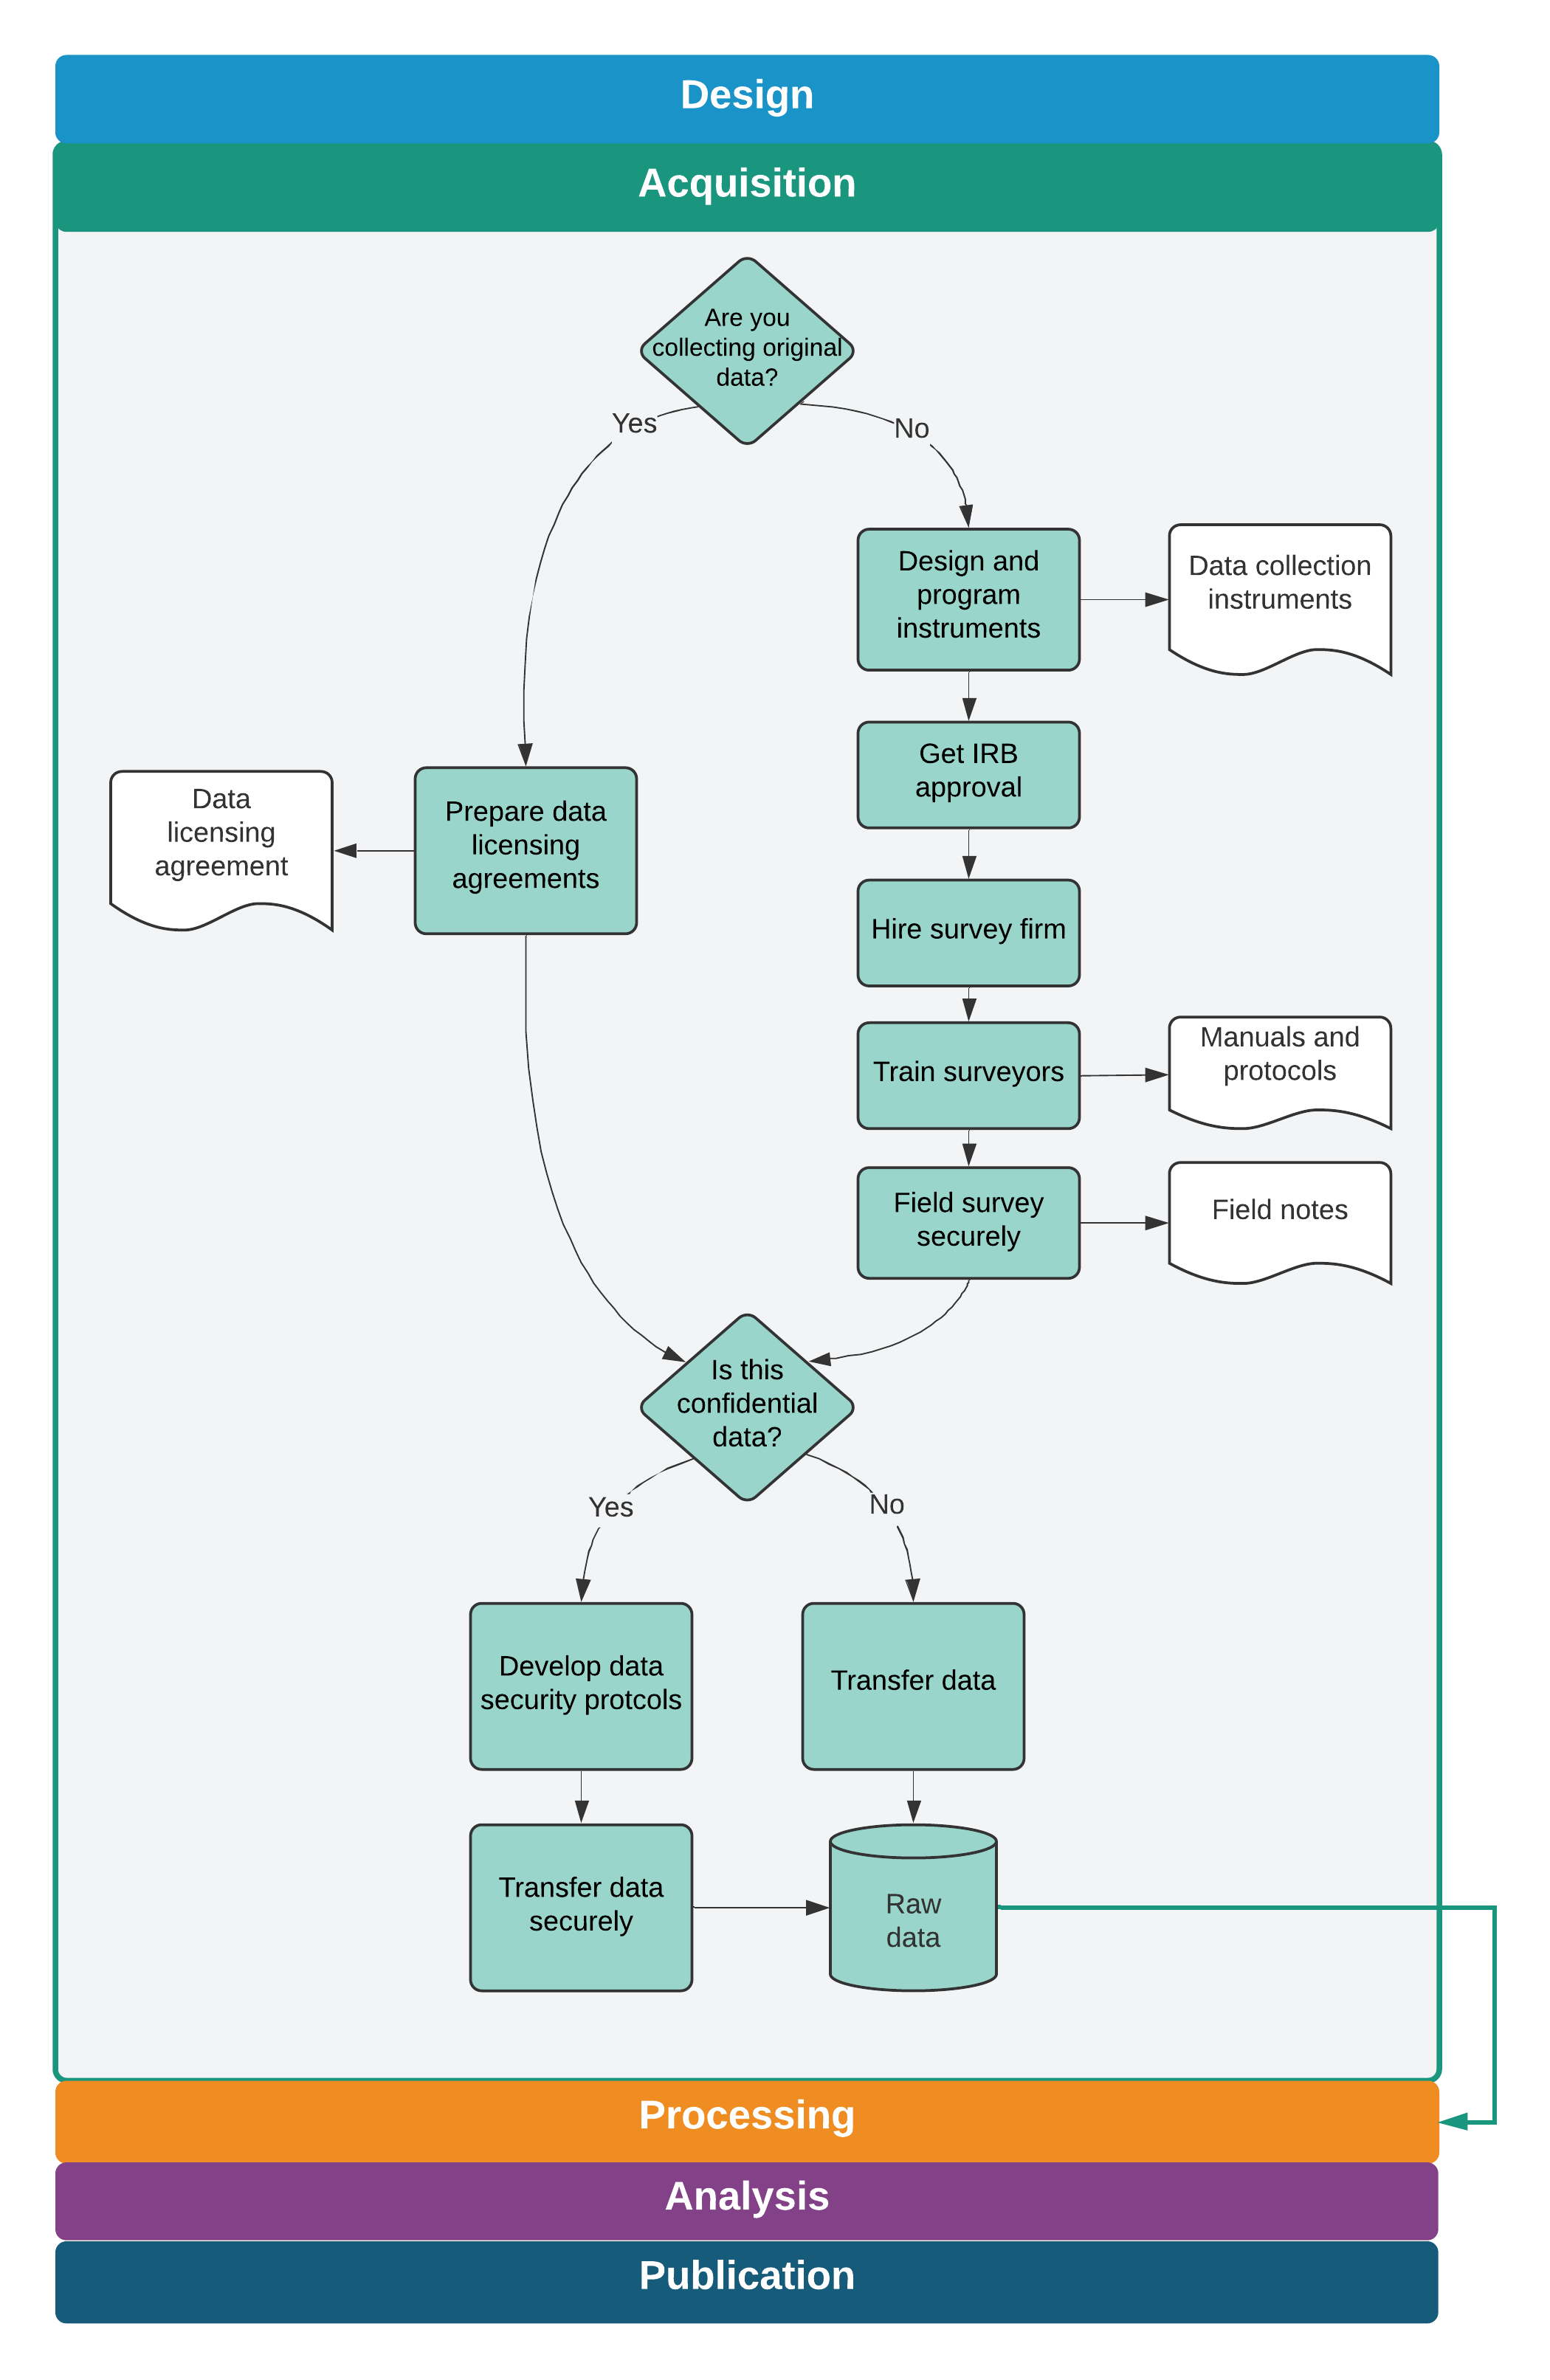
\includegraphics[width=1.5\linewidth]{diagrams/Acquisition}
		\caption{Data acquisition tasks and outputs}
	\end{figure}
\end{fullwidth}




%-------------------------------------------------------------------------------
%	CHAPTER 5
%-------------------------------------------------------------------------------

\chapter{Chapter 5: Cleaning and processing research data}
\label{ch:5}

%------------------------------------------------

\begin{fullwidth}

% What is data cleaning
Original data comes in a variety of formats,
most of which are not immediately suited for analysis.
The process of preparing data for analysis has many different names:
data cleaning, data munging, data wrangling.
But they all mean the same thing --
transforming raw data into a convenient format for your intended use.
This is the most time-consuming step of a project's data work,
particularly when primary data is involved;
it is also essential for data quality.
A structured workflow for preparing newly-acquired data for analysis
is essential for efficient, transparent, and reproducible data work.
One key point of this chapter is that no changes are made to the contents of data at this point.
We consider creating new variables, imputing values and correcting outliers
to be research decisions, and will discuss those in the next chapter.
Therefore, the clean dataset,
which is the main output from the workflow discussed in this chapter,
contains the same information as the raw data,
but in a format that is ready for use with statistical software.

% Chapter overview
This chapter describes the various tasks involved in making newly-acquired data ready for analysis.
The first section teaches you how to make your data \textit{tidy}.
This means adjusting how the dataset is organized
until the relationship between rows and columns is well-defined.
The second section describes quality assurance checks,
which are necessary to verify data accuracy.
The third section covers de-identification,
as removing direct identifiers early in the data handling process helps to ensure privacy.
The final section discusses how to examine each variable in your dataset and
make sure that it is as well documented and as easy to use as possible.
Each of these tasks is implemented through code,
and resulting datasets can be reproduced exactly by running this code.
The raw data files are kept exactly as they were acquired,
and no changes are made directly to them.

\end{fullwidth}

%------------------------------------------------


\section{Making data ``tidy''}

% Intro
The very first step in creating an analysis-friendly dataset
is understanding the data acquired,
and using this understanding to translate the data into an intuitive format.
This section discusses what steps may be needed to make sure that each row
in your \textbf{data tables}\sidenote{\textbf{Data table:}
	data that is structured into rows and columns.
	Also called \textit{tabular datasets} or \textit{rectangular data}.
	Examples of non-rectangular data are written text,
	NoSQL and graph databases, or files such as images.}
represents one observation.
Getting to such a format may be harder than expected,
and the \textbf{unit of observation}\sidenote{\textbf{Unit of observation:}
	the unit described by the data. In datasets, it is ideally what each row represents.
	More details on the concept of unit of observations
	can be found on the DIME Wiki:
  \url{https://dimewiki.worldbank.org/Unit_of_Observation}}\index{unit of observation}
 may be ambiguous in many raw datasets.
This section will present what we call a \textit{tidy} data format,
which is, in our experience, the ideal format to handle tabular data.
We will treat tidying data as the first step in data cleaning even though, in practice,
both tidying and quality monitoring should be done simultaneously as data is received.
This is because quality assurance can only be finalized using tidied data,
when it is guaranteed that each observation is uniquely identified.

%------------------------------------------------------------------------------
\subsection{Establishing a unique identifier}

% Uniquely and fully identifying variable
An important step before starting to tidy a dataset is
to understand the \textbf{unit of observation}
and find out which variable or set of variables
is the \textbf{unique identifier} for each observation.\sidenote{
	More details on the properties required for variables
	that uniquely identifies each observation
	can be found on the DIME Wiki:
  \url{https://dimewiki.worldbank.org/ID\_Variable\_Properties}}\index{unique identifier}
As discussed in Chapter 3,
the unique identifier will be used to link observations in this dataset
to data in other data sources according to the \textbf{data linkage table},\sidenote{
	More details on DIME's data linkage table template
	and an example can be found on the DIME Wiki:
	\url{https://dimewiki.worldbank.org/Data\_Linkage\_Table}}\index{data linkage table}
and the unique identifier for all observations
must be listed in the \textbf{master dataset}.\sidenote{
	More details on DIME's master dataset template
	and an example can be found on the DIME Wiki:
	\url{https://dimewiki.worldbank.org/Master\_Data\_Set}}\index{master dataset}
Ensuring that observations are uniquely and fully identified
is arguably the most important step in data cleaning.
It may be the case that the variables expected to uniquely identify
the raw data contain either missing or duplicate values.\sidenote{
	We use the expression \textbf{raw data}
	to refer to the ``data in the state it was originally received by the research team''.
 	In other sources, you will also see it used to refer to the
	``corrected and compiled dataset created from received information,
	reflecting only that information'',
	which we call \textbf{clean data}.
	This applies to data acquired from partners as well as
	original data collected by the research team.
}

It is also possible for a raw dataset to not include an unique identifier,
or that the identifier is not a suitable \textbf{project ID}.\sidenote{
	More details on what makes an ID variable
	a suitable Project ID variable
	can be found on the DIME Wiki:
	\url{https://dimewiki.worldbank.org/ID\_Variable\_Properties\#Project\_ID}}
Suitable project IDs should, for example, not involve long strings
that are difficult to work with, such as a name,
or be an ID that is known outside the research team.
In such cases, cleaning begins by
adding a project ID to the raw data.
If a project ID already exists,
for this unit of observation,
then you should carefully merge it
from the master dataset
to the raw data
using other identifying information.\sidenote{Such
	operations are commonly called ``merges'' in Stata, and
	``joins'' in R's \texttt{tidyverse} dialect.
	We will use the term \textit{merge} in this book.}
If a project ID does not exist,
then you need to generate one,
add it to the master dataset,
and then merge it back into the raw data.
Note that while digital survey tools create
unique identifiers for each data submission,
that is not the same as having a unique ID variable
for each observation in the sample,
as there can be multiple submissions
for the same observation.

DIME Analytics created an automated workflow to identify, correct and document
occurrences of duplicated entries in the unique identifier using
\texttt{ieduplicates} and \texttt{iecompdup},\index{ieduplicates}\index{iecompdup}
two Stata commands included in the \texttt{iefieldkit} package\index{iefieldkit}.
One advantage of using \texttt{ieduplicates}\sidenote{
	Read more about how to install and use \texttt{ieduplicates} and
	how the command can help you efficiently deal with duplicates
	on the DIME Wiki:
	\url{https://dimewiki.worldbank.org/ieduplicates}}
to correct duplicated entries is that it creates \textit{duplicates reports}
which records each corrections made and documents the reason for it.
Even if you are not using this command,
it is important to keep a record of all cases of duplicated IDs encountered
 and how they were resolved.

%-------------------------------------------------------------------------------
\subsection{Tidying raw data}

Though raw data can be acquired in all shapes and sizes,
it is most commonly received as one or multiple data tables.
These data tables can organize information in multiple ways,
and not all of them result in easy-to-handle datasets.
Fortunately, a vast literature of database management has identified the format
that makes interacting with the data as easy as it can be.
We call data in such format \textbf{tidy}.
A data table is tidy when each column represents one \textbf{variable},\sidenote{
  \textbf{Variable:} the collection of all data points
	that measure the same attribute for each observation.}
each row represents one observation,
and all variables in it have the same unit of observation.
Every other format is \textit{untidy}.
This may seem trivial, but raw data,
and raw survey data in particular,
is rarely received in a tidy format.

The most common case of untidy raw data encountered in development research
is a dataset with multiple units of observations stored in the same data table.
Take, for example, a household survey that includes household-level questions,
as well as a household member roster.
Such raw datasets usually consists of a single data table
where questions from the household member roster are saved in different columns,
one for each member, with a corresponding member suffix,
and household-level questions are represented by one column each.
When your rows include multiple nested observational units,
then the identifying variable does not identify all observations on that row,
as there is more than one unit of observation on the same row.

Survey data containing nested units of observation is typically
imported from survey platforms in \textbf{wide format}.\sidenote{\textbf{Wide data:}
	a data table where a single variable is divided into multiple columns,
	for example one for each individual in a household.}\index{wide data format}
Wide format data could have, for instance,
one column for a household-level variable (for example \texttt{ownsfridge}),
and a few columns for household member-level variables (for example \texttt{sex\_1}, \texttt{sex\_2}).
Raw data is often saved in this format because it's the most efficient way to transfer it:
adding different levels of observation into the same data table
allows for data to be transferred in a single file.
However, this leads to the widespread practice of interacting with data in wide format,
although doing so is often inefficient and error-prone.

To understand how dealing with wide data can be complicated,
imagine you need to calculate the share of women
in each household using the household level data described above.
In a wide data table you will either have to first create variables counting
the number of women and the total number of household members,
and then calculate the share,
or you will have to transform the data to a different format.
In a tidy data table, however, where each row is a household member,
you can easily aggregate the share of women by household,
without additional steps,
and then merge the result to the household-level data tables.
Tidy data tables are also easier to clean,
as each attribute only needs to be checked once,
and each column corresponds directly to one question in the questionnaire.
Finally, as you will see in Chapter 6,
summary statistics and distributions are much simpler
to generate from tidy data tables.

As mentioned earlier, there are unlimited ways for data to be untidy;
wide format is only one of those ways.
Another example is a data table containing both information on transactions
and on the firms involved in each transaction.
In this case, the firm-level information will be repeated
for all transactions a given firm was involved in.
Analyzing data in this format would give more weight
to firms that conducted more transactions,
which may not be consistent with the research design.

The basic process behind tidying a data table is simple:
first, identify all the variables that were measured at the same level of observation;
second, create separate data tables for each level of observation;
and third, reshape\sidenote{\textbf{Reshape:}
	transform a data table in such a way that the unit of observation represented by a row changes.}
the data and remove duplicated rows
until each data table is uniquely and fully identified by the identifying variable
that corresponds to its unit of observation.
Reshaping data tables is the most intricate task in data cleaning;
you should be very familiar with commands such as
\texttt{reshape} in Stata and \texttt{pivot} in R.
You must be sure that identifying variables are consistent across data tables,
so they can always be linked.
Reshaping is the type of transformation we referred to
in the example of how you calculate
the share of women in a wide data set.
The important difference is that
in a tidy workflow,
instead of transforming the data for each operation,
this transformation is done once for all data during cleaning,
making all subsequent operations much easier.

In the earlier household survey example,
household-level variables will be stored in one tidy data table,
and household-member variables are reshaped
and stored in a separate, member-level, tidy data table,
which also contains the household ID for each individual.
The household ID is intentionally duplicated in the household members data table
to allow one or several household members to be linked to the same household data.
The unique identifier for the household member-level data data will be
either a single household member ID or
a combination of household ID and household member ID.
In the transaction data example,
the result of the tidying process would be one transaction-level data table,
containing variables indicating the ID of all firms involved;
and one firm-level data table with a single entry for each firm.
Then, firm-level analysis is easily done
by calculating appropriate statistics in the transactions data table
(in Stata, often through \texttt{collapse})
and then merging or joining those results to the firms data table.

In a tidy workflow, your clean dataset is a set of one or more tidy data tables.
In both examples above, your clean dataset is made up of two tidy data tables.
There must be a clear way to connect each
tidy data table to a master dataset,
and thereby also to all other datasets.
To implement this, you need to decide which data table is the main data table;
that data table's unit of observation will be
the main unit of observation of your dataset.
The main unit of observation must directly correspond to a master dataset,
and be listed in the data linkage table.
All other data tables in your dataset must have
an unambiguous way to merge with the main data table.
This way, it will be possible to link
all data points in all your project's datasets to each other.
We recommend that you save your datasets as a folder,
in which the main data table shares the same name as the folder,
and the name of all other data tables start with the same name,
but are suffixed with the unit of observation for that data table.

In the household dataset example,
the household-level data table would be the main table.
This means that there must be a master dataset for households.
(You may have a master dataset for household members as well
if you think it is important for your research,
but it is not strictly required.)
The household data set would then be stored in a folder called,
for example, \texttt{baseline-hh-survey/}.
In that folder you would save both
the household-level data table with the same name as the folder,
for example \texttt{baseline-hh-survey.csv},
and the household member-level data named in the same format but with a suffix,
for example \texttt{baseline-hh-survey-hhmember.csv}.

The tidying process gets more complex as the number of nested groups increases.
That means the steps of identifying the unit of observation of each variable
and reshaping the separated data tables need to be repeated multiple times.
However, the more nested groups a dataset includes,
the more efficient it is to deal with tidy data as compared to untidy.
Cleaning and analyzing wide datasets, in particular,
is a repetitive and error-prone process.

The next step of data cleaning, data quality monitoring,
may involve comparing different units of observation.
Aggregating sub-units to compare to a higher unit is much easier with tidy data,
which is why we suggest tidying data as the first step in the cleaning workflow.
If you are conducting primary data collection,
you can start preparing or coding the data tidying even before the data is acquired,
since you will know in advance the exact format in which the data will be received.
In the case of survey data,
tidying datasets will guarantee a one-to-one correspondence
between questions in the questionnaire and columns in the data.
Preparing the data for analysis, the last task in this chapter,
is much simpler when that is the case.

%------------------------------------------------
\section{Assuring data quality}

% Intro
Whether you are acquiring data from a partner or collecting it directly,
it is important to make sure that data faithfully reflects ground realities.
You should carefully examine and clean any data you are about to use.
When reviewing raw data, you will inevitably encounter data entry mistakes,
such as typos and inconsistent values.
Whether your team is conducting a survey or
you are receiving administrative data from a partner,
the key aspects to have in mind are
data completeness, consistency and distribution.
Data quality assurance checks should be performed as soon as the data is acquired.
When data is being collected and transferred to the team in real-time,
this means conducting high-frequency checks.
Primary data require extra attention to quality checks,
as data entry by humans is more susceptible to errors,
and the research team will be the only line of defense between
data issues and the data analysis.
Survey-specific quality monitoring protocols are discussed in Chaper 4.

\subsection{Implementing data quality checks}
% Why they should be made in real-time
Data quality checks should carefully inspect key treatment and outcome variables
to ensure that the data quality of core study variables is uniformly high,
and that additional effort is centered where it is most important.
They should be run every time data is received
to flag irregularities in the acquisition progress, in sample completeness, or in response quality.
The faster issues are identified, the more likely they are to be solved.
Once the field team has left a survey area,
or high-frequency data has been deleted from a server,
it may be impossible to verify whether data points are correct or not.
Even if the research team is not receiving data in real-time,
the data owners may not be as knowledgeable about the data,
or even as responsive to the research team queries, as time goes by.
\texttt{ipacheck}\sidenote{
	\url{https://github.com/PovertyAction/high-frequency-checks}}
is a very useful Stata command that automates some of these tasks,
regardless of the data source.

% Completeness
It is important to check continuously that the observations received match the intended sample.
In surveys, electronic survey software often provides case management features
through which sampled units are directly assigned to individual enumerators.
For data received from partners, such as administrative data,
this may be harder to validate.
In these cases, cross-referencing with other data sources can help to ensure completeness.
It is often the case that raw data includes duplicate or missing entries,
which may occur due to typos, failed submissions to data servers,
or other mistakes.\sidenote{
  More details on how to deal with duplicates during surveys
	and how to track completion
	can be found on the DIME Wiki:
	\url{https://dimewiki.worldbank.org/Duplicates_and_Survey_Logs}}
Issues with data transmission often result in missing observations,
particularly when large datasets are being transferred,
or when data is being collected in locations with limited internet connection.
Keeping a record of what data was submitted,
and comparing it to the data received as soon as transmission is complete
reduces the risk of noticing that data is missing when it is no longer possible to recover it.

% match to sample
Once data completeness is confirmed,
observed units must be validated against the expected sample:
this is as straightforward as merging the sample list
with the data received and checking for mismatches.
Reporting errors and duplicate observations in real time allows for efficient corrections.\sidenote{
	Read more about how to install and use \texttt{ieduplicates} and
	how the command can help you efficiently deal with duplicates
	on the DIME Wiki:
	\url{https://dimewiki.worldbank.org/ieduplicates}}\texttt{ieduplicates}
provides a workflow for resolving duplicate entries with the data provider.
For surveys, it is also important to track data collection progress to  monitor attrition,
so that it is clear early on if a change in protocols or additional tracking will be needed.\sidenote{
  See \citet{ozler2016combining} for an example.}
Remember to also check survey completion rates
and sample compliance by surveyors and survey teams,
and compare data missingness across administrative regions,
to identify any clusters that may be providing data of suspect quality.

% Consistency
Quality checks should also include checks of response quality and consistency.
For example, whether the values for each variable fall within the expected range,
and related variables do not contradict each other.\sidenote{
  More details about real-time data quality assurance
  and links to additional resources
  can be found on the DIME Wiki:
  \url{https://dimewiki.worldbank.org/Monitoring_Data_Quality}}
Electronic data collection systems often incorporate many quality control features,
such as range restrictions and logical flows.
Data received from systems that do not include such controls should be checked more carefully.
Consistency checks are project specific, so it is difficult to provide general guidance.
A detailed knowledge of the variables in the dataset and a careful examination of the analysis plan
is the best way to prepare.
Examples of inconsistencies in survey data would include cases where
a household reports having cultivated a plot in one module,
but does not list any cultivated crops in another.
Response consistency should be checked across all datasets, as this is much harder to automate.
For example, if two sets of administrative records are received,
one with hospital level information and one with data on each medical staff,
the number of entries in the second set of entries should match
the number of employed personnel in the first one.

% Distribution
Finally, no amount of pre-programmed checks can replace actually looking at the data.
Of course that doesn't mean eye checking each data point,
but rather plotting and tabulating distributions for your main variables of interest.
This will help you identify outliers and
other potentially problematic patterns that you had not foreseen.
A common source of outliers values in survey data are typos,
but they can also occur in admin data if, for example,
the unit reported changed over time,
but the data was stored with the same variable name.
Identifying unforeseen patterns in the distribution will also help you gather relevant information,
for example whether there was no harvest data because of a particular pest in the community
or if the unusual call records in a particular area caused by temporary downtime of a tower.
Analysis of metadata and paradata can also useful in assessing data quality.
For example, electronic survey software generates
automatically collected timestamps and trace histories,
showing when data was submitted, how long enumerators spent on each question,
and how many times answers were changed before or after the data was submitted.

\section{Processing confidential data}

When implementing the steps discussed up to this point,
you are likely to be handling confidential data.
Effective data quality monitoring
frequently requires you to identify the individual observations in your dataset,
and the people or other entities who provided the information.
Using identified data allows you to quickly follow up on and resolve identified issues.
Handling confidential data such as
\textbf{personally-identifying information}\index{personally-identifying information}
requires a secure environment and, typically, decryption.
De-identifying the data will allow you to simplify that workflow,
and will also reduces the risk of harmful leaks.
This section describes how to de-identify data in order to share it with a wider audience.

\subsection{Protecting research subject privacy}

% Dealing with human subjects
Most development data involves human subjects.\sidenote{
    Read more about what extra consideration
	you must take into account when
	working with human subjects on the DIME Wiki:
	\url{https://dimewiki.worldbank.org/Protecting_Human_Research_Subjects}}
\index{human subjects}
As a researcher, you may have access to personal information about your subjects:
where they live, how much income they have,
whether they have committed or been victims of crimes,
their names, their national identity numbers, and other sensitive data.\sidenote{
  See \citet{banerjee2019entertainment} for an example.}
There are strict requirements for safely storing and handling personally-identifying data,
and it is the responsibility of the research team to satisfy these requirements.\sidenote{
  More details on research ethics as well as links to tools and
  other resources related can be found on the DIME Wiki:
	\url{https://dimewiki.worldbank.org/Research\_Ethics}.
  It can also be found under Pillar 1 in the DIME Research Standards:
  \url{https://github.com/worldbank/dime-standards}}
Everyone working with human subjects research should
have completed an ethics certification course.\sidenote{
  Protecting Human Research Participants (\url{https://phrptraining.com})
  and the CITI Program (\url{https://citiprogram.org})
  are common options.}
A plan for secure data handling is typically also required for IRB approval.

% Options for dealing with PII data: only collect it if extremely necessary, encrypt it, restrict access, de-identify it
The best way to avoid risk is to minimize interactions with PII as much as possible.
First, only collect personally-identifying information that is strictly necessary for the research.
Second, avoid the proliferation of copies of identified data.
There should never be more than one copy of the raw identified dataset in the working project folder,
and it must always be encrypted.
Third, de-identify the data as early as possible in the workflow.
Even within the research team,
access to the identified data should be limited to team members who require it for their specific tasks.
Data analysis that requires identifying information is rare
and in most cases can be avoided by properly linking masked identifiers to research information
such as treatment statuses and weights, then removing unmasked identifiers.

% De-identification vs anonymization
Once data is acquired and the data quality checks described above are completed,
the next task is typically to \textbf{de-identify} the data,
by removing or masking all personally-identifying variables.\sidenote{
	More details and best practices related to de-identification
	as well as tools that can help you assess disclosure risks
	can be found on the DIME Wiki:
	\url{https://dimewiki.worldbank.org/De-identification}}
\index{de-identification}
Note that it is in practice impossible to \textbf{anonymize} data.
There is always some statistical chance that an individual's identity
will be re-linked to the stored data
-- even if that data has had all directly identifying information removed --
by using some other data that becomes identifying when integrated.
For this reason, we typically recommend de-identification in two stages.
The \textbf{initial de-identification} process,
performed as soon as data is acquired, strips the data of direct identifiers,
to create a working de-identified dataset that
can be shared \textit{within the research team} without the need for encryption.
The \textbf{final de-identification} process,
performed before data is publicly released, involves
careful consideration of the trade-offs between
risk of identifying individuals and the utility of the data,
and typically requires the removal of a further level of indirect identifiers.
The rest of this section describes how to implement
both the initial and the final de-identification processes.

\subsection{Implementing de-identification}

% Initial de-identification
Initial de-identification reduces risk and simplifies workflows.
Once you create a de-identified version of the dataset,
you no longer need to interact directly with the encrypted data.
Note that if the data tidying resulted in multiple raw data tables,
each will need to be de-identified separately, but
the workflow will be the same for all of them.

During the initial round of de-identification,
datasets must be stripped of personally identifying information.
To do so, you will need to identify all variables that contain such information.
For data collection, where the research team designs the survey instrument,
flagging all potentially identifying variables at questionnaire design stage
simplifies the initial de-identification process.
If you did not do that, or you received original data by another means,
there are a few tools to help flag variables with personally-identifying data.
JPAL's \texttt{PII-scan} and
IPA's \texttt{PII\_detection},
scan variable names and labels for common string patterns
associated with identifying information.\sidenote{
	\url{https://github.com/J-PAL/PII-Scan} and
	\url{https://github.com/PovertyAction/PII\_detection}}
The World Bank's \texttt{sdcMicro}
lists variables that uniquely identify observations,
but its more refined method and
higher processing capacity requirement makes it
better suited for final de-identification.\sidenote{\citet{benschop2019statistical}}
The \texttt{iefieldkit} command \texttt{iecodebook}
lists all variables in a dataset and exports an Excel sheet
where you can easily select which variables to keep or drop.\sidenote{
  Read more about how to install and use \texttt{iecodebook} and
	how the command can help in de-identification and other cleaning tasks
	on the DIME Wiki:
	\url{https://dimewiki.worldbank.org/iecodebook}}

% Initial de-identification in practice
Once you have a list of variables that contain confidential information,
assess them against the analysis plan and first ask yourself for each variable:
\textit{will this variable be needed for the analysis?}
If not, the variable should be dropped.
Don't be afraid to drop too many variables the first time,
as you can always go back and extract additional variables from the raw data,
but you cannot go back in time and drop a PII variable that was leaked.

For each confidential variable that is needed in the analysis, ask yourself:
\textit{can I encode or otherwise construct a variable that masks the confidential component, and
	then drop this variable?}
For example, it is easy to encode identifiers for small localities like villages
and only provide a meaningless numerical indicator
showing which observations are in the same village
without revealing which villages are included in the data.
This is typically the case for most identifying information.
If the answer to either of the two questions above is yes,
all you need to do is write a script to drop the variables that are not required for analysis,
encode or otherwise mask those that are required,
and save a working version of the data.
For example:
after constructing measures of distance or area,
drop the specific geolocations in the data;
after constructing and verifying numeric identifiers in
a social network module, drop all names.
If confidential information is strictly required for the analysis and cannot be
masked or encoded,
then at least the confidential part of the data is required
to remain encrypted
and only be decrypted when used during in the data analysis process.
Using confidential data in the analysis process
does \textit{not} justify storing or sharing it in an insecure way.

% Final de-identification: sdcMicro
After initial de-identification is complete,
your dataset will consist of one or multiple tidy,
de-identified data tables.
This is the dataset that you will interact with
during the remaining tasks described in this chapter.
Initial de-identification should not affect the usability of the data.
Note that access to the initially de-identified data
should still be restricted to the research team only,
as indirect identifiers may still present a high risk if disclosure.
It is common, and even desirable, for teams to make data publicly available
once the tasks discussed in this chapter are concluded.
This will allow other researchers to conduct additional analysis and to reproduce your finding.
Before that can be done, however,
you should further consider whether your data can be re-identified,
in a process we call \textbf{final de-identification},
which will be discussed in more detail in Chapter 7.


\section{Cleaning and preparing data for analysis}

% What is data cleaning
The last step in the data cleaning process involves
making the dataset easy to use and understand, and
carefully examining each variable to document distributions
and identify patterns that may bias the analysis.
The resulting dataset will contain only the variables collected in the field, and
no modifications to data points will be made,
except for corrections of mistaken entries.
You may have more data tables in your dataset now then originally received,
and they may have a different \textit{format},
but the information contained is still the same.
Apart from the \textbf{cleaned dataset} (or datasets) itself,
cleaning will also yield extensive documentation describing it.

% Section overview
Data cleaning yields in-depth understanding of the contents and structure of your data.
This knowledge will be key to correctly constructing and analyzing final indicators,
which we cover in the next chapter.
Do not rush through this step!
It is common for data cleaning to be the most time-consuming task in a project.
In this section, we introduce some concepts and tools to make it more efficient and productive.
The section is separated into three subtopics:
exploring the data, making corrections, and recoding and annotating.
They are separated here because they are different in nature,
and should be kept separated in your code.
In practice, however, they may all done at the same point in time.


\subsection{Exploring the data}

% What to look for when exploring the data
The first time you interact with the data contents is during quality checks.
However, these checks are are usually time-sensitive,
and there may not be time to explore the data at length.
During data cleaning, on the other hand,
you will need to inspect each variable closely.
Use tabulations, summary statistics, histograms and density plots to understand the structure of data,
and look for patterns or irregularities.
Think critically about what you see.
You should ensure that the numerical values that appear
are consistent with the information the variable represents.
You should ensure that statistical distributions look realistic
and are not highly clumped or skewed.
You should confirm that related variables are consistent with each other.
You should check for outliers and missing values.
Then, you should assess if unusual or unexpected distributional patterns
of any of these characteristics could be caused by data entry errors.

% Document patterns rather than fix them
At this point, it is more important to document your findings
than to directly address any irregularities found.
There is a very limited set of changes that should be made to the raw data during cleaning.
They are described in the next two sections,
and are usually applied to each variable as you examine it.
Most of the transformations that result in new variables
will be done during \textbf{data construction},\sidenote{
  \textbf{Data construction:} The process of creating complex or abstract measures
  from raw information that is directly observed or collected.}\index{data construction}
a process discussed in the next chapter.
For now, focus on creating a record of what you observe,
and extensively documenting the data being explored.
You will use this documentation when discussing with your team
how to address irregularities once you get to the construction stage.
This material will also be valuable during exploratory data analysis.

\subsection{Correcting data points}

% Correct or not correct
As mentioned earlier,
corrections to issues identified during data quality monitoring are
the only changes done to individual data points during the data cleaning stage.
However, there is a lot of discussion about whether one should modify such data points at all.
Some argue that follow-ups to the issues identified are costly and add limited value.
Since it is not possible to check each and every possible data entry error,
doing so can create a false sense of security from issues identified on a few main variables.
Additionally, manually-inspected data may suffer from considerable inspector variability.
In many cases, the main purpose of data quality checks
is to detect fraud and identify problems with data collection protocols.
On the other hand, there is also an argument to be made
against keeping clear typing errors or not correcting missing values.
We recommend correcting any entries that are clearly identified as errors.
However, there is some subjectivity involved in deciding
which cases fall into this category.
A common rule of thumb is to include the set of corrections
which are based on information that you have privileged access to
and other research teams would not be able to make, and no more.
Making this such decisions involve deep knowledge of the data and
the particular circumstances or each research project.

% Documentation
Whether you decide to modify your data or not,
you must keep a careful record of all issues that you identify.
If no data points are modified,
it may still be helpful to add flags to observations containing
potentially problematic values,
so you can verify how they affect results during analysis.
If your team decides to follow up on and correct these issues,
the follow-up process must also be thoroughly documented.
Be very careful not to include confidential information in documentation that is not securely stored,
or that you intend to release as part of a replication package or data publication.
Finally, remember not to make changes directly to the raw data.
Instead, any corrections must be done as part of data cleaning,
applied through code, and saved to a new intermediate dataset.

\subsection{Recoding and annotating data}

% Why recoding and annotating data are important
The cleaned dataset is the starting point of data analysis.
It will be extensively manipulated to construct analysis indicators,
so it is important for it to be easily processed by statistical software.
To make the analysis process smoother,
anyone opening this dataset for the first time should have all the information needed to interact with it,
even if they were not involved in the acquisition or cleaning process.
This will save them time going back and forth between the dataset and its accompanying documentation.

% Encoding variables
Often times, datasets are not imported into statistical software in the most efficient format.
The most common example is string (text) variables:
categorical variables and open-ended responses are often read as strings.
However, variables in this format cannot be used for quantitative analysis.
Therefore, categorical variables must be transformed into other formats,
such as \texttt{factors} in R and \texttt{labeled integers} in Stata.\sidenote{
  More details on value labels in Stata
	and best practices on how to work with them
	can be found on the DIME Wiki:
	\url{https://dimewiki.worldbank.org/Data\_Cleaning\#Value\_Labels}}
Additionally, open-ended responses stored as strings usually have a high risk of including identifying information,
so cleaning them requires extra attention.
The choice names in categorical variables
(called \textit{value labels} in Stata and \textit{levels} in R)
should be accurate, concise,
and directly linked to the data collection instrument.
Adding choice names to categorical variables
makes it easier to understand your data as you explore it,
and thus reduces the risk of small errors making their way through into the analysis stage.

% Recoding missing values
In survey data, it is common for non-responses such as ``Don't know'' and ``Declined to answer''
to be represented by arbitrary survey codes.
The presence of these values could bias your analysis,
since they don't represent actual observations of an attribute.
They need to be turned into \textit{missing values}.
However, the fact that a respondent didn't know how to answer a question is also useful information
that would be lost by simply omitting all information.
In Stata, this information can be elegantly conserved using extended missing values.\sidenote{
	More details on survey codes
	and how they relate to best practices when working with missing values in Stata
	can be found on the DIME Wiki:
	\url{https://dimewiki.worldbank.org/Data\_Cleaning\#Survey\_Codes\_and\_Missing\_Values}}

% Labeling variables
We recommend that the cleaned dataset be kept as similar to the raw data as possible.
This is particularly important regarding variable names:
keeping them consistent with the raw data makes data processing and construction more transparent.
Unfortunately, not all variable names are informative.
In such cases, one important piece of documentation
 makes the data easier to handle: the variable dictionary.
When a data collection instrument (for example a questionnaire) is available,
it is often the best dictionary one could ask for.
But even in these cases, going back and forth between files can be inefficient,
so annotating variables in a dataset is extremely useful.
In Stata, \textit{variable labels}\sidenote{
	More details on variable labels in Stata
	and best practices on how to work with them
	can be found on the DIME Wiki:
	\url{https://dimewiki.worldbank.org/Data\_Cleaning\#Variable\_Labels}}
must always be present in a cleaned dataset.
They should include a short and clear description of the variable.
A lengthier description, that may include, for example,
the exact wording of a question, may be added through \textit{variable notes}.
In R, it is less common to use variable labels,
and a separate dataset with a variable dictionary is often preferred,
but \texttt{data frame attributes} can be used for the same purpose.

% Dropping irrelevant variables
Finally, any information that is not relevant for analysis may be removed from the dataset.
In primary data, it is common to collect information for quality monitoring purposes,
such as notes, duration fields and surveyor IDs.
Once you are past the quality monitoring phase,
these variables may be removed from your dataset.
In fact, to make the data easier to handle,
you may choose to start from a minimal set of variables,
and add new ones as you clean them.
To ensure the cleaned dataset file doesn't get too big to be handled,
use commands such as \texttt{compress} in Stata so the data
is always stored in the most efficient format.

% Cleaning tools: iecodebook, tidyverse
Although all these tasks are key to making the data easy to use,
implementing them can be quite repetitive and create convoluted scripts.
The \texttt{iecodebook} command suite, part of the \texttt{iefieldkit} Stata package,
is designed to make some of the most tedious components of this process more efficient.\sidenote{
  Read more about how to install and use \texttt{iecodebook} and
	how the command can help making cleaning tasks more efficient
	on the DIME Wiki:
	\url{https://dimewiki.worldbank.org/iecodebook}}
\index{iecodebook}\index{iefieldkit}
It also creates a self-documenting workflow,
so your data cleaning documentation is created alongside that code,
with no extra steps.
As far as we know, currently there are no similar resources in R.
However, the \texttt{tidyverse}\sidenote{\url{https://www.tidyverse.org/}} packages
compose a consistent and useful grammar to perform the same tasks.

%--------------------------------------------------------------
\subsection{Documenting data cleaning}

Throughout the data cleaning process,
you will often need extensive inputs from the people responsible for data collection.
Sometimes this is your research team, but often it will be someone else.
It could be a survey team, the government ministry responsible for administrative data systems,\sidenote{
  See \citet{fernandes2015trade} for an example.}
the technology firm that generated remote sensing data, etc.
Regardless of who originally collected the data,
you should acquire and organize all documentation of how the data was generated.\sidenote{
  More details on how to best document your data and
	links to additional resources on this topic can be found on the DIME Wiki:
	\url{https://dimewiki.worldbank.org/Data\_Documentation}}\index{documentation}
What type of documentation that is available depends on how the data was collected.
For original data collection, this should include
field protocols, data collection manuals, survey instruments,
supervisor notes, and data quality monitoring reports.
For secondary data, you should try to get the same type of information,
but that is often not possible unless
the data source is a well managed data publication.
Independently of its exact composition,
the data documentation should be stored
alongside your data dictionary and codebooks.
You will probably need these files during analysis,
and they should be published along with the data,
so other researchers may use them for their analysis as well.

\section{Looking ahead}
This chapter introduced a workflow of formatting, cleaning, and quality assurance for
the data that you obtained from the field or from partners,
illustrated in the figure that follows.
These tasks create your first research outputs using original data:
an analysis-ready dataset.
This dataset is well-structured to describe your units of analysis (it is ``tidy''),
it faithfully represents the measurements it was intended to collect,
and it does not expose the identities of the people described by it.
You have also now taken the time to fully understand the patterns and structures
in your data, and annotated and labeled them for your use and use by others.
Combined with the data map, this dataset
will be the fundamental starting point for all analysis work.
In the next chapter, we will walk through the steps needed
to run the analyses originally specified in your analysis plan
and answer your research question --
or perhaps to find out you now have even more questions.

\begin{fullwidth}
	\begin{figure}
		\centering
		\includegraphics[width=1.6\linewidth]{diagrams/Cleaning}
		\caption{Data processing input, tasks, and outputs}
		\label{fig:cleaning}
	\end{figure}
\end{fullwidth}

%--------------------------------------------------------------


%-------------------------------------------------------------------------------
%	CHAPTER 6
%-------------------------------------------------------------------------------

\chapter{Chapter 6: Constructing and analyzing research data}
\label{ch:6}

%------------------------------------------------

\begin{fullwidth}

% Intro ----------------------------------------

% Motivation

The process of data analysis is typically
a back-and-forth discussion between people
with differing skill sets.
To effectively do this in a team environment,
data, code and outputs must be well-organized and documented,
with a clear system for version control,
analysis scripts that can be run by all team members,
and creation of research outputs fully automated.
Putting in time upfront to structure the data analysis workflow
in a reproducible manner pays substantial dividends throughout the process.
Similarly, documenting research decisions made during data analysis
is essential not only for research quality and transparency,
but also for the smooth implementation of a project.

% Chapter overview
In this chapter, we discuss the necessary steps to transform
cleaned raw data into informative analysis outputs such as tables and figures.
The suggested workflow starts where the last chapter ended:
with the outputs of data cleaning.
The first section covers variable construction:
transforming the raw data into economically meaningful indicators.
The second section discusses the analysis code itself.
We do not offer instructions on how to conduct specific analyses,
as that is determined by research design,
and there are many excellent existing guides.
Rather, we discuss how to structure and document data analysis
that is easy to follow and understand,
for both the full research team members and research consumers.
The final section discusses ways to automate common outputs
so that your work is fully reproducible.

\end{fullwidth}

%------------------------------------------------

\section{Creating analysis datasets}

% What is construction
For this chapter, we assume you are starting from
one or multiple well-documented tidy\sidenote{\citet{hadley2017R}} datasets.
We also assume that these datasets
have gone through thorough quality checks
and incorporate any corrections needed.\sidenote{
	See chapter 5 for discussions on how to
	tidy data, monitor data quality and document corrections.
}
The next step is to \textbf{construct}\sidenote{
	\textbf{Data construction}:
	The process of transforming cleaned data into analysis data by
	creating the derived indicators that will be analyzed.}
the variables that you will use for analysis;
that is, to transform the cleaned data into analysis-ready data.
It's possible the data is ready for analysis as acquired,
but in most cases it needs to be prepared by integrating different datasets
and creating derived variables
(dummies, indices, and interactions, to name a few\sidenote{
  See \citet{adjognon2019reducing} for an example.}).
The derived indicators you will construct should be
planned during research design\index{research design},
with the pre-analysis plan serving as a guide.\index{pre-analysis plan}
During construction, data will typically be
reshaped, merged, and aggregated to change the level of the data points
from the \textbf{unit of \textit{observation}} in the raw data
to the \textbf{unit of \textit{analysis}}.\sidenote{
	More details on the concepts of unit of observations
	and unit of analysis
	can be found on the DIME Wiki:
	\url{https://dimewiki.worldbank.org/Unit\_of\_Observation}}
\index{unit of observation}\index{unit of analysis}

% A project may require multiple purpose-built data sets
Each analysis dataset is built to answer an analysis question.
If the sub-samples and units of observation
vary for different pieces of the analysis,
you will probably need to create many purpose-built analysis datasets.\index{analysis datasets}
In such cases, it is not good practice
to try to create a single ``one-size-fits-all'' analysis dataset.
For a concrete example of what this means,
think of an agricultural intervention
that was randomized across villages
and only affected certain plots within each village.
The research team may want to
run household-level regressions on income,
test for plot-level productivity gains,
and check if village characteristics are balanced.
Having three separate datasets for each of these three pieces of analysis
will result in cleaner, more efficient, and less error-prone analytical code than if
you started from a single analysis dataset and repeatedly transformed it.

\subsection{Organizing data analysis workflows}

% Why construction is separate from data cleaning
Construction follows data cleaning and
should be treated as a separate task for two reasons.
First, this helps to clearly differentiate error corrections
(necessary for all data uses)
from creation of analysis indicators
(necessary only for specific analyses).
Second, it helps to ensure that variable definitions are
consistent across datasets.
For example, take a project that has a baseline and an endline survey.
Unless the two data collection instruments are exactly the same,
which is preferable but often not the case,
the data cleaning for each of these rounds will require different steps,
and therefore will be done separately.
However, the analysis indicators must be constructed in the exact same way,
so they are comparable.
To do this, you will require at least two separate cleaning scripts,
and a unified construction script.
Maintaining one construction script guarantees that you will not
accidentally make changes to an indicator from one round
while forgetting to update the other.

% Why construction is separate from analysis
When we visualize the research workflow,
variable construction precedes data analysis,
as derivative variables need to be created before they are analyzed.
In practice, however, as you analyze the data,
it is often useful to revisit construction,
and explore different subsets and transformations of the data.
Even if construction and analysis are done concurrently,
you should always code them in separate scripts.
If every script that creates a table starts by loading a dataset,
subsetting it, and manipulating variables,
any edits to construction need to be replicated in all scripts.
This increases the chances that at least one of them
will have a different sample or variable definition.
Coding all variable construction and data transformation
in a unified script, separate from the analysis code,
prevents such problems and ensures consistency across different outputs.

\subsection{Integrating multiple data sources}

% When merging is necessary and how to start thinking about it
To create the analysis dataset,
it is typically necessary to combine information
from different data sources
or different datasets with a common source.
For the next few paragraphs,
we call such operations ``merges'',
but they are also commonly referred to as ``data joins''.
As discussed in Chapter 3,
this process should be documented
using \textbf{data flowcharts},\sidenote{
	More details on DIME's data flow chart template
	and an example can be found on the DIME Wiki:
	\url{https://dimewiki.worldbank.org/Data\_Flow\_Charts}}
and different data sources should only be combined
in accordance with the data linkage table.\sidenote{
	More details on DIME's data linkage table template
	and an example can be found on the DIME Wiki:
	\url{https://dimewiki.worldbank.org/Data\_Linkage\_Table}}
For example, you may merge administrative data with survey data
in order to include demographic information in your analysis,
or you may want to integrate geographic information
in order to include location-specific controls.
To understand how to perform such operations,
you will need to consider the unit of observation for each dataset,
and their respective identifying variables.
Merges are frequent and complex operations,
which makes them a common source of error.
Whichever statistical software you are using,
take the time to read through the help file of merge commands
and make sure you understand their options and outputs.\index{merging data}

% How to think about merges
When writing the code to implement merge operations,
a few steps can help avoid mistakes.
First, before writing code to combine the datasets,
write pseudocode to understand which observations you expect to be
matched or not, and why.
When possible, determine exactly which and how many
matched and unmatched observations should result from the merge.
The best tool you have to understand this is
the three components of the data map discussed in chapter 3.
Second, think carefully about whether you want to keep matched and unmatched observations,
or only specific matching outcomes (e.g. to create a balanced panel),
and add that to the pseudocode as well.
Finally, run the code to merge the datasets,
and compare the outcome to your expectations.
Add comments to explain any exceptions,
and make it so the code will return an error in case unexpected results show up in future runs.

% Common mistakes
To avoid unintentional changes to your data,
pay close attention to merge results.
Two that require careful scrutiny are missing values and dropped observations.
Make sure to read about how each command treats missing observations:
are unmatched observations dropped, or are they kept with missing values?
Whenever possible, add automated checks in the script that throw an error message
if the result is different than what you expect,
or you may not notice changes in the outcome after running large chunks of code.
Document changes to the number of observations in your comments,
and explain why they are happening.
If your are subsetting your data by keeping only matched observations,
write down the reason why the observations differ across datasets,
as well as why you are only interested in those that matched.
The same applies when you are adding new observations from the merged dataset.

% Data integration
Some merges of data with different units of observation
are more conceptually complex.
Examples include: overlaying road location data with household data,
using a spatial match; combining school administrative data, such as attendance records and test scores,
with student demographic characteristics from a survey;
or linking a dataset of infrastructure access points, such as water pumps or schools,
with a dataset of household locations.
In these cases, a key part of the research contribution is figuring out
a useful way to combine the datasets.
Since the conceptual constructs that link observations from the two data sources
are important and can take many possible forms,
it is especially important for the data integration to not be treated mechanically,
and to be extensively documented, separately from other data construction tasks.


\subsection{Creating analysis variables}

% Main points to keep in mind for new variables
Once you have assembled variables from different sources into a single working dataset
with the right raw information and observations,
it's time to create the derived indicators of interest for analysis.\index{analysis variables}
Before constructing new indicators,
you must check and double-check units, scales, and value assignments of each variable that will be used.
This is when you will use the knowledge
of the data and the documentation developed during cleaning the most.
First, check that all categorical variables have the same value assignment,
such that labels and levels have the same correspondence across variables that use the same options.
For example, it's possible that in one question \texttt{0} means ``no'' and \texttt{1} means ``yes'',
while in another one the same answers were coded as \texttt{1} and \texttt{2}.\index{binary variables}
(We recommend coding binary questions as either \texttt{1} and \texttt{0} or \texttt{TRUE} and \texttt{FALSE},
so they can be used numerically as frequencies in means and as dummies in regressions.
This often implies re-expressing categorical variables like \texttt{gender} as binary variables like \texttt{woman}.)
Second, make sure that any numeric variables you are comparing
are converted to the same scale or unit of measure:
you cannot add one hectare and two acres and get a meaningful number.
New variables should be assigned functional names,
and the dataset ordered such that related variables are together.
Adding notes to each variable will make your dataset more user-friendly.

% Dealing with outliers and missing values
At this point, you will also need to decide
how to handle any outliers or unusual values identified during data cleaning.
How to treat outliers is a research question.\sidenote{
  For more details on how to deal with outliers
  see the DIME Wiki:
  \url{https://dimewiki.worldbank.org/Variable_Construction\#Dealing_with_outliers}}\index{outliers}
There are multiple possible approaches,
and the best choice for a particular case
will depend on the objectives of the analysis.
Whatever your team decides, make sure to explicitly note
what the decision was and how it was made.
Results can be sensitive to the treatment of outliers,
so keeping the original variable in the dataset
will allow you to test how much it affects your outputs.
All these points also apply to imputation of missing values and other distributional patterns.
As a general rule, never overwrite or delete original data during the construction process.
Always create derived indicators with new names.

% Dealing with different levels of observation
Two features of data create additional complexities when constructing indicators:
research designs comprising multiple units of observation and analysis,
and designs with repeated observations of the same units over time.
When your research involves different units of observation,
creating analysis datasets will probably mean combining variables measured at these different levels.
If you followed our recommendations from Chapter 5,
this means combining variables that are included in different tidy datasets.
To make sure constructed variables are consistent across datasets,
we recommend that each indicator be constructed in the dataset corresponding to its unit of observation.
Once we have indicators at each unit of observation,
they may be aggregated and/or merged to different units of analysis.
Take the example of a project that acquired data at both the student and teacher levels.
You may want to analyze the performance of students on a test
while controlling for teacher characteristics.
This can be done by assigning the teacher-level indicators to all the students in the corresponding class.
Conversely, you may want to include average student test scores
in the analysis dataset containing teacher-level variables.
To do so, you would start from the constructed dataset at student level,
average (using commands like \texttt{collapse} in Stata and \texttt{summarise} in R)
the test scores of all students taught by the same teacher,
and merge this teacher-level aggregate measure onto the original teacher dataset.
You should be mindful of two aspects while performing such operations:
the first is the correspondence between identifying variables at different levels,
which should be documented in the \textbf{data linkage table};
the second is that they will necessarily involve merges,
so all the steps outlined in the previous section should be applied.

% Maintaining indicator definition across rounds
Finally, creating a panel with survey data involves additional timing complexities.
It is common to construct indicators soon after receiving data from a new survey round.
However, creating indicators for each round separately increases the risk of using different definitions each time.
Having a well-established definition for each constructed variable helps prevent that mistake,
but the best way to guarantee it won't happen is to create the indicators for all rounds in the same script.
Say you constructed some analysis variables after baseline, and are now receiving midline data.
Then the first thing you should do is create a cleaned panel dataset,
ignoring the previous constructed version of the baseline data.
Our team created \texttt{iefieldkit}'s \texttt{iecodebook append} subcommand
to help you reconcile and append data from cleaned survey rounds
or similar data collected from different contexts.\sidenote{
Read more about how to install and use \texttt{iecodebook} and
how the command can help appending data more efficiently
on the DIME Wiki:
\url{https://dimewiki.worldbank.org/iecodebook}}
\index{iefieldkit}\index{iecodebook}
This is done by completing an Excel sheet to indicate what changes in
names, value assignments, and value labels should be made so the data is consistent across rounds or settings.\sidenote{
  See \citet{daniels2017use} for an example.}
By doing so, you are also creating helpful documentation about your data work.
Once data tables are consistently appended,
adapt your construction script so it can be used on the complete panel dataset.
In addition to preventing inconsistencies and documenting your work,
this process will also save you time and give you an opportunity to review your original code.


\subsection{Documenting variable construction}

% Why documentation is important: transparency and reproducibility
Because data construction involves translating concrete observed data points
to measures of abstract concepts,
it is important to document exactly how each variable is derived or calculated.
Careful documentation is closely linked to the research principles discussed in the first chapter.
It makes research decisions transparent,
as anyone can read about how you defined each variable in your analysis,
and what was the reasoning behind these decisions.
By reading the documentation,
someone unfamiliar with the project should be able to understand the contents of the analysis datasets,
the steps taken to create them, and the decision-making process through your documentation.
Ideally, they should also be able reproduce your steps and recreate the constructed variables.
Therefore, documentation is an output of construction as relevant as the code and data,
and it is good practice for papers to have an accompanying data appendix
listing analysis variables and their definitions.

% How to document construction
The development of construction documentation is a good opportunity to have
a wider discussion with your team about creating protocols for variable definition,
which will guarantee that indicators are defined consistently across projects.
You must have a detailed account of how variables are created.
This will be implemented in your code, but you should still
add comments explaining in human language what you are doing and why.
This is a crucial step both to prevent mistakes and to guarantee transparency.
To make sure that these comments can be more easily navigated,
it is wise to start writing a variable dictionary as soon as you begin making changes to the data.\sidenote{
	See \citet{jones2019factor} for an example.}
The variable dictionary can be saved in an Excel spreadsheet,
a Word document, or even a plain text file.
Whatever format it takes,
it should carefully record how specific variables have been combined, recoded, and scaled.
Whenever relevant, the code should point to these files to indicate
where the definition are being implemented.

% iecodebook export
The \texttt{iecodebook export} subcommand is
a good way to ensure you have easy-to-read documentation.
When all your final indicators have been created,
you can use it to list all variables in the dataset in an Excel sheet.
You can then add the variable definitions to that file to create a concise metadata document.
Take this opportunity to review your notes and make sure that your code
is implementing exactly what is described in the documentation.


%------------------------------------------------
\section{Writing analysis code}

% Intro: this section focuses on data analysis CODE
After data is cleaned and indicators are constructed, you are ready to start analyzing the data.
\index{data analysis}
There are many existing resources for data analysis and statistical methods, such as
\textit{R for Data Science};\sidenote{\citet{hadley2017R}}
\textit{A Practical Introduction to Stata};\sidenote{\citet{RePEc:gdm:wpaper:9412}}
\textit{Mostly Harmless Econometrics};\sidenote{\citet{angrist2008mostly}}
and \textit{Causal Inference: The Mixtape}.\sidenote{\citet{cunningham2018causal}}
We focus on how to structure data analysis code and files, rather than how to conduct specific analyses.

\subsection{Organizing analysis code}

% Exploratory vs final data analysis
The analysis stage usually starts with a process we call \textbf{exploratory data analysis}.\index{exploratory data analysis}
This is when you are first looking for patterns in your data,
creating descriptive graphs and tables,
and trying different tests to understand your results.
It progresses into \textbf{final analysis} when your team starts to decide which are the ``main results'',
or those that will make it into a research output.
The way you deal with code and code outputs for exploratory and final analysis is different.
During the exploratory stage,
you will be tempted to write lots of analysis into one big, impressive, start-to-finish script.
While this is fine when you are writing your research stream of consciousness into code,
it leads to poor practices in the final code such as not clearing the workspace
and not loading a fresh dataset before each analysis task.

% Write independent analysis scripts
To avoid mistakes, it's important to take the time
to organize the code that you want to keep, that is,
the final analysis code, in an organized manner.
The result is a curated set of polished scripts that
will be part of a reproducibility package.\index{reproducibility package}
A well-organized analysis script starts with a completely fresh workspace
and, for each output it creates, explicitly loads data before analyzing it.
This setup encourages data manipulation to be done earlier in the workflow
(that is, in separate cleaning and construction scripts).
It also prevents the common problem of having analysis scripts
that depend on other analysis scripts being run before them.
Such dependencies tend to require manual instructions
for all necessary chunks of code to be run in the right order.
We encourage you to code each task so
it is completely independent of all other code,
except for the master script.
You can go as far as coding every output in a separate script,
but the key is making sure you know which datasets are used for each output,
and which code chunks implement each piece of analysis.

% Writing easy to read analysis code
There is nothing wrong with code files being short and simple.
In fact, analysis scripts should be as simple as possible,
so whoever is reading them can focus on the concepts, not the coding.
Research questions and statistical decisions should be incorporated explicitly in the code through comments,
and their implementation should be easy to detect from the way the code is written.
This includes clustering, sampling, and controlling for different variables, to name a few.
If you have multiple analysis datasets,
each of their names should be descriptive of the sample and unit of observation they contain.
As your team comes to a decision about model specification,
you can create functions and globals (or objects) in the master script to use across scripts.
This is a good way to make sure specifications are consistent throughout the analysis.
It also makes your code more dynamic,
as it's easy to update specifications and results
through a master file without changing every script.

% Naming analysis code
To create this setup,
you will need to make sure that you have an effective data management system,
including file naming, organization, and version control.
Just as for the analysis datasets,
you should name each of the individual analysis files descriptively.
Code files such as \path{spatial-diff-in-diff.do},
\path{matching-villages.R}, and \path{summary-statistics.py}
are clear indicators of what each file is doing, and allow you to find code quickly.
If you intend to numerically order the script files
to correspond to exhibits as they appear in a paper or report,
leave this to near publication time,
as you will constantly re-order them during data analysis.

\subsection{Visualizing data}

% Useful resources for data visualization
\textbf{Data visualization} is increasingly popular,
and is becoming a field in its own right.\sidenote{\citet{healy2018data,wilke2019fundamentals}}
Although the same principles for coding exploratory and final data analysis apply to visualizations,
creating them is usually more difficult than running a regression and exporting its results into a table.
We attribute some of the difficulty of creating good data visualization
to the difficulty of writing code to create them.
The amount of customization necessary to create a nice graph can lead the relevant commands to become quite intricate.
Making a visually compelling graph would already be hard enough if
you didn't have to go through many rounds of searching and reading help files
to understand a command's graphical options syntax.
Although getting each specific element of a graph to look exactly the way you want can be hard,
the solution to such problems is usually a single well-written search away,
and we recommend you leave these details as the very last adjustments to make.
In our experience, the trickiest part of using plotting commands is getting the data into the right format.
Though both Stata and R have plotting functions that graph summary statistics,
a good rule of thumb is to ensure that each
observation in your dataset corresponds to one data point in your desired visualization.
This may seem simple,
but often requires the aggregation and reshaping operations
discussed earlier in this chapter.

% Stata Visual Library and ietoolkit
Based on DIME's accumulated experience creating visualizations for impact evaluations,
our team has developed a few resources to facilitate this workflow.
First of all, we maintain easily-searchable data visualization libraries for both Stata\sidenote{
	\url{https://worldbank.github.io/Stata-IE-Visual-Library}} and R.\sidenote{
	\url{https://worldbank.github.io/r-econ-visual-library/}}
These libraries feature curated data visualization examples, along with source code and example datasets,
so you get a good sense of what your data should look like
before you can start writing code to create a visualization.\sidenote{
	More tools and links to other resources for creating good data visualizations
	can be found on the DIME Wiki:
  \url{https://dimewiki.worldbank.org/Data\_visualization}}\index{data visualization}
The \texttt{ietoolkit} package also contains two commands to automate
common impact evaluation graphs:
\texttt{iegraph}\sidenote{
  Read more about how to install and use \texttt{iegraph} and
	how the command can be used to easily create graphs
	for two very common impact evaluation regressions
	on the DIME Wiki:
	\url{https://dimewiki.worldbank.org/Iegraph}}
plots the values of coefficients for treatment dummies,
and \texttt{iekdensity} displays the distribution of an outcome variable
across groups and adds the treatment effect as a note.



%-------------------------------------------------------------------------
\section{Creating reproducible tables and graphs}

% Intro: why to think about outputs ahead of time
A great number of outputs will be created during the course of a project.
These will include both raw outputs such as tables and graphs
and final products such as presentations, papers and reports.
During exploratory analysis, your team will consider different approaches
to answer research questions and present answers.
Though it is best to be transparent about different
specifications tried and tests performed,
only a few will ultimately be considered ``main results''.
These will be \textbf{exported}\sidenote{
  \textbf{Exporting results:} The creation of publication-ready representations of results.}\index{exporting results}
from the statistical software.
That is, they will be saved as tables and figures in format that is easier to interact with.
For example, saving graphs as images will allow your team to quickly see them,
as well as to add them as exhibits to other documents.
When the first of these code outputs are being created, agree on where to store them,
what software and formats to use, and how to keep track of them.
This discussion will save you time and efforts on two fronts:
you will spend less time formatting and polishing tables and graphs that
will not make their way into final research products;
and you will remember the different paths your team has already
taken, so you don't do the same thing twice.
This section will take you through key elements to keep in mind
when making workflow decisions and outputting results.


\subsection{Managing outputs}

% Where to store outputs
Decisions about storage of outputs are limited by technical constraints,
and dependent on file format.
Plain text formats like \texttt{.tex} and \texttt{.csv}
and should be managed through version control systems like Git,
as discussed in Chapter 2.
Binary outputs like Excel files, PDFs, PowerPoints, or Word documents,
on the other hand, should be kept in a synced folder.
Exporting all raw outputs as plain text files,
which can be done through all statistical software,
facilitates the identification of changes in results.
When you re-run your code from the master script,
the outputs will be overwritten,
and any changes (for example, in coefficients or number of observations)
will be automatically flagged for you or a reviewer to check.
Tracking changes to binary files is more cumbersome.
They they use more space,
which may cause slow down the cloud syncing.
There may be exceptions to this general rule
depending on the Git client you are using.
GitHub Desktop, for example,
displays changes in common binary image formats such as PNG files
in an accessible manner.

% Tracking scripts and their outputs
You will need to update your outputs frequently.
And if you have tried to recreate a result after a few months,
you probably know that it can be hard to remember where the code that created it was saved.
File naming conventions and code organization,
including easily searchable file names and comments,
play a key role in not re-writing scripts again and again.
We recommend maintaining one ``final'' analysis folder
and one folder with draft code or exploratory analysis.
The latter contains pieces of code that are stored for reference,
but not cleaned up to be included in any final outputs.
Once an output presents a result in the clearest manner possible,
it should be renamed and moved to the ``final analysis'' folder.
It's typically desirable to have the names of outputs and scripts linked --
so, for example, \texttt{factor-analysis.do} creates \texttt{factor-analysis.eps} and so on.
Document output creation in the master script that runs your code,
so that before the line that runs a particular analysis script
there are a few lines of comments listing
datasets and functions that are necessary for it to run,
as well as all outputs created by that script.

% File formats
Knowing how your code outputs will be used will help you decide the best format to export them.
You can often save figures into different formats,
such as \texttt{.eps}, \texttt{.png}, \texttt{.pdf} or \texttt{.jpg}.
However, the decision between using Office Suite software such as Word and Power Point
versus {\LaTeX} and other plain text formats may influence how you write your code,
as this choice often implicates in the use of a particular command.
We strongly recommend that you chose software to create final products
that can be linked to raw outputs in such a way that they are updated
in the paper or presentation every time changes are made to them.
We broadly call files that have this feature \textbf{dynamic documents},\index{dynamic documents}
and they will be discussed in more detail in the final section of this chapter.


\subsection{Exporting analysis outputs}

% Which outputs should be fully automated and why
As briefly discussed in the previous section,
you do not necessarily have to export each and every table and graph
created during exploratory analysis.
Most statistical software allow you to review results interactively,
and this is often preferred at this stage.
Final analysis scripts, on the other hand, must export outputs
that are ready to be included in a paper or report.
No manual edits, including formatting,
should be necessary after exporting final outputs.
Manual edits are difficult to reproduce;
the less you need them, the more reproducible your output is.
You may think that it's not worth coding a small formatting adjustment,
but you will inevitably need to make changes to the output,
and automating them will save you time by the end of the process.
(However, don't spend much time formatting tables and graphs until
you have come to a decision about which will be used for your final product.\sidenote{
	For a more detailed discussion on this, including different ways to export tables from Stata,
	see \url{https://blogs.worldbank.org/impactevaluations/nice-and-fast-tables-stata}})
Polishing final outputs can be a time-consuming process,
and you want to do it as few times as possible.

% Don't copy-paste!!
We cannot stress this enough:
do not set up a workflow that requires copying and pasting results.
Copying results from Excel to Word is error-prone and inefficient.
Copying results from a software console is risk-prone,
even more inefficient, and totally unnecessary.
The amount of work needed in a copy-paste workflow increases
rapidly with the number of tables and figures included in a research output,
and so do the chances of having the wrong version of a result in a paper or report.

% Output formats
There are numerous commands to export outputs from both R and Stata.
Some examples are \texttt{estout},\sidenote{\citet{estout05}, \citet{estout07}}
\texttt{outreg2},\sidenote{\citet{wada2014outreg2}}
and \texttt{outwrite}\sidenote{\citet{daniels2019outwrite}} in Stata;
and \texttt{stargazer}\sidenote{\citet{hlavac2015stargazer}},
\texttt{huxtable},
and \texttt{ggplot2}'s \texttt{ggsave}\sidenote{\citet{ggplot2}} in R.
They allow for a wide variety of output formats.
We recommend using formats that are accessible and, whenever possible, lightweight.
Accessible means that it's easy for other people to open them.
In Stata, that would mean always using \texttt{graph export} to save images as
\texttt{.jpg}, \texttt{.png}, \texttt{.pdf}, etc.,
instead of \texttt{graph save},
which creates a \texttt{.gph} file that can only be opened by Stata.
Some publications require ``lossless'' TIFF or EPS files,
which are created by specifying the desired extension.
Whichever format you decide to use,
remember to always specify the file extension explicitly.
For tables, there are fewer file format options.
Given our recommendation to use \textbf{dynamic documents},\index{dynamic documents}
which will be discussed in more detail both in the next section and in Chapter 7,
exporting tables to \texttt{.tex} is preferred.
Excel \texttt{.xlsx} and \texttt{.csv} are also commonly used,
but often require the extra step of copying the tables into the final output.
The \texttt{ietoolkit} package includes two commands to export formatted tables,
automating the creation of common outputs and saving time for research.\index{ietoolkit}
\texttt{iebaltab} creates and exports balance tables to Excel or {\LaTeX}.\sidenote{
	Read more about how to install and use \texttt{iebaltab}
	and how it simplifies balance tables in Stata on the DIME Wiki:
  \url{https://dimewiki.worldbank.org/iebaltab}}\index{LaTeX}
\texttt{ieddtab} does the same for difference-in-differences regressions.\sidenote{
	Read more about how to install and use \texttt{ieddtab}
	and how it simplifies generating tables for difference-in-differences regressions
  in Stata on the DIME Wiki:
	\url{https://dimewiki.worldbank.org/ieddtab}}

% Last touches: formatting tables and including meta data
If you need to create a table with a very specific format
that is not automated by any command you know, consider writing it manually
(Stata's \texttt{filewrite} and R's \texttt{cat()}, for example, allow you to do that).
This will allow you to write a cleaner script that focuses on the econometrics,
and not on complicated commands to create and append intermediate matrices.
Keep in mind that final outputs should be self-standing.
This means it should be easy to read and understand them with only the information they contain.
Make sure labels and notes cover all relevant information
included in your code and comments that are not otherwise visible in the output.
Examples of information that should be included in labels and notes include sample,
unit of observation, unit of measurement, and variable definition.\sidenote{
	A checklist with best practices important to remember
	to generate informative and easy to read tables
	can be found on the DIME Wiki:
	\url{https://dimewiki.worldbank.org/Checklist:\_Submit\_Table}}

\section{Increasing efficiency of analysis with dynamic documents}

% Intro: what it is and why to use it
\textbf{Dynamic documents}\sidenote{
  \textbf{Dynamic documents:} File types that include direct references
  to exported materials and update them in the output automatically.}\index{dynamic documents}
are a broad class of tools that enable a streamlined, reproducible workflow.
The term ``dynamic'' can refer to any document-creation technology
that allows the inclusion of explicitly encoded linkages to raw output files.
This means that, whenever outputs are updated,
the next time the document is loaded or compiled, it will automatically include
all changes made to all outputs without any additional intervention from the user.
This is not possible in tools like Microsoft Office,
although there are tools and add-ons that produce similar functionality.
In Word, by default, you have to copy and paste each object individually
whenever tables, graphs, or other inputs have to be updated.
This workflow becomes more complex as the number of inputs grows,
increasing the likelihood of making mistakes or missing updates.
Dynamic documents prevent this from happening by managing document compilation and
inclusion of inputs in a single integrated process,
so you can skip the copying and pasting altogether.

\subsection{Conducting dynamic exploratory analysis}

% Markdown
If all team members working on a dynamic document are comfortable using the same statistical software,
built-in dynamic document engines are a good option for exploratory analysis.
With these tools,
you can write both text (often in Markdown\sidenote{\url{https://www.markdownguide.org/}}) and code in the script,
and the result will usually be a PDF or HTML file including code, text, and outputs.
In our experience, many researchers find the entry cost to learning how to use these tools to be high.
These types of dynamic document tools are typically best used by the team members working most closely with code,
and can be great for creating exploratory analysis reports as you work on them,
or paper appendices including large chunks of code and dynamically created graphs and tables.
RMarkdown\sidenote{\url{https://rmarkdown.rstudio.com}} is the most widely adopted solution in R.
Stata offers a built-in package for dynamic documents, \texttt{dyndoc},\sidenote{\url{
		https://www.stata.com/manuals/rptdyndoc.pdf}}
and user-written commands such as \texttt{markstat},\sidenote{\citet{pr0067}}
\texttt{markdoc},\sidenote{\citet{pr0064}},
\texttt{webdoc},\sidenote{\citet{pr0065}} and
\texttt{texdoc}.\sidenote{\citet{pr0062}}
The advantage of these tools in comparison with LaTeX is that
they create full documents from within your scripts,
so running the code and compiling the document is reduced to a single step.

% Non-code options
Documents called ``notebooks''
(such as Jupyter Notebook\sidenote{\url{https://jupyter.org}})
work similarly,
as they also use the underlying code that create the document.
These tools are usually appropriate for short or informal documents
because it tends to be difficult for those who are not familiar with them to edit the content,
and they often don't offer as extensive formatting options as, for example, Word.
There are also other simple tools for dynamic documents
that do not require direct operation of the underlying code or software,
simply access to the updated outputs.
An example of this is Dropbox Paper,
a free online writing tool that can be linked to files in Dropbox
which are automatically updated anytime the file is replaced.
These have limited functionality in terms of version control and formatting,
and may never include any references to confidential data,
but they do offer extensive collaboration features,
and can be useful for working on informal outputs.
Markdown files on GitHub can also provide similar functionality through the browser,
and are version controlled.
However, as with other Markdown options, the need to learn a new syntax may
discourage take up among team members who don't work with GitHub more extensively.

% Third best
Whatever software you are using,
what matters is that you make sure to implement a self-updating process for table and figures.
We have given a few recommendations as to what we believe to be best practices,
but you will need to find out what works for your team.
If your team has decided to use Microsoft Office, for example,
there are still a few options to avoid problems with copy-pasting.
The easiest solution may be for the less code-savvy members of the team
to develop the text of the final output pointing to exhibits that are not included inline.
If all figures and tables are presented at the end of the file,
whoever is developing the code can export them into a Word document using Markdown,
so at least this part of the file can be quickly updated when the results change.
Finally, statistical programming languages can now often directly export to these formats,
such as using the \texttt{putexcel} and \texttt{putdocx} commands in Stata, which can update or respect formatting in Office documents.\sidenote{
  See more details at
  \url{https://www.stata.com/manuals/rptputexcel.pdf}
  and \url{https://www.stata.com/stata-news/news32-3/spotlight-putdocx/}.}

\subsection{Using {\LaTeX} for dynamic research outputs}

% What is LaTeX
Though formatted text software such as Word and PowerPoint are still prevalent,
researchers are increasingly choosing to prepare final outputs
like documents and presentations using {\LaTeX}.\index{LaTeX}
{\LaTeX} is a document preparation and typesetting system with a unique code syntax.\sidenote{See \url{https://github.com/worldbank/DIME-LaTeX-Templates}.}
While {\LaTeX} has a significant learning curve,
its enormous flexibility in terms of operation, collaboration, output formatting, and styling
make it our preferred choice for most large technical outputs.
In fact, {\LaTeX} operates behind-the-scenes in many other dynamic document tools (discussed below).
Therefore, we recommend that you learn {\LaTeX} as soon as you are able to.

% Advantages of LaTeX
The main advantage of using {\LaTeX} is that it updates outputs every time the document is compiled,
while still allowing for text to be added
and extensively formatted to publication-quality standards.
Additionally, because of its popularity in the academic community,
social scientists are more familiar with it than other dynamic documents tools,
so the cost of entry for a team is often relatively low.
Because \texttt{.tex} files are plain text,
they can be version-controlled using Git.
Creating documents in {\LaTeX} using an integrated writing environment such as TeXstudio, TeXmaker or LyX
is great for outputs that focus mainly on text
and include figures and tables that may be updated.
It is good for adding small chunks of code into an output.
Finally, some journals make {\LaTeX} templates available,
so papers can be more easily be formatted into their specific layout.

\section{Looking ahead}
This chapter discussed the steps needed to
create analysis datasets and outputs from original data.
By combining the observed variables of interest for the analysis (measurement variables)
with the information in the data map describing the study design (research variables),
you created original datasets ready for analysis,
as shown in the figure below.
Doing so is difficult, creative work,
and it is impossible to be reproduced by another person
without access to detailed records and explanations
of how you interpreted and modified the data.
You learned that code must be well-organized and well-documented
to allow others to understand how research outputs were created
and how those were used to answer the research questions.
The final chapter of this book will provide a guide
to assembling the raw findings into publishable work,
as well as describing methods for making your data,
code, documentation, and other research outputs
accessible and reusable alongside your primary outputs.

\begin{fullwidth}
	\begin{figure}
		\centering
		\includegraphics[width=1.6\linewidth]{diagrams/Analysis}
		\caption{Data analysis input, tasks, and outputs}
		\label{fig:analysis}
	\end{figure}
\end{fullwidth}

%------------------------------------------------


%-------------------------------------------------------------------------------
%	CHAPTER 7
%-------------------------------------------------------------------------------

\chapter{Chapter 7: Publishing reproducible research outputs}
\label{ch:7}

%------------------------------------------------

\begin{fullwidth}
For most research projects, completing a manuscript is not the end of the task.
Academic journals increasingly require submission of a replication package
which contains the code and materials used to create the results.
These represent an intellectual contribution in their own right,
because they enable others to learn from your process
and better understand the results you have obtained.
Holding code and data to the same standards a written work
is a new practice for many researchers.
Publication typically involves multiple iterations of manuscript, 
code, and data files, with inputs from multiple collaborators.
This process can quickly become unwieldy. 
It is in nobody's interest for a skilled and busy researcher
to spend days re-numbering references (and it can take days)
when a small amount of up-front effort can automate the task.

In this chapter, we suggest tools and workflows for efficiently managing collaboration
and ensuring reproducible outputs.
First, we discuss how to use dynamic documents to collaborate on technical writing.
Second, we provide guidelines for preparing a functioning and informative replication package.
If you have organized your analytical work
according to the general principles outlined in earlier chapters,
preparing to release materials will not require
substantial reorganization of the work you have already done.
Hence, this step represents the conclusion of the system
of transparent, reproducible, and credible research we introduced
from the very first chapter of this book.
We include specific guidance on publishing both code and data files,
noting that these can be a significant contribution in addition to analytical results.
In all cases, we note that technology is rapidly evolving
and that the specific tools noted here may not remain cutting-edge,
but the core principles involved in publication and transparency will endure.
\end{fullwidth}

%------------------------------------------------

\section{Collaborating on technical writing}

% collaborating is easier with dynamic documents
Development economics research is increasingly a collaborative effort. 
This reflects changes in the economics discipline overall: 
the number of sole-authored papers is decreasing, 
and the majority of recent papers in top journals have three or more 
authors.\sidenote{\url{https://voxeu.org/article/growth-multi-authored-journal-articles-economics}}
As a consequence, manuscripts typically pass back and forth between several writers
before they are ready for publication.
Just as with the preparation of analytical outputs,
effective collaboration requires the adoption of tools and practices 
that enable version control and simultaneous contribution.
\textbf{Dynamic documents} are a way to significantly simplify workflows:
updates to the analytical outputs that appear in these documents, such as tables and figures,
can be passed on to the final output with a single process,
rather than copy-and-pasted or otherwise handled individually.
Managing the writing process in this way
improves organization and reduces error,
such that there is no risk of materials being compiled
with out-of-date results, or of completed work being lost or redundant.

\subsection{Preparing dynamic documents}

% what exactly is a dynamic document
Dynamic documents are a broad class of tools that enable a streamlined, reproducible workflow.
The term ``dynamic'' can refer to any document-creation technology
that allows the inclusion of explicitly encoded linkages to raw output files.
This means that, whenever outputs are updated,
the next time the document is loaded or compiled, it will automatically include
all changes made to all outputs without any additional intervention from the user.
This way, updates will never be accidentally excluded,
and updating results will not become more difficult
as the number of inputs grows,
because they are all managed by a single integrated process.

% static documents get inefficient quickly
You will note that this is not possible in tools like Microsoft Office,
although there are various tools and add-ons that produce similar functionality,
and we will introduce some later in this book.
In Word, by default, you have to copy and paste each object individually
whenever tables, graphs, or other inputs have to be updated.
This creates complex inefficiency: updates may be accidentally excluded
and ensuring they are not will become more difficult as the document grows.
As time goes on, it therefore becomes more and more likely
that a mistake will be made or something will be missed.
Therefore this is a broadly unsuitable way to prepare technical documents.

% LaTeX  is one type of dynamic document
The most widely utilized software
for dynamically managing both text and results is \LaTeX (pronounced ``lah-tek'').\sidenote{
	\url{https://github.com/worldbank/DIME-LaTeX-Templates}}
\index{\LaTeX}
\LaTeX is a document preparation and typesetting system with a unique syntax.
While this tool has a significant learning curve,
its enormous flexibility in terms of operation, collaboration, output formatting, and styling
make it the primary choice for most large technical outputs.
In fact, \LaTeX operates behind-the-scenes in many other dynamic document tools (discussed below).
Therefore, we recommend that you learn to use \LaTeX directly
as soon as you are able to and provide several resources for doing so in the next section.

% markdown is also useful for short or informal documents
There are tools that can generate dynamic documents from within your scripts, 
such as R's RMarkdown\sidenote{\url{https://rmarkdown.rstudio.com}}
Stata offers a built-in package for dynamic documents, \texttt{dyndoc}\sidenote{\url{https://www.stata.com/manuals/rptdyndoc.pdf}}, and user-written commands such \texttt{texdoc}\sidenote{\url{http://repec.sowi.unibe.ch/stata/texdoc}} and \texttt{markstat}\sidenote{\url{https://data.princeton.edu/stata/markdown}} allow for additional functionalities.
These tools ``knit'' or ``weave'' text and code together,
and are programmed to insert code outputs in pre-specified locations.
Documents called ``notebooks'' (such as Jupyter\sidenote{\url{https://jupyter.org}}) work similarly,
as they also use the underlying analytical software to create the document.
These tools are usually appropriate for short or informal documents
because it tends to be difficult to edit the content unless using the tool 
and often does not have as extensive formatting option as, for example, Word.

% other dynamic documents: dropbox paper
There are also simple tools for dynamic documents
that do not require direct operation of the underlying code or software,
simply access to the updated outputs.
An example of this is Dropbox Paper,
a free online writing tool that allows linkages to files in Dropbox
which are automatically updated anytime the file is replaced.
They have limited functionality in terms of version control and formatting,
and may never include any references to confidential data,
but can be useful for working on informal outputs, such as blogposts,
with collaborators who do not code. 


\subsection{Technical writing with \LaTeX}

% advantages of LaTeX
{\LaTeX} is billed as a ``document preparation system''.
What this means is worth unpacking.
In {\LaTeX}, instead of writing in a ``what-you-see-is-what-you-get'' mode
as you do in Word or the equivalent,
you write plain text interlaced with coded instructions for formatting
(similar in concept to HTML).
Because it is written in a plain text file format,
\texttt{.tex} can be version-controlled using Git.
This is why it has become the dominant ``document preparation system'' in technical writing.
{\LaTeX} enables automatically-organized documents,
manages tables and figures dynamically,
and includes commands for simple markup
like font styles, paragraph formatting, section headers and the like.
It includes special controls for including tables and figures,
footnotes and endnotes, complex mathematical notation, and automated bibliography preparation.
It also allows publishers to apply global styles and templates to already-written material,
allowing them to reformat entire documents in house styles with only a few keystrokes.

% managing references in LaTeX
One of the most important tools available in \LaTeX
is the BibTeX citation and bibliography manager.\sidenote{
  \url{https://citeseerx.ist.psu.edu/viewdoc/download?doi=10.1.1.365.3194&rep=rep1&type=pdf}}
BibTeX keeps all the references you might use in an auxiliary file,
then references them using a simple element typed directly in the document: a \texttt{cite} command.
The same principles that apply to figures and tables are therefore applied here:
You can make changes to the references in one place (the \texttt{.bib} file),
and then everywhere they are used they are updated correctly with one process.
Specifically, \LaTeX inserts references in text using the \texttt{\textbackslash cite\{\}} command.
Once this is written, \LaTeX automatically pulls all the citations into text
and creates a complete bibliography based on the citations you used whenever you compile the document.
The system allows you to specify exactly how references should be displayed in text
(such as superscripts, inline references, etc.)
as well as how the bibliography should be styled and in what order
(such as Chicago, MLA, Harvard, or other common styles).
This tool is so widely used that it is natively integrated in Google Scholar.
To obtain a reference in the \texttt{.bib} format for any paper you find,
click ``BibTeX'' at the bottom of the Cite window (below the preformatted options).
Then, copy the code directly from Google Scholar into your \texttt{.bib} file.
They will look like the following:

\codeexample{sample.bib}{./code/sample.bib}

\noindent BibTeX citations are then used as follows:

\codeexample{citation.tex}{./code/citation.tex}

With these tools, you can ensure that references are handled
in a format you can manage and control.\cite{flom2005latex}

% using pandoc to convert LaTeX into word
\LaTeX has one more useful trick:
using \textbf{\texttt{pandoc}},\sidenote{
  \url{https://pandoc.org}}
you can translate the raw document into Word
(or a number of other formats)
by running the following code from the command line:

\codeexample{pandoc.sh}{./code/pandoc.sh}

\noindent The last portion after \texttt{csl=} specifies the bibliography style.
You can download a CSL (Citation Styles Library) file\sidenote{
  \url{https://github.com/citation-style-language/styles}}
for nearly any journal and have it applied automatically in this process.
Therefore, even in the case where you are requested to provide
\texttt{.docx} versions of materials to others, or tracked-changes versions,
you can create them effortlessly,
and use external tools like Word's compare feature
to generate integrated tracked versions when needed.

% disadvantages of LaTeX: installation, learning the mark-up 
Unfortunately, despite these advantages, \LaTeX can be a challenge to set up and use at first,
particularly if you are new to working with plain text code and file management.
It is also unfortunately weak with spelling and grammar checking.
This is because {\LaTeX} requires that all formatting be done in its special code language,
and it is not particularly informative when you do something wrong.
This can be off-putting very quickly for people
who simply want to get to writing, like senior researchers.
While integrated editing and compiling tools like TeXStudio\sidenote{
  \url{https://www.texstudio.org}}
and \texttt{atom-latex}\sidenote{
  \url{https://atom.io/packages/atom-latex}}
offer the most flexibility to work with {\LaTeX} on your computer,
such as advanced integration with Git,
the entire group of writers needs to be comfortable
with {\LaTeX} before adopting one of these tools.
They can require a lot of troubleshooting at a basic level at first,
and staff not used to programming may not be willing or able to acquire the necessary knowledge.
Cloud-based implementations of {\LaTeX}, discussed in the next section,
allow teams to take advantage of the features of {\LaTeX},
without requiring knowledge of the technical details.

\subsection{Getting started with {\LaTeX} in the cloud}

% cloud-based implementations are a good place to start
\LaTeX is a challenging tool to get started using,
but the control it offers over the writing process is invaluable.
In order to make it as easy as possible for your team
to use \LaTeX without all members having to invest in new skills,
we suggest using a cloud-based implementation as your first foray into \LaTeX writing.
Most such sites offer a subscription feature with useful extensions and various sharing permissions,
and some offer free-to-use versions with basic tools that are sufficient
for a broad variety of applications,
up to and including writing a complete academic paper with coauthors.

% Advantages of cloud-based implementations
Cloud-based implementations of {\LaTeX} have several advantageous features.
First, since they are completely hosted online,
they avoid the inevitable troubleshooting required to set up a {\LaTeX} installation
on various personal computers run by the different members of a team.
Second, they typically maintain a single, continuously synced, master copy of the document
so that different writers do not create conflicted or out-of-sync copies,
or need to deal with Git themselves to maintain that sync.
Third, they typically allow collaborators to edit documents simultaneously,
though different services vary the number of collaborators and documents allowed at each tier.
Fourth, and most usefully, some implementations provide a ``rich text'' editor
that behaves pretty similarly to familiar tools like Word,
so that collaborators can write text directly into the document without worrying too much
about the underlying \LaTeX coding.
Cloud services also usually offer a convenient selection of templates
so it is easy to start up a project and see results right away
without needing to know a lot of the code that controls document formatting.

% Disadvantages of cloud-based implementations
Cloud-based implementations of {\LaTeX} also have disadvantages.
There is still some up-front learning required, unless you're using the rich text editor.
Continuous access to the Internet is necessary,
and updating figures and tables requires a bulk file upload that is tough to automate.
Despite this, we believe that with minimal learning and workflow adjustments,
cloud-based implementations are often the easiest way to allow coauthors to write and edit in \LaTeX,
so long as you make sure you are available to troubleshoot minor issues like these.


%----------------------------------------------------

\section{Preparing a complete replication package}

% what are replication packages and what they must contain
While we have focused so far on the preparation of written materials for publication,
it is increasingly important for you to consider how you will publish
the data and code you used for your research as well.
More and more major journals are requiring that publications
provide direct links to both the code and data used to create the results,
and some even require being able to reproduce the results themselves
before they will approve a paper for publication.\sidenote{
  \url{https://www.aeaweb.org/journals/policies/data-code}}
If your material has been well-structured throughout the analytical process,
this will only require a small amount of extra work;
if not, paring it down to the ``replication package'' may take some time.
A complete replication package should accomplish several core functions.
It must provide the exact data and code that is used for a paper,
all necessary (de-identified) data for the analysis,
and all code necessary for the analysis.
The code and data should exactly reproduce the raw outputs you have used for the paper,
and the replication file should not include any documentation or data you would not share publicly.
This usually means removing project-related documentation such as contracts
and details of data collection and other field work,
and double-checking all datasets for potentially identifying information.

\subsection{Publishing data for replication}

% options for when the data cannot be published
Publicly documenting all original data generated as part of a research project 
is an important contribution in its own right.
Publishing original datasets is a significant contribution that can be made
in addition to any publication of analysis results.\sidenote{
	\url{https://www.povertyactionlab.org/sites/default/files/resources/J-PAL-guide-to-publishing-research-data.pdf}}
If you are not able to publish the data itself, 
due to licensing agreements or ethical concerns,
there are often options to catalog or archive the data.
These may take the form of metadata catalogs or embargoed releases.
Such setups allow you to hold an archival version of your data
which your publication can reference,
and provide information about the contents of the datasets
and how future users might request permission to access them
(even if you are not the person to grant that permission).
They can also provide for timed future releases of datasets
once the need for exclusive access has ended.

% platforms for publishing data
Publishing data allows other researchers to validate the mechanical construction of your results,
investigate what other results might be obtained from the same population,
and test alternative approaches or answer other questions.
This fosters collaboration and may enable your team to fully explore variables and
questions that you may not have time to focus on otherwise.
There are different options for data publication.
The World Bank's Development Data Hub\sidenote{
	\url{https://datacatalog.worldbank.org}}
includes a Microdata Catalog\sidenote{
\url{https://microdata.worldbank.org}}
and a Geospatial Catalog,
where researchers can publish data and documentation for their projects.\sidenote{
\url{https://dimewiki.worldbank.org/Microdata\_Catalog}
\newline
\url{https://dimewiki.worldbank.org/Checklist:\_Microdata\_Catalog\_submission}
}
The Harvard Dataverse\sidenote{
	\url{https://dataverse.harvard.edu}}
publishes both data and code. 
The Datahub for Field Experiments in Economics and Public Policy\sidenote{\url{https://dataverse.harvard.edu/dataverse/DFEEP}} 
is especially relevant for impact evaluations. 
Both the World Bank Microdata Catalog and the Harvard Dataverse
create data citations for deposited entries. 
DIME has its own collection of datasets in the Microdata Catalog,
where data from our projects is published.\sidenote{\url{
		https://microdata.worldbank.org/catalog/dime}}

% check what you can and cannot publish
When your raw data is owned by someone else,
or for any other reason you are not able to publish it,
in many cases you will still have the right to release derivate datasets,
even if it is just the indicators you constructed and their documentation.\sidenote{
  \url{https://guide-for-data-archivists.readthedocs.io}}
If you have questions about your rights over original or derived materials,
check with the legal team at your organization or at the data provider's.
Make sure you have a clear understanding of the rights associated with the data release
and communicate them to any future users of the data.

% licensing published data
When you do publish data, you decide how it may be used and what, if any license, you will assign to it.\sidenote{
  \url{https://iatistandard.org/en/guidance/preparing-organisation/organisation-data-publication/how-to-license-your-data}}
Terms of use available in the World Bank Microdata Catalog include, in order of increasing restrictiveness: open access, direct access, and licensed access.\sidenote{
  \url{https://microdata.worldbank.org/index.php/terms-of-use}}
Open Access data is freely available to anyone, and simply requires attribution.
Direct Access data is to registered users who agree to use the data for statistical and scientific research purposes only, 
to cite the data appropriately, and to not attempt to identify respondents or data providers or link to other datasets that could allow for re-identification. 
Licensed access data is restricted to bona fide users, who submit a documented application for how they will use the data and sign an agreement governing data use. 
The user must be acting on behalf of an organization, which will be held responsible in the case of any misconduct.
Keep in mind that you may or may not own your data,
depending on how it was collected,
and the best time to resolve any questions about licensing rights
is at the time that data collection or sharing agreements are signed.

% content of data publication: data files, meta data and dcumentation
Published data should be released in a widely recognized format.
While software-specific datasets are acceptable accompaniments to the code
(since those precise materials are probably necessary),
you should also consider releasing generic datasets
such as CSV files with accompanying codebooks,
since these can be used by any researcher.
Additionally, you should also release
the data collection instrument or survey questionnaire
so that readers can understand which data components are
collected directly in the field and which are derived.
If possible, you should publish both a clean version of the data
which corresponds exactly to the original database or questionnaire
as well as the constructed or derived dataset used for analysis.
You should also release the code
that constructs any derived measures,
particularly where definitions may vary,
so that others can learn from your work and adapt it as they like.

\subsection{De-identifying data for publication}

% what is final de identification
Before publishing data,
you should carefully perform a \textbf{final de-identification}.
Its objective is to reduce the risk of disclosing confidential information in the published dataset.
If you are following the steps outlined in this book,
you have already removed any direct identifiers after collecting the data.
At this stage, however, you should further remove
all indirect identifiers, and assess the risk of statistical disclosure.\sidenote{
	\textbf{Disclosure risk:} the likelihood that a released data record can be associated with an individual or organization.}\index{statistical disclosure}
To the extent required to ensure reasonable privacy,
potentially identifying variables must be further masked or removed.

% tools for final de-identification: pii_detection, pii-scan, sdcMicro
There are a number of tools developed to help researchers de-identify data
and which you should use as appropriate at that stage of data collection.
These include \texttt{PII\_detection}\sidenote{
	\url{https://github.com/PovertyAction/PII\_detection}}
from IPA,
\texttt{PII-scan}\sidenote{
	\url{https://github.com/J-PAL/PII-Scan}}
from JPAL,
and \texttt{sdcMicro}\sidenote{
	\url{https://sdcpractice.readthedocs.io/en/latest/sdcMicro.html}}
from the World Bank.
\index{anonymization}
The \texttt{sdcMicro} tool, in particular, has a feature
that allows you to assess the uniqueness of your data observations,
and simple measures of the identifiability of records from that.

% trade-off between accuracy and privacy
There will almost always be a trade-off between accuracy and privacy.
For publicly disclosed data, you should favor privacy.
Stripping identifying variables from a dataset may not be sufficient to protect respondent privacy,
due to the risk of re-identification. 
One potential solution is to add noise to data, as the US Census Bureau has proposed.\cite{abowd2018us}
This makes the trade-off between data accuracy and privacy explicit.
But there are not, as of yet, established norms for such ``differential privacy'' approaches:
most approaches fundamentally rely on judging ``how harmful'' information disclosure would be.
The fact remains that there is always a balance between information release (and therefore transparency)
and privacy protection, and that you should engage with it actively and explicitly.
The best thing you can do is make a complete record of the steps that have been taken
so that the process can be reviewed, revised, and updated as necessary.

% restricting access of confidential for reproducibility check 
In cases where confidential data is required for analysis,
we recommend embargoing sensitive or access-restricted variables when publishing the dataset.
Access to the embargoed data could be granted for specific purposes,
such as a computational reproducibility check required for publication,
if done under careful data security protocols and approved by an IRB.


\subsection{Publishing code for replication}

% published code must be understandable
Before publishing your code, you should edit it for content and clarity
just as if it were written material.
The purpose of releasing code is to allow others to understand
exactly what you have done in order to obtain your results,
as well as to apply similar methods in future projects.
Therefore it should both be functional and readable
(if you've followed the recommendations in this book
this should be easy to do!).
Code is often not written this way when it is first prepared,
so it is important for you to review the content and organization
so that a new reader can figure out what and how your code should do.
Therefore, whereas your data should already be very clean by publication stage,
your code is much less likely to be so. 
This is often where you need to invest time prior to releasing your replication package.

% code licenses
Unlike data, code usually has few legal and privacy constraints to publication.
The research team owns the code in almost all cases,
and code is unlikely to contain identifying information 
(though you must check carefully that it does not).
Publishing code also requires assigning a license to it;
in a majority of cases, code publishers like GitHub
offer extremely permissive licensing options by default.
(If you do not provide a license, nobody can use your code!)

% ensuring code reproducibility
Before releasing the code, make sure it functions identically on a fresh install of your chosen software.
A new user should have no problem getting the code to execute perfectly.
In either a scripts folder or in the root directory,
you should include a master script that allows the reviewer to run the entire project
and re-create all raw outputsby changing only a single line of code: 
the one setting the directory path.
To ensure that your code will run completely on a new computer,
you must install any required user-written commands in the master script
(for example, in Stata using \texttt{ssc install} or \texttt{net install}
and in R include code giving users the option to install packages,
including selecting a specific version of the package if necessary).
In many cases you can even directly provide the underlying code
for any user-installed packages that are needed to ensure forward-compatibility.
Make sure system settings like \texttt{version}, \texttt{matsize}, and \texttt{varabbrev} are set.

% tracking code and outputs
Finally, make sure that code inputs and outputs are clearly identified.
A new user should, for example, be able to easily find and remove
any files created by the code so that they can be recreated quickly.
They should also be able to quickly map all the outputs of the code
to the locations where they are placed in the associated published material,
so ensure that the raw components of figures or tables are clearly identified.
Documentation in the master script is often used to indicate this information.
For example, outputs should clearly correspond by name to an exhibit in the paper, and vice versa.
(Supplying a compiling \LaTeX document can support this.)
Code and outputs which are not used should be removed before publication.

\subsection{Releasing a replication package}

% finding a place to publish the package	
Once your data and code are polished for public release,
all you need to do is find a place to publish your materials.
This is slightly easier said than done,
as there are a few variables to take into consideration
and, at the time of writing, no global consensus on the best solution.
The technologies available are likely to change dramatically
over the next few years;
the specific solutions we mention here highlight some current approaches
as well as their strengths and weaknesses.

% pros and cons of GitHub
One option is GitHub.
Making a public GitHub repository is completely free.
It can hold any file types,
provide a structured download of your whole project,
and allow others to look at alternate versions or histories easily.
It is straightforward to simply upload a fixed directory to GitHub
apply a sharing license, and obtain a URL for the whole package.
(There is a strict size restriction of 100MB per file and
a restriction on the size of the repository as a whole,
so larger projects will need alternative solutions.)
However, GitHub is not the ideal platform to release reproducibility packages.
It is built to version control code, and to facilitate collaboration on it.
Features to look for in a platform to release such packages and that are not offered by GitHub, include:
the possibility to store data and documentation as well as code,
the creation of a static copy of its content, that cannot be changed or removed,
and the assignment of a permanent digital object identifier (DOI) link.

% Other options: data verse, osf, research gate. what to look for before deciding
Another option is the Harvard Dataverse,\sidenote{
  \url{https://dataverse.harvard.edu}}
which is designed to be a citable data repository.
The Open Science Framework\sidenote{
  \url{https://osf.io}}
and ResearchGate.\sidenote{
  \url{https://https://www.researchgate.net}}
can also hold both code and data.
Any of these locations is acceptable --
the main requirement is that the system can handle
the structured directory that you are submitting,
and that it can provide a stable, structured URL for your project
and report exactly what, if any, modifications you have made since initial publication.
You can even combine more than one tool if you prefer,
as long as they clearly point to each other.
For example, one could publish code on GitHub that points to data published on the World Bank MicroData catalog. 

% one-sentence paragraph about codeocean
Emerging technologies such as the ``containerization'' approach of Docker or CodeOcean\sidenote{
  \url{https://codeocean.com}}
offer to store both code and data,
and also provide an online workspace in which others can execute and modify your code
without having to download your tools and match your local environment
when packages and other underlying software may have changed since publication.

% pre-prints
In addition to code and data,
you may also want to release an author's copy or preprint
of the article itself along with these raw materials.
Check with your publisher before doing so;
not all journals will accept material that has been released.
Therefore you may need to wait until acceptance is confirmed.
This can be done on a number of preprint websites,
many of which are topic-specific.\sidenote{
  \url{https://en.wikipedia.org/wiki/ArXiv}}
You can also use GitHub and link to the PDF file directly
on your personal website or whatever medium you are
sharing the preprint through.
Do not use Dropbox or Google Drive for this purpose:
many organizations do not allow access to these tools,
and staff may be blocked from accessing your material.


%-------------------------------------------------------------------------------
%	Conclusion
%-------------------------------------------------------------------------------

\chapter*{Bringing it all together} % The asterisk leaves out this chapter from the table of contents

We hope you have enjoyed \textit{Development Research in Practice: The DIME Analytics Data Handbook}.
Our aim was to teach you to handle data more efficiently, effectively, and ethically.
We laid out a complete vision of the tasks of a modern researcher,
from planning a project's data governance to publishing code and data
to accompany a research product.
We have tried to set the text up as a resource guide
so that you will always be able to return to it
as your work requires you to become progressively more familiar
with each of the topics included in the guide.

We started the book with a discussion of 
credibility, transparency, and reproducibility in research:
an overarching idea that your work should always be
accessible and available to others, both within and outside your team.
We then discussed the current research work environment,
which necessitates cooperation with a diverse group of collaborators
using modern approaches to computing technology.
We outlined methods for planning your data work
and creating basic documentation for data,
so that multiple data sources can be linked without error
and so that you can map the structure of your data
to your research design.
We discussed how to implement reproducible routines for sampling and randomization,
and to analyze statistical power and use randomization inference.

We detailed modern data acquisition methods and frameworks,
including data licensing, data ownership,
electronic data collection, and data security.
We provided a detailed workflow for data cleaning and processing,
emphasizing tidy data, quality control, privacy protection, and documentation.
We discuss the creation of derived indicators and analysis outputs,
and give an overview of the workflow required to move these results
to publication -- no matter the format of your work --
as well as tools and practices for making this work publicly accessible.
Throughout, we emphasized that data work is a ``social process'',
involving multiple team members with different roles and technical abilities.
This mindset and workflow, from top to bottom,
outline the tasks and responsibilities
that are fundamental to doing credible research.

However, as you probably noticed, the text itself provides
just enough detail to get you started:
an understanding of the purpose and function of each of the core research steps.
The references and resources get into the details
of how you will realistically implement these tasks:
from DIME Wiki pages detail specific code conventions
and field procedures that our team considers best practices,
to the theoretical papers that will help you figure out
how to handle the unique cases you will undoubtedly encounter.
We hope you will keep the book on your desk
(or the PDF on your desktop)
and come back to it anytime you need more information.
We wish you all the best in your work
and will love to hear any input you have on ours!
You can share your comments and suggestion on this book through 
\url{https://worldbank.github.io/dime-data-handbook}.

\vspace{1cm}
\begin{fullwidth}
	\begin{figure}
		\centering
		\includegraphics[width=1.5\linewidth]{diagrams/Conclusion}
		\caption{Research data work outputs}
		\label{fig:conclusion}
	\end{figure}
\end{fullwidth}


%-------------------------------------------------------------------------------
%	APPENDIX : Stata Style Guide
%-------------------------------------------------------------------------------

\chapter{Appendix: The DIME Analytics Coding Guide}
\label{ap:1}

%------------------------------------------------

\begin{fullwidth}

Most academic programs that prepare students for a career
in the type of work discussed in this book
spend a disproportionately small amount of time teaching their students coding skills
in relation to the share of their professional time they will spend writing code
their first years after graduating.
Recent masters-level graduates that have joined our team
tended to have very good theoretical knowledge,
but have required a lot of training in practical skills.
To us, this is like an architecture graduate having learned
how to sketch, describe, and discuss
the concepts and requirements of a new building very well --
but without having the technical skills
to contribute to a blueprint following professional standards
that can be used and understood by other professionals.
The reasons for this are a topic for another book,
but in today's data-driven world,
people working in quantitative development research must be proficient collaborative programmers,
and that includes more than being able to compute the correct numbers.

This appendix begins with a short section containing instructions
on how to access and use the code examples shared in this book.
The second section contains the DIME Analytics Stata Style Guide.
We believe these resources can help anyone write more understandable code,
no matter how proficient they are in writing Stata code.
Widely accepted and used style guides are common in most programming languages,
and we think that using such a style guide greatly improves the quality
of research projects coded in Stata.
We hope that this guide can help increase the emphasis
given to using, improving, sharing, and standardizing code style among the Stata community.
Style guides are the most important tool in how you, like an architect,
can draw a blueprint that can be understood and used by everyone in your trade.

\end{fullwidth}

%------------------------------------------------

\section{Using the code examples in this book}

You can access the raw code used in examples in this book in several ways.
We use GitHub to version control everything in this book, the code included.
To see the code on GitHub, go to: \url{https://github.com/worldbank/d4di/tree/master/code}.
If you are familiar with GitHub you can fork the repository and clone your fork.
We only use Stata's built-in datasets in our code examples,
so you do not need to download any data.
If you have Stata installed on your computer, then you will already have the data files used in the code.

A less technical way to access the code is to click the individual file in the URL above, then click
the button that says \textbf{Raw}. You will then get to a page that looks like the one at:
\url{https://raw.githubusercontent.com/worldbank/d4di/master/code/code.do}.
There, you can copy the code from your browser window to your do-file editor with the formatting intact.
This method is only practical for a single file at the time.
If you want to download all code used in this book, you can do that at:
\url{https://github.com/worldbank/d4di/archive/master.zip}. That link offers a \texttt{.zip} file download
with all the content used in writing this book, including the \LaTeX{} code used for the book itself. After
extracting the .zip-file you will find all the code in a folder called \texttt{/code/}.

\subsection{Understanding Stata code}

Whether you are new to Stata or have used it for decades,
you will always run into commands that
you have not seen before or whose function you do not remember.
(Whether you are new or not, you should frequently revisit the most common commands --
often you will learn they can do something you never realized.\sidenote{
  \url{https://www.stata.com/manuals13/u27.pdf}})
Every time that happens,
you should always look up the help file for that command.
We often encounter the conception that help files are only for beginners.
We could not disagree with that conception more,
as the only way to get better at Stata is to constantly read help files.
So if there is a command that you do not understand in any of our code examples,
for example \texttt{isid}, then write \texttt{help isid},
and the help file for the command \texttt{isid} will open.
We cannot emphasize enough how important it is
that you get into the habit of reading help files.
Most of us have a help file window open at all times.

Sometimes, you will encounter code that employs user-written commands,
and you will not be able to read their help files until you have installed the commands.
Two examples of these in our code are \texttt{randtreat} or \texttt{ieboilstart}.
The most common place to distribute user-written commands for Stata
is the Boston College Statistical Software Components (SSC) archive.\sidenote{
\url{https://ideas.repec.org/s/boc/bocode.html}}
In our code examples, we only use either Stata's built-in commands or commands available from the
SSC archive.
So, if your installation of Stata does not recognize a command in our code, for example
\texttt{randtreat}, then type \texttt{ssc install randtreat} in Stata.

Some commands on SSC are distributed in packages.
This is the case, for example, of \texttt{ieboilstart}.
That means that you will not be able to install it using \texttt{ssc install ieboilstart}.
If you do, Stata will suggest that you instead use \texttt{findit ieboilstart},
which will search SSC (among other places) and see if there is a
package that contains a command called \texttt{ieboilstart}.
Stata will find \texttt{ieboilstart} in the package \texttt{ietoolkit},
so to use this command you will type \texttt{ssc install ietoolkit} in Stata instead.

We understand that it can be confusing to work with packages for first time,
but this is the best way to set up your Stata installation to benefit from other
people's work that has been made publicly available.
Once you get used to installing commands like this it will not be confusing at all.
All code with user-written commands, furthermore, is best written when it installs such commands
at the beginning of the master do-file,
so that the user does not have to search for packages manually.

\subsection{Why we use a Stata style guide}

Programming languages used in computer science always have style guides associated with them.
Sometimes they are official guides that are universally agreed upon, such as PEP8 for
Python.\sidenote{\url{https://www.python.org/dev/peps/pep-0008}} More commonly, there are well-recognized but
non-official style guides like the JavaScript Standard Style\sidenote{\url{https://standardjs.com/\#the-rules}} for
JavaScript or Hadley Wickham's style guide for R.\sidenote{\url{https://style.tidyverse.org/syntax.html}}
Google, for example, maintains style guides for all languages
that are used in its projects.\sidenote{
  \url{https://github.com/google/styleguide}}

Aesthetics is an important part of style guides, but not the main point.
Neither is telling you which commands to use:
there are plenty of guides to Stata's extensive functionality.\sidenote{
  \url{https://scholar.harvard.edu/files/mcgovern/files/practical_introduction_to_stata.pdf}}
The important function is to allow programmers who are likely to work together
to share conventions and understandings of what the code is doing.
Style guides therefore help improve the quality of the code
in that language that is produced by all programmers in a community.
It is through a shared style that newer programmers can learn from more experienced programmers
how certain coding practices are more or less error-prone.
Broadly-accepted style conventions make it easier to borrow solutions
from each other and from examples online
without causing bugs that might only be found too late.
Similarly, globally standardized style guides make it easier to solve each others'
problems and to collaborate or move from project to project, and from team to team.

There is room for personal preference in style guides,
but style guides are first and foremost about quality and standardization --
especially when collaborating on code.
We believe that a commonly used Stata style guide would improve the quality of all code written in Stata,
which is why we have begun the one included here.
You do not necessarily need to follow our style guide precisely.
We encourage you to write your own style guide if you disagree with us.
The best style guide would be the one adopted the most widely.
What is important is that you adopt a style guide and follow it consistently across your projects.

\newpage

\section{The DIME Analytics Stata Style Guide}

While this section is called a \textit{Stata} style guide,
many of these practices are agnostic to which programming language you are using:
best practices often relate to concepts that are common across many languages.
If you are coding in a different language,
then you might still use many of the guidelines listed in this section,
but you should use your judgement when doing so.
All style rules introduced in this section are the way we suggest to code,
but the most important thing is that the way you style your code is \textit{consistent}.
This guide allows our team to have a consistent code style.

\subsection{Commenting code}

Comments do not change the output of code, but without them,
your code will not be accessible to your colleagues.
It will also take you a much longer time to edit code you wrote in the past if you did not comment it well.
So, comment a lot: do not only write \textit{what} your code is doing
but also \textit{why} you wrote it like the way you did.
In general, try to write simpler code that needs less explanation,
even if you could use an elegant and complex method in less space,
unless the advanced method is a widely accepted one.

There are three types of comments in Stata and they have different purposes:

\codeexample{stata-comments.do}{./code/stata-comments.do}

\subsection{Abbreviating commands}

Stata commands can often be abbreviated in the code.
You can tell if a command can be abbreviated if the help file indicates an abbreviation by underlining part of the name in the syntax section at the top.
Only built-in commands can be abbreviated; user-written commands cannot.
(Many commands additionally allow abbreviations of options:
these are always acceptable at the shortest allowed abbreviation.)
Although Stata allows some commands to be abbreviated to one or two characters,
this can be confusing -- two-letter abbreviations can rarely be ``pronounced''
in an obvious way that connects them to the functionality of the full command.
Therefore, command abbreviations in code should not be shorter than three characters,
with the exception of \texttt{tw} for \texttt{twoway} and \texttt{di} for \texttt{display},
and abbreviations should only be used when widely a accepted abbreviation exists.
We do not abbreviate \texttt{local}, \texttt{global}, \texttt{save}, \texttt{merge}, \texttt{append}, or \texttt{sort}.
The following is a list of accepted abbreviations of common Stata commands:

\begin{center}
	\begin{tabular}{ c | l }
    Abbreviation & Command \\
		\hline
		\texttt{tw} & \texttt{twoway} \\
		\texttt{di} & \texttt{display} \\
		\texttt{gen} & \texttt{generate} \\
		\texttt{mat} & \texttt{matrix} \\
		\texttt{reg} & \texttt{regress} \\
		\texttt{lab} & \texttt{label} \\
		\texttt{sum} & \texttt{summarize} \\
		\texttt{tab} & \texttt{tabulate} \\
		\texttt{bys} & \texttt{bysort} \\
		\texttt{qui} & \texttt{quietly} \\
		\texttt{noi} & \texttt{noisily} \\
		\texttt{cap} & \texttt{capture} \\
		\texttt{forv} & \texttt{forvalues} \\
		\texttt{prog} & \texttt{program} \\
		\texttt{hist} & \texttt{histogram} \\
		\hline
	\end{tabular}
\end{center}

\subsection{Abbreviating variables}

Never abbreviate variable names. Instead, write them out completely.
Your code may change if a variable is later introduced
that has a name exactly as in the abbreviation.
\texttt{ieboilstart} executes the command \texttt{set varabbrev off} by default,
and will therefore break any code using variable abbreviations.

Using wildcards and lists in Stata for variable lists
(\texttt{*}, \texttt{?}, and \texttt{-}) is also discouraged,
because the functionality of the code may change
if the dataset is changed or even simply reordered.
If you intend explicitly to capture all variables of a certain type,
prefer \texttt{unab} or \texttt{lookfor} to build that list in a local macro,
which can then be checked to have the right variables in the right order.

\subsection{Writing loops}

In Stata examples and other code languages, it is common for the name of the local generated by \texttt{foreach} or \texttt{forvalues}
to be something as simple as \texttt{i} or \texttt{j}. In Stata, however,
loops generally index a real object, and looping commands should name that index descriptively.
One-letter indices are acceptable only for general examples;
for looping through \textbf{iterations} with \texttt{i};
and for looping across matrices with \texttt{i}, \texttt{j}.
Other typical index names are \texttt{obs} or \texttt{var} when looping over observations or variables, respectively.
But since Stata does not have arrays,
such abstract syntax should not be used in Stata code otherwise.
Instead, index names should describe what the code is looping over --
for example household members, crops, or medicines.
Even counters should be explicitly named.
This makes code much more readable, particularly in nested loops.

\codeexample{stata-loops.do}{./code/stata-loops.do}

\subsection{Using whitespace}

In Stata, adding one or many spaces does not make a difference to code execution,
and this can be used to make the code much more readable.
We are all very well trained in using whitespace in software like PowerPoint and Excel:
we would never present a PowerPoint presentation where the text does not align
or submit an Excel table with unstructured rows and columns.
The same principles apply to coding.
In the example below the exact same code is written twice,
but in the better example whitespace is used to signal to the reader
that the central object of this segment of code is the variable \texttt{employed}.
Organizing the code like this makes it much quicker to read,
and small typos stand out more, making them easier to spot.

\codeexample{stata-whitespace-columns.do}{./code/stata-whitespace-columns.do}

\noindent Indentation is another type of whitespace that makes code more readable.
Any segment of code that is repeated in a loop or conditional on an
\texttt{if}-statement should have indentation of 4 spaces relative
to both the loop or conditional statement as well as the closing curly brace.
Similarly, continuing lines of code should be indented under the initial command.
If a segment is in a loop inside a loop, then it should be indented another 4 spaces,
making it 8 spaces more indented than the main code.
In some code editors this indentation can be achieved by using the tab button.
However, the type of tab used in the Stata do-file editor does not always display the same across platforms,
such as when publishing the code on GitHub.
Therefore we recommend that indentation be 4 manual spaces instead of a tab.

\codeexample{stata-whitespace-indentation.do}{./code/stata-whitespace-indentation.do}

\subsection{Writing conditional expressions}

All conditional (true/false) expressions should be within at least one set of parentheses.
The negation of logical expressions should use bang (\texttt{!}) and not tilde (\texttt{\~}).
Always use explicit truth checks (\texttt{if \`{}value\textquotesingle==1})
rather than implicits (\texttt{if \`{}value\textquotesingle}).
Always use the \texttt{missing(\`{}var\textquotesingle)} function
instead of arguments like (\texttt{if \`{}var\textquotesingle<=.}).
Always consider whether missing values will affect the evaluation of conditional expressions.

\codeexample{stata-conditional-expressions1.do}{./code/stata-conditional-expressions1.do}

\noindent Use \texttt{if-else} statements when applicable
even if you can express the same thing with two separate \texttt{if} statements.
When using \texttt{if-else} statements you are communicating to anyone reading your code
that the two cases are mutually exclusive, which makes your code more readable.
It is also less error-prone and easier to update if you want to change the condition.

\codeexample{stata-conditional-expressions2.do}{./code/stata-conditional-expressions2.do}

\subsection{Using macros}

Stata has several types of \textbf{macros} where numbers or text can be stored temporarily,
but the two most common macros are \textbf{local} and \textbf{global}.
All macros should be defined using the \texttt{=} operator.
Never abbreviate the commands for \textbf{local} and \textbf{global}.
Locals should always be the default type and globals should only
be used when the information stored is used in a different do-file.
Globals are error-prone since they are active as long as Stata is open,
which creates a risk that a global from one project is incorrectly used in another,
so only use globals where they are necessary.
Our recommendation is that globals should only be defined in the \textbf{master do-file}.
All globals should be referenced using both the the dollar sign and curly brackets around their name (\texttt{\$\{\}});
otherwise, they can cause readability issues when the endpoint of the macro name is unclear.

You should use descriptive names for all macros (up to 32 characters; preferably fewer).
There are several naming conventions you can use for macros with long or multi-word names.
Which one you use is not as important as whether you and your team are consistent in how you name then.
You can use all lower case (\texttt{mymacro}), underscores (\texttt{my\_macro}),
or ``camel case'' (\texttt{myMacro}), as long as you are consistent.
Simple prefixes are useful and encouraged such as \texttt{this\_estimate} or \texttt{current\_var},
or, using \texttt{camelCase}, \texttt{lastValue}, \texttt{allValues}, or \texttt{nValues}.
Nested locals (\texttt{\`{}\`{}value\textquotesingle\textquotesingle})
are also possible for a variety of reasons when looping, and should be indicated in comments.
If you need a macro to hold a literal macro name,
it can be done using the backslash escape character;
this causes the stored macro to be evaluated
at the usage of the macro rather than at its creation.
This functionality should be used sparingly and commented extensively.

\codeexample{stata-macros.do}{./code/stata-macros.do}

\subsection{Writing file paths}

All file paths should always be enclosed in double quotes,
and should always use forward slashes for folder hierarchies (\texttt{/}).
File names should be written in lower case with dashes (\texttt{my-file.dta}).
Mac and Linux computers cannot read file paths with backslashes,
and backslashes cannot easily be removed with find-and-replace
because the character has other functional uses in code.
File paths should always include the file extension
(\texttt{.dta}, \texttt{.do}, \texttt{.csv}, etc.).
Omitting the extension causes ambiguity
if another file with the same name is created
(even if there is a default file type).

File paths should also be absolute and dynamic.
\textbf{Absolute} means that all
file paths start at the root folder of the computer,
often \texttt{C:/} on a PC or \texttt{/Users/} on a Mac.
This ensures that you always get the correct file in the correct folder.
Do not use \texttt{cd} unless there is a function that requires it.
When using \texttt{cd}, it is easy to overwrite a file in another project folder.
Many Stata functions use \texttt{cd} and therefore the current directory may change without warning.
Relative file paths are common in many other programming languages,
but there they are always relative to the location of the file running the code.
Stata does not provide this functionality.

\textbf{Dynamic} file paths use global macros for the location of the root folder.
These globals should be set in a central master do-file.
This makes it possible to write file paths that work very similarly to relative paths.
It also achieves the functionality that setting \texttt{cd} is often intended to:
executing the code on a new system only requires updating file path globals in one location.
If global names are unique, there is no risk that files are saved in the incorrect project folder.
You can create multiple folder globals as needed and this is encouraged.

\codeexample{stata-filepaths.do}{./code/stata-filepaths.do}

\subsection{Line breaks}

Long lines of code are difficult to read if you have to scroll left and right to see the full line of code.
When your line of code is wider than text on a regular paper, you should introduce a line break.
A common line breaking length is around 80 characters.
Stata's do-file editor and other code editors provide a visible guide line.
Around that length, start a new line using \texttt{///}.
Using \texttt{///} breaks the line in the code editor,
while telling Stata that the same line of code continues on the next line.
The \texttt{///} breaks do not need to be horizontally aligned in code,
although you may prefer to if they have comments that read better aligned,
since indentations should reflect that the command continues to a new line.
Break lines where it makes functional sense.
You can write comments after \texttt{///} just as with \texttt{//}, and that is usually a good thing.
The \texttt{\#delimit} command should only be used for advanced function programming
and is officially discouraged in analytical code.\cite{cox2005styleguide}
Never, for any reason, use \texttt{/* */} to wrap a line:
it is distracting and difficult to follow compared to the use
of those characters to write regular comments.
Line breaks and indentations may be used to highlight the placement
of the \textbf{option comma} or other functional syntax in Stata commands.

\codeexample{stata-linebreak.do}{./code/stata-linebreak.do}

\subsection{Using boilerplate code}

\textbf{Boilerplate} code is a few lines of code that always come at the top of the code file,
and its purpose is to harmonize settings across users
running the same code to the greatest degree possible.
There is no way in Stata to guarantee that any two installations
will always run code in exactly the same way.
In the vast majority of cases it does, but not always,
and boilerplate code can mitigate that risk.
We have developed the \texttt{ieboilstart} command
to implement many commonly-used boilerplate settings
that are optimized given your installation of Stata.
It requires two lines of code to execute the \texttt{version}
setting, which avoids differences in results due to different versions of Stata.
Among other things, it turns the \texttt{more} flag off
so code never hangs while waiting to display more output;
it turns \texttt{varabbrev} off so abbrevated variable names are rejected;
and it maximizes the allowed memory usage and matrix size
so that code is not rejected on other machines for violating system limits.
(For example, Stata/SE and Stata/IC, allow for different maximum numbers of variables,
and the same happens with Stata 14 and Stata 15,
so it may not be able to run code written in one of these version using another.)
Finally, it clears all stored information in Stata memory,
such as non-installed programs and globals,
getting as close as possible to opening Stata fresh.

\codeexample{stata-boilerplate.do}{./code/stata-boilerplate.do}

\subsection{Saving data}

There are good practices that should be followed before saving any dataset.
These are to \texttt{sort} and \texttt{order} the dataset,
dropping intermediate variables that are not needed,
and compressing the dataset to save disk space and network bandwidth.

If there is a unique ID variable or a set of ID variables,
the code should test that they are uniqueally and
fully identifying the dataset.\sidenote{
  \url{https://dimewiki.worldbank.org/ID\_Variable\_Properties}}
ID variables are also perfect variables to sort on,
and to \texttt{order} first in the dataset.

The command \texttt{compress} makes the dataset smaller in terms of memory usage
without ever losing any information.
It optimizes the storage types for all variables
and therefore makes it smaller on your computer
and faster to send over a network or the internet.

\codeexample{stata-before-saving.do}{./code/stata-before-saving.do}

\subsection{Miscellaneous notes}

Write multiple graphs as \texttt{tw (xx)(xx)(xx)}, not \texttt{tw xx||xx||xx}.

\bigskip\noindent In simple expressions, put spaces around each binary operator except \texttt{\^}.
Therefore write \texttt{gen z = x + y} and \texttt{x\^}\texttt{2}.

\bigskip\noindent When order of operations applies, you may adjust spacing and parentheses: write
\texttt{hours + (minutes/60) + (seconds/3600)}, not \texttt{hours + minutes / 60 + seconds / 3600}.
For long expressions, \texttt{+} and \texttt{-} operators should start the new line,
but \texttt{*} and \texttt{/} should be used inline. For example:

\texttt{gen newvar =   x ///}

\texttt{             - (y/2) ///}

\texttt{             + a * (b - c)}

\bigskip\noindent  Make sure your code doesn't print very much to the results window as this is slow.
This can be accomplished by using \texttt{run file.do} rather than \texttt{do file.do}.
Interactive commands like \texttt{sum} or \texttt{tab} should be used sparingly in do-files,
unless they are for the purpose of getting \texttt{r()}-statistics.
In that case, consider using the \texttt{qui} prefix to prevent printing output.
It is also faster to get outputs from commands like \texttt{reg} using the \texttt{qui} prefix.

\mainmatter


%-------------------------------------------------------------------------------
%	APPENDIX : DIME Analytics Resources
%-------------------------------------------------------------------------------

\chapter{Appendix: DIME Analytics Resource Directory}
\label{ap:2}

%------------------------------------------------

\begin{fullwidth}

Most of the resources listed in this appendix are all mentioned somewhere in
the chapters of this book, but this appendix lists them all in one place. All
these resources are made public under generous open-source licenses. This means
that you may are free to use these resources for any purpose as you see fit.

\end{fullwidth}

%------------------------------------------------

\filbreak
\section{The DIME Wiki}
\url{https://dimewiki.worldbank.org}
\vspace{\baselineskip}

\noindent Lorem ipsum dolor sit amet, consectetur adipiscing elit, sed do eiusmod tempor incididunt ut labore et dolore magna aliqua. Ut enim ad minim veniam, quis nostrud exercitation ullamco laboris nisi ut aliquip ex ea commodo consequat. Duis aute irure dolor in reprehenderit in voluptate velit esse cillum dolore eu fugiat nulla pariatur. Excepteur sint occaecat cupidatat non proident, sunt in culpa qui officia deserunt mollit anim id est laborum.

%%%%%%%%%%%%%%%%%%%%%%%%%%%%%%%%%%%%%

\filbreak
\section{Manage Successful Impact Evaluations Workshop}
\url{https://osf.io/h4d8y}
\vspace{\baselineskip}

\noindent Lorem ipsum dolor sit amet, consectetur adipiscing elit, sed do eiusmod tempor incididunt ut labore et dolore magna aliqua.

%%%%%%%%%%%%%%%%%%%%%%%%%%%%%%%%%%%%%

\filbreak
\section{DIME Analytics Research Standards}
\url{https://github.com/worldbank/dime-standards}
\vspace{\baselineskip}

\noindent Lorem ipsum dolor sit amet, consectetur adipiscing elit, sed do eiusmod tempor incididunt ut labore et dolore magna aliqua.

%%%%%%%%%%%%%%%%%%%%%%%%%%%%%%%%%%%%%

\filbreak
\section{DIME Analytics GitHub Trainings and Resources}
\url{https://github.com/worldbank/dime-github-trainings}
\vspace{\baselineskip}

\noindent Lorem ipsum dolor sit amet, consectetur adipiscing elit, sed do eiusmod tempor incididunt ut labore et dolore magna aliqua.

%%%%%%%%%%%%%%%%%%%%%%%%%%%%%%%%%%%%%

\filbreak
\section{DIME Analytics \LaTeX-training}
\url{https://github.com/worldbank/DIME-LaTeX-Templates}
\vspace{\baselineskip}

\noindent Lorem ipsum dolor sit amet, consectetur adipiscing elit, sed do eiusmod tempor incididunt ut labore et dolore magna aliqua.

%%%%%%%%%%%%%%%%%%%%%%%%%%%%%%%%%%%%%

\filbreak
\section{DIME Analytics Introduction to R for advanced Stata users}
\url{https://github.com/worldbank/dime-r-training}
\vspace{\baselineskip}

\noindent Lorem ipsum dolor sit amet, consectetur adipiscing elit, sed do eiusmod tempor incididunt ut labore et dolore magna aliqua.

%%%%%%%%%%%%%%%%%%%%%%%%%%%%%%%%%%%%%

\filbreak
\section{DIME Analytics Visual Library}
\url{https://github.com/worldbank/Stata-IE-Visual-Library}
\vspace{\baselineskip}

\noindent Lorem ipsum dolor sit amet, consectetur adipiscing elit, sed do eiusmod tempor incididunt ut labore et dolore magna aliqua.


%%%%%%%%%%%%%%%%%%%%%%%%%%%%%%%%%%%%%

\mainmatter


%-------------------------------------------------------------------------------

%----------------------------------------------------------------------------------------
%	APPENDIX : Research Design
%----------------------------------------------------------------------------------------

\chapter{Appendix: Research design for impact evaluation}
\label{ap:3}

%-----------------------------------------------------------------------------------------------

\begin{fullwidth}
Research design is the process of defining the methods and data
that will be used to answer a specific research question.
You don't need to be an expert in research design to do effective data work,
but it is essential that you understand the design of the study you are working on,
and how it affects the data work.
Without going into too much technical detail,
as there are many excellent resources on impact evaluation design,
this chapter presents a brief overview
of the most common causal inference methods,
focusing on implications for data structure and analysis.
The intent of this chapter is for you to obtain an understanding of
the way in which each method constructs treatment and control groups,
the data structures needed to estimate the corresponding effects,
and specific code tools designed for each method (the list, of course, is not exhaustive).

Thinking through research design before starting data work is important for several reasons.
If you do not know how to calculate the correct estimator for your study,
you will not be able to assess the statistical power of your research design.
You will also be unable to make decisions in the field
when you inevitably have to allocate scarce resources
between tasks like maximizing sample size
and ensuring follow-up with specific individuals.
You will save a lot of time by understanding the way
your data needs to be organized
in order to be able to produce meaningful analytics throughout your projects.
Just as importantly, familiarity with each of these approaches
will allow you to keep your eyes open for research opportunities:
many of the most interesting projects occur because people in the field
recognize the opportunity to implement one of these methods
in response to an unexpected event.
Intuitive knowledge of your project's chosen approach will make you
much more effective at the analytical part of your work.

This chapter first covers causal inference methods.
Next it discusses how to measure treatment effects and structure data for specific methods,
including cross-sectional randomized control trials, difference-in-difference designs,
regression discontinuity, instrumental variables, matching, and synthetic controls.

\end{fullwidth}

%-----------------------------------------------------------------------------------------------
%-----------------------------------------------------------------------------------------------

\section{Causality, inference, and identification}

When we are discussing the types of inputs -- ``treatments'' -- commonly referred to as
``programs'' or ``interventions'', we are typically attempting to obtain estimates
of program-specific \textbf{treatment effects}.
These are the changes in outcomes attributable to the treatment.\cite{abadie2018econometric}
  \index{treatment effect}
The primary goal of research design is to establish \textbf{causal identification} for an effect.
Causal identification means establishing that a change in an input directly altered an outcome.
  \index{identification}
When a study is well-identified, then we can say with confidence
that our estimate of the treatment effect would,
with an infinite amount of data,
give us a precise estimate of that treatment effect.
Under this condition, we can proceed to draw evidence from the limited samples we have access to,
using statistical techniques to express the uncertainty of not having infinite data.
Without identification, we cannot say that the estimate would be accurate,
even with unlimited data, and therefore cannot attribute it to the treatment
in the small samples that we typically have access to.
More data is not a substitute for a well-identified experimental design.
Therefore it is important to understand how exactly your study
identifies its estimate of treatment effects,
so you can calculate and interpret those estimates appropriately.

All the study designs we discuss here use the potential outcomes framework\cite{athey2017state}
to compare a group that received some treatment to another, counterfactual group.
Each of these approaches can be used in two types of designs:
\textbf{experimental} designs, in which the research team
is directly responsible for creating the variation in treatment,
and \textbf{quasi-experimental} designs, in which the team
identifies a ``natural'' source of variation and uses it for identification.
Neither type is implicitly better or worse,
and both types are capable of achieving causal identification in different contexts.

%-----------------------------------------------------------------------------------------------
\subsection{Estimating treatment effects using control groups}

The key assumption behind estimating treatment effects is that every
person, facility, or village (or whatever the unit of intervention is)
has two possible states: their outcomes if they do not receive some treatment
and their outcomes if they do receive that treatment.
Each unit's treatment effect is the individual difference between these two states,
and the \textbf{average treatment effect (ATE)} is the average of all
individual differences across the potentially treated population.
  \index{average treatment effect}
This is the parameter that most research designs attempt to estimate,
by establishing a \textbf{counterfactual}\sidenote{
  \textbf{Counterfactual:} A statistical description of what would have happened to specific individuals in an alternative scenario, for example, a different treatment assignment outcome.}
for the treatment group against which outcomes can be directly compared.
  \index{counterfactual}
There are several resources that provide more or less mathematically intensive
approaches to understanding how various methods do this.
\textit{Impact Evaluation in Practice} is a strong general guide to these methods.\sidenote{
  \url{https://www.worldbank.org/en/programs/sief-trust-fund/publication/impact-evaluation-in-practice}}
\textit{Causal Inference} and \textit{Causal Inference: The Mixtape}
provides more detailed mathematical approaches to the tools.\sidenote{
  \url{https://www.hsph.harvard.edu/miguel-hernan/causal-inference-book}
  \\ \noindent \url{http://scunning.com/cunningham_mixtape.pdf}}
\textit{Mostly Harmless Econometrics} and \textit{Mastering Metrics}
are excellent resources on the statistical principles behind all econometric approaches.\sidenote{
  \url{https://www.researchgate.net/publication/51992844\_Mostly\_Harmless\_Econometrics\_An\_Empiricist's\_Companion}
  \\ \noindent \url{https://assets.press.princeton.edu/chapters/s10363.pdf}}

Intuitively, the problem is as follows: we can never observe the same unit
in both their treated and untreated states simultaneously,
so measuring and averaging these effects directly is impossible.\sidenote{
  \url{https://www.stat.columbia.edu/~cook/qr33.pdf}}
Instead, we typically make inferences from samples.
\textbf{Causal inference} methods are those in which we are able to estimate the
average treatment effect without observing individual-level effects,
but through some comparison of averages with a \textbf{control} group.
  \index{causal inference}\index{control group}
Every research design is based on a way of comparing another set of observations --
the ``control'' observations -- against the treatment group.
They all work to establish that the control observations would have been
identical \textit{on average} to the treated group in the absence of the treatment.
Then, the mathematical properties of averages imply that the calculated
difference in averages is equivalent to the average difference:
exactly the parameter we are seeking to estimate.
Therefore, almost all designs can be accurately described
as a series of between-group comparisons.\sidenote{
  \url{https://nickchk.com/econ305.html}}

Most of the methods that you will encounter rely on some variant of this strategy,
which is designed to maximize their ability to estimate the effect
of an average unit being offered the treatment you want to evaluate.
The focus on identification of the treatment effect, however,
means there are several essential features of causal identification methods
that are not common in other types of statistical and data science work.
First, the econometric models and estimating equations used
do not attempt to create a predictive or comprehensive model
of how the outcome of interest is generated.
Typically, causal inference designs are not interested in predictive accuracy,
and the estimates and predictions that they produce
will not be as good at predicting outcomes or fitting the data as other models.
Second, when control variables or other variables are used in estimation,
there is no guarantee that the resulting parameters are marginal effects.
They can only be interpreted as correlative averages,
unless there are additional sources of identification.
The models you will construct and estimate are intended to do exactly one thing:
to express the intention of your project's research design,
and to accurately estimate the effect of the treatment it is evaluating.
In other words, these models tell the story of the research design
in a way that clarifies the exact comparison being made between control and treatment.

%-----------------------------------------------------------------------------------------------
\subsection{Experimental and quasi-experimental research designs}

Experimental research designs explicitly allow the research team
to change the condition of the populations being studied,\sidenote{
  \url{https://dimewiki.worldbank.org/Experimental_Methods}}
often in the form of government programs, NGO projects, new regulations,
information campaigns, and many more types of interventions.\cite{banerjee2009experimental}
The classic experimental causal inference method
is the \textbf{randomized control trial (RCT)}.\sidenote{
  \url{https://dimewiki.worldbank.org/Randomized_Control_Trials}}
  \index{randomized control trials}
In randomized control trials, the treatment group is randomized --
that is, from an eligible population,
a random group of units are given the treatment.
Another way to think about these designs is how they establish the control group:
a random subset of units are \textit{not} given access to the treatment,
so that they may serve as a counterfactual for those who are.
A randomized control group, intuitively, is meant to represent
how things would have turned out for the treated group
if they had not been treated, and it is particularly effective at doing so
as evidenced by its broad credibility in fields ranging from clinical medicine to development.
Therefore RCTs are very popular tools for determining the causal impact
of specific programs or policy interventions.\sidenote{
  \url{https://www.nobelprize.org/prizes/economic-sciences/2019/ceremony-speech}}
However, there are many other types of interventions that are impractical or unethical
to effectively approach using an experimental strategy,
and therefore there are limitations to accessing ``big questions''
through RCT approaches.\sidenote{
  \url{https://www.nber.org/papers/w14690.pdf}}

Randomized designs all share several major statistical concerns.
The first is the fact that it is always possible to select a control group,
by chance, which is not in fact very similar to the treatment group.
This feature is called randomization noise, and all RCTs share the need to assess
how randomization noise may impact the estimates that are obtained.
(More detail on this later.)
Second, take-up and implementation fidelity are extremely important,
since programs will by definition have no effect
if the population intended to be treated
does not accept or does not receive the treatment.
Loss of statistical power occurs quickly and is highly nonlinear:
70\% take-up or efficacy doubles the required sample, and 50\% quadruples it.\sidenote{
  \url{https://blogs.worldbank.org/impactevaluations/power-calculations-101-dealing-with-incomplete-take-up}}
Such effects are also very hard to correct ex post,
since they require strong assumptions about the randomness or non-randomness of take-up.
Therefore a large amount of field time and descriptive work
must be dedicated to understanding how these effects played out in a given study,
and may overshadow the effort put into the econometric design itself.

\textbf{Quasi-experimental} research designs,\sidenote{
  \url{https://dimewiki.worldbank.org/Quasi-Experimental_Methods}}
by contrast, are causal inference methods based on events not controlled by the research team.
Instead, they rely on ``experiments of nature'',
in which natural variation can be argued to approximate
the type of exogenous variation in treatment availability
that a researcher would attempt to create with an experiment.\cite{dinardo2016natural}
Unlike carefully planned experimental designs,
quasi-experimental designs typically require the extra luck
of having access to data collected at the right times and places
to exploit events that occurred in the past,
or having the ability to collect data in a time and place
where an event that produces causal identification occurred or will occur.
Therefore, these methods often use either secondary data,
or they use primary data in a cross-sectional retrospective method,
including administrative data or other new classes of routinely-collected information.

Quasi-experimental designs therefore can access a much broader range of questions,
and with much less effort in terms of executing an intervention.
However, they require in-depth understanding of the precise events
the researcher wishes to address in order to know what data to use
and how to model the underlying natural experiment.
Additionally, because the population exposed
to such events is limited by the scale of the event,
quasi-experimental designs are often power-constrained.
Since the research team cannot change the population of the study
or the treatment assignment, power is typically maximized by ensuring
that sampling for data collection is carefully designed to match the study objectives
and that attrition from the sampled groups is minimized.

%-----------------------------------------------------------------------------------------------
%-----------------------------------------------------------------------------------------------
\section{Obtaining treatment effects from specific research designs}


%-----------------------------------------------------------------------------------------------
\subsection{Cross-sectional designs}

A cross-sectional research design is any type of study
that observes data in only one time period
and directly compares treatment and control groups.
This type of data is easy to collect and handle because
you do not need to track individuals across time.
If this point in time is after a treatment has been fully delivered,
then the outcome values at that point in time
already reflect the effect of the treatment.
If the study is experimental, the treatment and control groups are randomly constructed
from the population that is eligible to receive each treatment.
By construction, each unit's receipt of the treatment
is unrelated to any of its other characteristics
and the ordinary least squares (OLS) regression
of outcome on treatment, without any control variables,
is an unbiased estimate of the average treatment effect.

Cross-sectional designs can also exploit variation in non-experimental data
to argue that observed correlations do in fact represent causal effects.
This can be true unconditionally -- which is to say that something random,
such as winning the lottery, is a true random process and can tell you about the effect
of getting a large amount of money.\cite{imbens2001estimating}
It can also be true conditionally -- which is to say that once the
characteristics that would affect both the likelihood of exposure to a treatment
and the outcome of interest are controlled for,
the process is as good as random:
like arguing that once risk preferences are taken into account,
exposure to an earthquake is unpredictable and post-event differences
are causally related to the event itself.\cite{callen2015catastrophes}

For cross-sectional designs, what needs to be carefully maintained in data
is the treatment randomization process itself (whether experimental or not),
as well as detailed information about differences
in data quality and attrition across groups.\cite{athey2017econometrics}
Only these details are needed to construct the appropriate estimator:
clustering of the standard errors is required at the level
at which the treatment is assigned to observations,
and variables which were used to stratify the treatment
must be included as controls (in the form of strata fixed effects).\sidenote{
  \url{https://blogs.worldbank.org/impactevaluations/impactevaluations/how-randomize-using-many-baseline-variables-guest-post-thomas-barrios}}
\textbf{Randomization inference} can be used
to estimate the underlying variability in the randomization process
(more on this in the next chapter).
\textbf{Balance checks}\sidenote{
  \textbf{Balance checks:} Statistical tests of the similarity of treatment and control groups.}
are often reported as evidence of an effective randomization,
and are particularly important when the design is quasi-experimental
(since then the randomization process cannot be simulated explicitly).
However, controls for balance variables are usually unnecessary in RCTs,
because it is certain that the true data-generating process
has no correlation between the treatment and the balance factors.\sidenote{
  \url{https://blogs.worldbank.org/impactevaluations/should-we-require-balance-t-tests-baseline-observables-randomized-experiments}}

Analysis is typically straightforward \textit{once you have a strong understanding of the randomization}.
A typical analysis will include a description of the sampling and randomization results,
with analyses such as summary statistics for the eligible population,
and balance checks for randomization and sample selection.
The main results will usually be a primary regression specification
(with multiple hypotheses appropriately adjusted for),
and additional specifications with adjustments for non-response, balance, and other potential contamination.
Robustness checks might include randomization-inference analysis or other placebo regression approaches.
There are a number of user-written code tools that are also available
to help with the complete process of data analysis,\sidenote{
  \url{https://toolkit.povertyactionlab.org/resource/coding-resources-randomized-evaluations}}
including to analyze balance\sidenote{
  \url{https://dimewiki.worldbank.org/iebaltab}}
and to visualize treatment effects.\sidenote{
  \url{https://dimewiki.worldbank.org/iegraph}}
Extensive tools and methods for analyzing selective non-response are available.\sidenote{
  \url{https://blogs.worldbank.org/impactevaluations/dealing-attrition-field-experiments}}

%-----------------------------------------------------------------------------------------------
\subsection{Difference-in-differences}

Where cross-sectional designs draw their estimates of treatment effects
from differences in outcome levels in a single measurement,
\textbf{differences-in-differences}\sidenote{
  \url{https://dimewiki.worldbank.org/Difference-in-Differences}}
designs (abbreviated as DD, DiD, diff-in-diff, and other variants)
estimate treatment effects from \textit{changes} in outcomes
between two or more rounds of measurement.
  \index{difference-in-differences}
In these designs, three control groups are used –
the baseline level of treatment units,
the baseline level of non-treatment units,
and the endline level of non-treatment units.\sidenote{
  \url{https://www.princeton.edu/~otorres/DID101.pdf}}
The estimated treatment effect is the excess growth
of units that receive the treatment, in the period they receive it:
calculating that value is equivalent to taking
the difference in means at endline and subtracting
the difference in means at baseline
(hence the singular ``difference-in-differences'').\cite{mckenzie2012beyond}
The regression model includes a control variable for treatment assignment,
and a control variable for time period,
but the treatment effect estimate corresponds to
an interaction variable for treatment and time:
it indicates the group of observations for which the treatment is active.
This model depends on the assumption that,
in the absense of the treatment,
the outcome of the two groups would have changed at the same rate over time,
typically referred to as the \textbf{parallel trends} assumption.\sidenote{
  \url{https://blogs.worldbank.org/impactevaluations/often-unspoken-assumptions-behind-difference-difference-estimator-practice}}
Experimental approaches satisfy this requirement in expectation,
but a given randomization should still be checked for pre-trends
as an extension of balance checking.\sidenote{
  \url{https://blogs.worldbank.org/impactevaluations/revisiting-difference-differences-parallel-trends-assumption-part-i-pre-trend}}

There are two main types of data structures for differences-in-differences:
\textbf{repeated cross-sections} and \textbf{panel data}.
In repeated cross-sections, each successive round of data collection contains a random sample
of observations from the treated and untreated groups;
as in cross-sectional designs, both the randomization and sampling processes
are critically important to maintain alongside the data.
In panel data structures, we attempt to observe the exact same units
in different points in time, so that we see the same individuals
both before and after they have received treatment (or not).\sidenote{
  \url{https://blogs.worldbank.org/impactevaluations/what-are-we-estimating-when-we-estimate-difference-differences}}
This allows each unit's baseline outcome (the outcome before the intervention) to be used
as an additional control for its endline outcome,
which can provide large increases in power and robustness.\sidenote{
  \url{https://blogs.worldbank.org/impactevaluations/another-reason-prefer-ancova-dealing-changes-measurement-between-baseline-and-follow}}
When tracking individuals over time for this purpose,
maintaining sampling and tracking records is especially important,
because attrition will remove that unit's information
from all points in time, not just the one they are unobserved in.
Panel-style experiments therefore require a lot more effort in field work
for studies that use original data.\sidenote{
  \url{https://www.princeton.edu/~otorres/Panel101.pdf}}
Since baseline and endline may be far apart in time,
it is important to create careful records during the first round
so that follow-ups can be conducted with the same subjects,
and attrition across rounds can be properly taken into account.\sidenote{
  \url{https://blogs.worldbank.org/impactevaluations/dealing-attrition-field-experiments}}

As with cross-sectional designs, difference-in-differences designs are widespread.
Therefore there exist a large number of standardized tools for analysis.
Our \texttt{ietoolkit} Stata package includes the \texttt{ieddtab} command
which produces standardized tables for reporting results.\sidenote{
  \url{https://dimewiki.worldbank.org/ieddtab}}
For more complicated versions of the model
(and they can get quite complicated quite quickly),
you can use an online dashboard to simulate counterfactual results.\sidenote{
  \url{https://blogs.worldbank.org/impactevaluations/econometrics-sandbox-event-study-designs-co}}
As in cross-sectional designs, these main specifications
will always be accompanied by balance checks (using baseline values),
as well as randomization, selection, and attrition analysis.
In trials of this type, reporting experimental design and execution
using the CONSORT style is common in many disciplines
and will help you to track your data over time.\cite{schulz2010consort}

%-----------------------------------------------------------------------------------------------
\subsection{Regression discontinuity}

\textbf{Regression discontinuity (RD)} designs exploit sharp breaks or limits
in policy designs to separate a single group of potentially eligible recipients
into comparable groups of individuals who do and do not receive a treatment.\sidenote{
  \url{https://dimewiki.worldbank.org/Regression_Discontinuity}}
These designs differ from cross-sectional and diff-in-diff designs
in that the group eligible to receive treatment is not defined directly,
but instead created during the treatment implementation.
  \index{regression discontinuity}
In an RD design, there is typically some program or event
that has limited availability due to practical considerations or policy choices
and is therefore made available only to individuals who meet a certain threshold requirement.
The intuition of this design is that there is an underlying \textbf{running variable}
that serves as the sole determinant of access to the program,
and a strict cutoff determines the value of this variable at which eligibility stops.\cite{imbens2008regression}\index{running variable}
Common examples are test score thresholds and income thresholds.\sidenote{
  \url{https://blogs.worldbank.org/impactevaluations/regression-discontinuity-porn}}
The intuition is that individuals who are just above the threshold
will be very nearly indistinguishable from those who are just under it,
and their post-treatment outcomes are therefore directly comparable.\cite{lee2010regression}
The key assumption here is that the running variable cannot be directly manipulated
by the potential recipients.
If the running variable is time (what is commonly called an ``event study''),
there are special considerations.\cite{hausman2018regression}
Similarly, spatial discontinuity designs are handled a bit differently due to their multidimensionality.\sidenote{
  \url{https://blogs.worldbank.org/impactevaluations/spatial-jumps}}

Regression discontinuity designs are, once implemented,
very similar in analysis to cross-sectional or difference-in-differences designs.
Depending on the data that is available,
the analytical approach will center on the comparison of individuals
who are narrowly on the inclusion side of the discontinuity,
compared against those who are narrowly on the exclusion side.\sidenote{
  \url{https://cattaneo.princeton.edu/books/Cattaneo-Idrobo-Titiunik_2019\_CUP-Vol1.pdf}}
The regression model will be identical to the matching research designs,
i.e., contingent on whether data has one or more time periods
and whether the same units are known to be observed repeatedly.
The treatment effect will be identified, however, by the addition of a control
for the running variable -- meaning that the treatment effect estimate
will only be applicable for observations in a small window around the cutoff:
in the lingo, the treatment effects estimated will be ``local'' rather than ``average''.
In the RD model, the functional form of the running variable control and the size of that window,
often referred to as the choice of \textbf{bandwidth} for the design,
are the critical parameters for the result.\cite{calonico2019regression}
Therefore, RD analysis often includes extensive robustness checking
using a variety of both functional forms and bandwidths,
as well as placebo testing for non-realized locations of the cutoff.\sidenote{
  \url{https://www.mdrc.org/sites/default/files/RDD\%20Guide\_Full\%20rev\%202016\_0.pdf}}

In the analytical stage, regression discontinuity designs
often include a large component of visual evidence presentation.\sidenote{
  \url{https://faculty.smu.edu/kyler/courses/7312/presentations/baumer/Baumer\_RD.pdf}}
These presentations help to suggest both the functional form
of the underlying relationship and the type of change observed at the discontinuity,
and help to avoid pitfalls in modeling that are difficult to detect with hypothesis tests.\sidenote{
  \url{https://econ.lse.ac.uk/staff/spischke/ec533/RD.pdf}}
Because these designs are so flexible compared to others,
there is an extensive set of commands that help assess
the efficacy and results from these designs under various assumptions.\sidenote{
  \url{https://sites.google.com/site/rdpackages}}
These packages support the testing and reporting
of robust plotting and estimation procedures,
tests for manipulation of the running variable,
and tests for power, sample size, and randomization inference approaches
that will complement the main regression approach used for point estimates.

%-----------------------------------------------------------------------------------------------
\subsection{Instrumental variables}

\textbf{Instrumental variables (IV)} designs, unlike the previous approaches,
begin by assuming that the treatment delivered in the study in question is
linked to the outcome in a pattern such that its effect is not directly identifiable.
Instead, similar to regression discontinuity designs,
IV attempts to focus on a subset of the variation in treatment take-up
and assesses that limited window of variation that can be argued
to be unrelated to other factors.\cite{angrist2001instrumental}
To do so, the IV approach selects an \textbf{instrument}
for the treatment status -- an otherwise-unrelated predictor of exposure to treatment
that affects the take-up status of an individual.\sidenote{
  \url{https://dimewiki.worldbank.org/instrumental_variables}}
Whereas regression discontinuity designs are ``sharp'' --
treatment status is completely determined by which side of a cutoff an individual is on --
IV designs are ``fuzzy'', meaning that they do not completely determine
the treatment status but instead influence the \textit{probability} of treatment.

As in regression discontinuity designs,
the fundamental form of the regression
is similar to either cross-sectional or difference-in-differences designs.
However, instead of controlling for the instrument directly,
the IV approach typically uses the \textbf{two-stage-least-squares (2SLS)} estimator.\sidenote{
  \url{https://www.nuff.ox.ac.uk/teaching/economics/bond/IV\%20Estimation\%20Using\%20Stata.pdf}}
This estimator forms a prediction of the probability that the unit receives treatment
based on a regression against the instrumental variable.
That prediction will, by assumption, be the portion of the actual treatment
that is due to the instrument and not any other source,
and since the instrument is unrelated to all other factors,
this portion of the treatment can be used to assess its effects.
Unfortunately, these estimators are known
to have very high variances relative other methods,
particularly when the relationship between the instrument and the treatment is small.\cite{young2017consistency}
IV designs furthermore rely on strong but untestable assumptions
about the relationship between the instrument and the outcome.\cite{bound1995problems}
Therefore IV designs face intense scrutiny on the strength and exogeneity of the instrument,
and tests for sensitivity to alternative specifications and samples
are usually required with an instrumental variables analysis.
However, the method has special experimental cases that are significantly easier to assess:
for example, a randomized treatment \textit{assignment} can be used as an instrument
for the eventual take-up of the treatment itself,
especially in cases where take-up is expected to be low,
or in circumstances where the treatment is available
to those who are not specifically assigned to it (``encouragement designs'').

In practice, there are a variety of packages that can be used
to analyse data and report results from instrumental variables designs.
While the built-in Stata command \texttt{ivregress} will often be used
to create the final results, the built-in packages are not sufficient on their own.
The \textbf{first stage} of the design should be extensively tested,
to demonstrate the strength of the relationship between
the instrument and the treatment variable being instrumented.\cite{stock2005weak}
This can be done using the \texttt{weakiv} and \texttt{weakivtest} commands.\sidenote{
  \url{https://www.carolinpflueger.com/WangPfluegerWeakivtest_20141202.pdf}}
Additionally, tests should be run that identify and exclude individual
observations or clusters that have extreme effects on the estimator,
using customized bootstrap or leave-one-out approaches.\cite{young2017consistency}
Finally, bounds can be constructed allowing for imperfections
in the exogeneity of the instrument using loosened assumptions,
particularly when the underlying instrument is not directly randomized.\sidenote{
  \url{http://www.damianclarke.net/research/papers/practicalIV-CM.pdf}}


%-----------------------------------------------------------------------------------------------
\subsection{Matching}

\textbf{Matching} methods use observable characteristics of individuals
to directly construct treatment and control groups to be as similar as possible
to each other, either before a randomization process
or after the collection of non-randomized data.\sidenote{
  \url{https://dimewiki.worldbank.org/Matching}}
  \index{matching}
Matching observations may be one-to-one or many-to-many;
in any case, the result of a matching process
is similar in concept to the use of randomization strata
in simple randomized control trials.
In this way, the method can be conceptualized
as averaging across the results of a large number of ``micro-experiments''
in which the randomized units are verifiably similar aside from the treatment.

When matching is performed before a randomization process,
it can be done on any observable characteristics,
including outcomes, if they are available.
The randomization should then record an indicator for each matching set,
as these become equivalent to randomization strata and require controls in analysis.
This approach is stratification taken to its most extreme:
it reduces the number of potential randomizations dramatically
from the possible number that would be available
if the matching was not conducted,
and therefore reduces the variance caused by the study design.
When matching is done ex post in order to substitute for randomization,
it is based on the assertion that within the matched groups,
the assignment of treatment is as good as random.
However, since most matching models rely on a specific linear model,
such as \textbf{propensity score matching},\sidenote{
  \textbf{Propensity Score Matching (PSM):} An estimation method that controls for the likelihood
  that each unit of observation would recieve treatment as predicted by observable characteristics.}
they are open to the criticism of ``specification searching'',
meaning that researchers can try different models of matching
until one, by chance, leads to the final result that was desired;
analytical approaches have shown that the better the fit of the matching model,
the more likely it is that it has arisen by chance and is therefore biased.\cite{king2019propensity}
Newer methods, such as \textbf{coarsened exact matching},\cite{iacus2012causal}
are designed to remove some of the dependence on linearity.
In all ex-post cases, pre-specification of the exact matching model
can prevent some of the potential criticisms on this front,
but ex-post matching in general is not regarded as a strong identification strategy.

Analysis of data from matching designs is relatively straightforward;
the simplest design only requires controls (indicator variables) for each group
or, in the case of propensity scoring and similar approaches,
weighting the data appropriately in order to balance the analytical samples on the selected variables.
The \texttt{teffects} suite in Stata provides a wide variety
of estimators and analytical tools for various designs.\sidenote{
  \url{https://ssc.wisc.edu/sscc/pubs/stata_psmatch.htm}}
The coarsened exact matching (\texttt{cem}) package applies the nonparametric approach.\sidenote{
  \url{https://gking.harvard.edu/files/gking/files/cem-stata.pdf}}
DIME's \texttt{iematch} command in the \texttt{ietoolkit} package produces matchings based on a single continuous matching variable.\sidenote{
  \url{https://dimewiki.worldbank.org/iematch}}
In any of these cases, detailed reporting of the matching model is required,
including the resulting effective weights of observations,
since in some cases the lack of overlapping supports for treatment and control
means that a large number of observations will be weighted near zero
and the estimated effect will be generated based on a subset of the data.

%-----------------------------------------------------------------------------------------------
\subsection{Synthetic controls}

\textbf{Synthetic control} is a relatively new method
for the case when appropriate counterfactual individuals
do not exist in reality and there are very few (often only one) treatment units.\cite{abadie2015comparative}
  \index{synthetic controls}
For example, state- or national-level policy changes
that can only be analyzed as a single unit
are typically very difficult to find valid comparators for,
since the set of potential comparators is usually small and diverse
and therefore there are no close matches to the treated unit.
Intuitively, the synthetic control method works
by constructing a counterfactual version of the treated unit
using an average of the other units available.\cite{abadie2010synthetic}
This is a particularly effective approach
when the lower-level components of the units would be directly comparable:
people, households, business, and so on in the case of states and countries;
or passengers or cargo shipments in the case of transport corridors, for example.\cite{gobillon2016regional}
This is because in those situations the average of the untreated units
can be thought of as balancing by matching the composition of the treated unit.

To construct this estimator, the synthetic controls method requires
retrospective data on the treatment unit and possible comparators,
including historical data on the outcome of interest for all units.
The counterfactual blend is chosen by optimizing the prediction of past outcomes
based on the potential input characteristics,
and typically selects a small set of comparators to weight into the final analysis.
These datasets therefore may not have a large number of variables or observations,
but the extent of the time series both before and after the implementation
of the treatment are key sources of power for the estimate,
as are the number of counterfactual units available.
Visualizations are often excellent demonstrations of these results.
The \texttt{synth} package provides functionality for use in Stata and R,
although since there are a large number of possible parameters
and implementations of the design it can be complex to operate.\sidenote{
  \url{https://web.stanford.edu/~jhain/synthpage.html}}


%----------------------------------------------------------------------------------------

\backmatter

%-------------------------------------------------------------------------------
%	BIBLIOGRAPHY
%-------------------------------------------------------------------------------

\bibliography{bibliography} % Use the bibliography.bib file for the bibliography
\bibliographystyle{apalike} % Use the plainnat style of referencing

%-------------------------------------------------------------------------------

\printindex % Print the index at the very end of the document


\includepdf[noautoscale=true, pages=2]{pdf/15633-Analytics_coverFINAL_print.pdf}

\end{document}
